\documentclass{article}
\usepackage[utf8]{inputenc}

\usepackage{geometry}

\usepackage{float} % figure float effect
\usepackage{caption} % caption for figures, auto number fig
\usepackage{graphicx} % 添加图片
\usepackage{bm}

\usepackage{amsthm}
\usepackage{amsmath}
\usepackage{amssymb}
\usepackage{bbold}
\usepackage{mathrsfs}
\usepackage{amsfonts}
\usepackage{hyperref}
\usepackage{lineno}
\usepackage{fancyhdr}
\usepackage{dsfont}
\usepackage{indentfirst}
\usepackage{url}
\usepackage{cleveref}
\usepackage{tikz}
\usepackage{pgfplots}
\usepackage{mathtools}
\pgfplotsset{compat=1.18} % 设置 PGFPlots 的兼容性


\newtheorem{theorem}{Theorem}[section]
\newtheorem{corollary}[theorem]{Corollary}
\newtheorem{lemma}[theorem]{Lemma}
\newtheorem{fact}[theorem]{Fact}
\newtheorem{claim}[theorem]{Claim}
\newtheorem{proposition}[theorem]{Proposition}
\newtheorem{conjecture}[theorem]{Conjecture}
\newtheorem{observation}[theorem]{Observation}
\newtheorem{example}[theorem]{Example}
\newtheorem{question}[theorem]{Question}
\newtheorem{construction}[theorem]{Construction}

\theoremstyle{definition}
\newtheorem{remark}[theorem]{Remark}
\newtheorem{definition}[theorem]{Definition}
\newtheorem{exercise}[theorem]{Exercise}
\newtheorem{problem}[theorem]{Problem}
\newcommand{\supp}{\mathrm{supp}}
\newcommand{\ex}{\mathrm{ex}}
\newenvironment{poc}{\begin{proof}[Proof of claim]\renewcommand*{\qedsymbol}{$\blacksquare$}}{\end{proof}}

\def\Erdos{Erd\H{o}s}
\def\Turan{Tur\'an}
\def\Szemeredi{Szemer\'edi}

\newcommand{\N}{\mathbb{N}}
\newcommand{\Z}{\mathbb{Z}}
\newcommand{\Q}{\mathbb{Q}}
\newcommand{\R}{\mathbb{R}}
\newcommand{\C}{\mathbb{C}}
\newcommand{\VC}{\mathrm{VC}}

\renewcommand{\epsilon}{\varepsilon}
\renewcommand{\phi}{\varphi}

\title{Extremal Combinatorics 2024 Spring}

\date{\today}

\begin{document}

\maketitle
\tableofcontents

\newpage

\setcounter{page}{1}

\section{Lecture 1: Introduction}

\subsection{Basic concept}

Extremal combinatorics is basically a field studying extremal-type problems on discrete objects. Most objects studied through this course will be graphs, so we begin with some definitions and notations in graph theory.

\begin{definition}[Graph]
    A \emph{graph} $G$ is a tuple $(V,E)$ which consists of a finite set $V$ of \emph{vertices} and a finite set $E\subseteq 2^{V\times V}$ of \emph{edges}, where each edge is an unordered pair of vertices. The \emph{order} of a graph $G$ is the number of vertices of $G$.
\end{definition}

\begin{example}[Basic graph families]
    Here we list some basic families of graphs:
    \begin{itemize}
        \item Path: $P_k$ is a graph that contains a list of vertices $\{ v_{1}, v_{2},\ldots,v_{k}\}$ such that for $1\leq i\leq k-1$, there is an edge $(v_{i},v_{i+1})$ and these are only edges in $P_k$.
        \item Cycle: $C_k$ is a graph that is obtained by joining the two end-vertices of a path $P_{k}$.
        \item Complete graph: $K_t$ is a graph with $t$ vertices in which each pair of distinct vertices are adjacent.
        \item Complete multi-partite graph: $K_{m_1,\ldots,m_r}$ is a graph with $r$ parts, there is no edge in each part and all edges between different parts.
    \end{itemize}
\end{example}

We use $d_{G}(v)$ (or simply $d(v)$ when the graph $G$ is unique) to denote the \emph{degree} of a vertex $v$, which is the number of edges incident to $v$ in the graph $G$. Let $\delta(G)$ and $\Delta(G)$ be the minimum and maximum degree of $G$, respectively. Let $e(G)$ denote the number of edges of $G$. The following is a basic proposition of the relationship between degrees and edges:

\begin{proposition}[Handshaking Lemma]
    For any graph $G = (V, E)$,
    \[ 2 e(G) = \sum_{v\in V(G)} d(v). \]
\end{proposition}

\begin{definition}[Subgrpah containment]
    Given two graphs $H$ and $G$, we say $H$ is a \emph{subgraph} of $G$, denoted by $H\subseteq G$, if there is an injection
    \begin{align*}
        \phi: V(H)\rightarrow V(G) \text{ preserving adjacencies}
    \end{align*}
    i.e.
    \begin{align*}
        \forall uv\in E(H) \Rightarrow \phi(u)\phi(v)\in E(G).
    \end{align*}
    If there is no such map, then we call that $G$ is $H$-free.
\end{definition}

\begin{proposition}
   For any graph $G$ with average degree
   \[ d(G) = \frac{\sum_{v\in V(G)} d(v)}{|V(G)|}\geq 2, \]
   then there is a cycle in $G$.
\end{proposition}

\begin{exercise}
    Prove the proposition above.
    Is the bound 2 tight/optimal? (The answer is \textbf{Yes})
\end{exercise}

\begin{proposition}
    For any graph $G$, if $\delta(G)\geq d$, for $d \geq 2$, then there is a cycle of length at least $d + 1$ in $G$.
\end{proposition}

\begin{proof}
    Take a longest path, say starting at some vertex $v$, the neighbors of v must lie in the path. Since $\delta(G)\ge d$, we can find a cycle of length at least $d+1$ in the path by joining $v$ and its farthest neighbor in the path.
\end{proof}

\begin{remark}
    The bound $d$ above is optimal: consider $G=K_{d+1}$.
\end{remark}

\begin{definition}[Tree]
    A \emph{tree} is an acyclic (without any cycle as a subgraph) graph.
\end{definition}

\begin{exercise}
    For any tree $T$ on $t$ vertices, for any graph $G$ with $\delta(G)\geq t-1$, $T\subseteq G$.  
\end{exercise}

\begin{remark}
    This bound is optimal: consider $G=K_t$.
\end{remark}

\subsection{Mantel's Theorem}

Problems in extremal combinatorics can often be phrased as follows: given a finite family $\mathcal{C}$ of discrete objects with certain properties and parameter $f$ defined over members of $\mathcal{C}$, determine the maximum or minimum $f(G)$, for $G\in\mathcal{C}$. One of the classic problems is the \Turan{} type problem:

\begin{problem}[\Turan{} type]
    How dense a graph can  be without containing a given graph as a subgraph?
\end{problem}

The first result in extremal graph theory is the following theorem proved by Mantel in 1907, which is also the first result of \Turan{} type problem where the forbidden graph is a triangle $K_3$.

\begin{theorem}[Mantel, 1907 \cite{mantel1906problem}]\label{Mantel thm}
    For any triangle-free ($K_{3}$-free) graph $G$ with $n$ vertices, we have 
 $$e(G)\le \lfloor\frac{n^2}{4}\rfloor.$$
\end{theorem}

\begin{remark}
    The bound above is optimal.
\end{remark}

\begin{proof}[First proof of Theorem \ref{Mantel thm}]
    Induction on the number of vertices $n$. The base case is easy to check. Take an edge $xy$, each vertex in $V(G)\backslash\{ x,y\}$ is adjacent to at most one edge in $\{ x,y\}$ by triangle-freeness. Then $$e(G)\leq 1+(n-2)+\lfloor\frac{(n-2)^2}{4}\rfloor\leq\lfloor\frac{n^2}{4}\rfloor$$ based on inductive assumptions.
\end{proof}

\begin{proof}[Second proof of Theorem \ref{Mantel thm}]
    Consider a vertex $x$ with maximum degree $d(x)=\Delta(G)$. Then $X=N(v)$ has no edge inside. Let $Y=V\backslash X$, then every edge in $G$ is incident to at least one vertex in $Y$. So $$e(G)\leq\sum_{y\in Y}d(y)\leq\sum_{y\in Y}d(x)=|X||Y|\leq\left(\frac{|X|+|Y|}{2}\right)^{2}=\frac{n^2}{4}.$$
\end{proof}

\begin{exercise}
    Prove that $K_{\lfloor\frac{n}{2}\rfloor,\lceil\frac{n}{2}\rceil}$ is the unique maximizer (extremal graph). This can be obtained from the equality condition of the inequality in the proof above.
\end{exercise}

\subsection{Sets}

Another discrete object studied in this course is set. Odd town problem and even town problem are basic problems in set theory. A town of $n$ people $\{ 1,2,...,n\}=[n]$ form into different clubs $C_{1},C_{2},...$, $C_{i}\subseteq [n]$. For every distinct clubs $C_{i}, C_{j}$, $|C_{i}\cap C_{i}|$ is even number.

\begin{question}[Even town problem]
    If each club $C_{i}$ admits even number of people, then how many clubs there can be?
\end{question}

The answer is, we can have exponentially many by grouping people into pairs $\{1,2\},\{3,4\},...,\{n-1,n\}$ (let $n$ be even for simplicity). 
Then take over all possible combinations of pairs, we have $2^{n/2}$ clubs with even number of people, and the number of intersection of any two distinct clubs is even.

\begin{question}[Odd town problem]
    If each club $C_{i}$ admits odd number of people, then how many clubs there can be?
\end{question}

Let $C_{i}=\{ i\}$, the number of clubs is $n$, and this is the tight bound, the order of magnitude is completely different from the even town problem. The tightness follows from the following theorem, which is is an application of linear algebra.

\begin{theorem}
    For any $\mathcal{F}\subseteq 2^{[n]}$, if
    \begin{itemize}
        \item[(1)] For any $F\in\mathcal{F}$, $|F|$ is odd.
        \item[(2)] For every distinct $F,F'\in\mathcal{F}$, $|F\cap F'|$ is even.
    \end{itemize}
    Then $|\mathcal{F}|\leq n$.
\end{theorem}

\begin{proof}
    Consider $\mathbf{1}_{F}$ for each $F\in\mathcal{F}$. For example, $n=5$ and $F=\{ 2,4,5\}$, then $\mathbf{1}_{F}=(0,1,0,1,1)$.
    \begin{itemize}
        \item[] $(1)\Rightarrow |F|=\left\langle\mathbf{1}_{F},\mathbf{1}_{F}\right\rangle=1$ (in $\mathbb{F}_{2}$).
        \item[] $(2)\Rightarrow |F\cap F'|=\left\langle\mathbf{1}_{F},\mathbf{1}_{F'}\right\rangle=0$ (in $\mathbb{F}_{2}$).
    \end{itemize}
    This means $\{ \mathbf{1}_{F}: F\in\mathcal{F} \}\subseteq\mathbb{F}_{2}^{n}$ is pairwise orthogonal, which implies $$|\mathcal{F}|=|\{ \mathbf{1}_{F}: F\in\mathcal{F} \}|\leq\dim\mathbb{F}_{2}^{n}=n.$$
\end{proof}

\subsection{Ramsey}

Ramsey theory named after the person Ramsey at the beginning of the 20th century. The philosophy of Ramsey theory is: No complete disorder. We can find large highly order substructure in any sufficiently large system.

Consider two egde-coloring (blue/red) of complete graphs. Our goal is to find large monochromatic complete subgraphs.

\begin{definition}
    \emph{Ramsey number} $R(s,t)$ is the minimum number $n\in\mathbb{N}$ such that for any two edge-coloring of $K_{n}$, we can always find either a blue $K_{s}$ or a red $K_{t}$.
\end{definition}

\begin{example}
    R(2,3)=3.
\end{example}

\begin{example}
    R(3,3)=6.
\end{example}

\begin{proof}
    The lower bound follows from the following figure.
    \begin{center}
        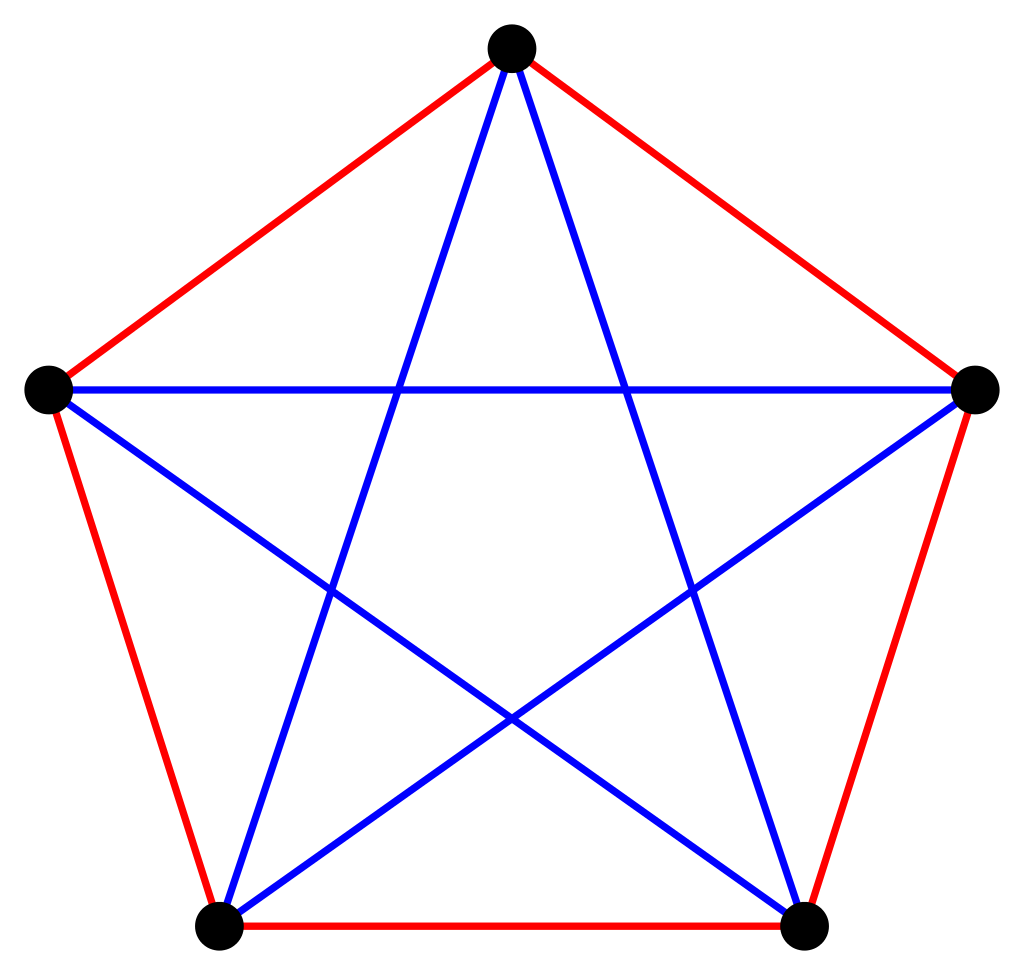
\includegraphics[scale=0.1]{1-1.png}
    \end{center}
    To prove $R(3,3)\leq 6$, we consider a vertex $v$. By pigeonhole principle, there is some color (For simplicity, blue) appears at least 3 times between $v$ and its neighbors. Then edges between these neighbors must be red, but this will induced a red triangle.
\end{proof}

\begin{example}
    $R(k,k)>(k-1)^{2}$.
\end{example}

\begin{proof}
    Take $(k-1)$ many $K_{k-1}$ and color edges in each $K_{k-1}$ red and edges between different $K_{k-1}$ blue. Then we have $(k-1)^{2}$ vertices with no monochromatic $K_{k}$.
\end{proof}

In 1947, \Erdos{} \cite{Erds1947SomeRO} improved the lower bound from polynomial to exponential using probability methods:

\begin{theorem}[\Erdos{}, 1947 \cite{Erds1947SomeRO}]
    $R(k,k)>n=(1+o(1))\frac{k}{\sqrt{2}e}2^{k/2}$.
\end{theorem}

\begin{proof}
    Consider a random edge-coloring of $K_{n}$, we color each edge with a $1/2$ chance of either red or blue. Then the expectation number of monochromatic $K_{k}$ is $$\mathbb{E}[\text{\# monochromatic } K_{k}]=\binom{n}{k}\cdot\mathbb{P}(\text{a fixed k-set is monochromatic})=\binom{n}{k}\cdot\left(\frac{1}{2}\right)^{\binom{k}{2}}\cdot 2<1.$$
    So there exists a two-edge-coloring on $K_{n}$ with no monochromatic $K_{k}$.
\end{proof}




\newpage

\section{Lecture 2}

\subsection{\Erdos{}-Szekeres Problem}

Another famous Ramsey-type result is the \Erdos{}-Szekeres problem.

\begin{problem}
     Consider a sequence of natural numbers, for examples, $10,5,7,4,6,\cdots$, now we wonder that how long a monotone subsequence (either increasing or decreasing) can be.
\end{problem}

\Erdos{}-Szekeres problem gives us a bound on length of sequence to guarantee appearance of a given length monotone subsequence. It is a Ramsey-type problem in extremal combinations, and it introduces the structure in the distinct natural number sequence. 

\begin{theorem}[\Erdos{},Szekeres \cite{Erdos-SzekeresThm}]
   For any sequence of distinct natural numbers of size $(k-1)^2+1$, there is a monotone sequence of size $k$.
\end{theorem}

IDEA: Pigeonhole/averaging argument

\begin{proof}
  Consider an arbitary sequence $a_1,a_2,\ldots,a_{(k-1)^2+1}$, $a_i\in \mathbb{N}$.
  Label each number of $a_i$ by the length of longest monotone increasing sequence ending at $a_i$: $\ell(a_i)$. $\ell(a_i)\le k-1$, otherwise, we have found the $k$-length monotone increasing sequence.
  
  By pigeonhole principle, there is at least one label $r\in[k-1]$, such that $$\left | \left \{i: \ell (a_i)=r \right \}  \right | \ge \left \lfloor \frac{(k-1)^2+1}{k-1}  \right \rfloor +1=k$$
  i.e. there exist $a_{i_1},a_{i_2},\ldots,a_{i_k}$
        such that $$\ell (a_{i_j})=r,\forall j\in [k] $$
  
  $a_{i_1},a_{i_2},\cdots,a_{i_k}$ form a k-length monotone decreasing subsequence. Otherwise, without loss of generality, we assume $a_{i_1}<a_{i_2}$. Then we can make up a $(r+1)$-length monotone increasing subsequence by adding $a_{i_2}$ to the monotone increasing subsequence ending at $a_{i_1}$. That means $\ell (a_{i_2}) \ge r+1$, thus lead to contradiction.
\end{proof}

\begin{remark}
    The bound is optimal. Tight example: $$(k-1,k-2,\ldots,1), (2k-2, 2k-3,\ldots,k),\ldots,((k-1)^2,(k-1)^2-1,\ldots,(k-1)(k-2)+1)$$
    This is a sequence of size $(k-1)^2$ without a monotone  subsequence of size $k$.
\end{remark}

\begin{remark}
    This theorem can be expand to an asymmetric version.
    For any sequence of distinct natural numbers of size $(a-1)(b-1)+1$, there is a monotone increasing sequence of size $a$ or a monotone decreasing sequence of size $b$.
\end{remark}

\begin{definition}[Tournament]
  A \emph{tournament} is an orientation of complete graph.
\end{definition}

\begin{exercise}
    For any tournament of order $n$, there is a directed Hamiltonian path (a path that visited all vertices).
\end{exercise}

\subsection{Sperner's Theorem}

Let us consider the $2^{[n]}$(the power set of $[n]$), there are two ways to visualize it.

Firstly, we visualize it by visualize $\{0,1\}^n$.

\begin{definition}[Hypercube]
     A \emph{hypercube} is a graph $G=(V,E)$, where $V:=\{0,1\}^n$ and $E:=\{xy:x \text{ and } y \text{ differ at 1 place} \}$.
\end{definition}

\begin{example}
    When $n=3$, a hypercube as illustrated below
    \begin{center}
            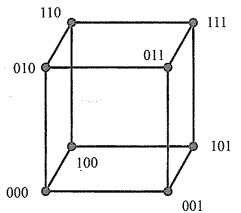
\includegraphics[scale=0.9]{2-1.jpg}
    \end{center}
\end{example}

The second way is to consider the family of all subsets of $[n]$. Let $H=(V,E)$ be a graph with $V:=\left \{ A : A\subseteq[n] \right \} $ and $E:=\left \{ xy : \left | \left | x \right | -\left | y \right |  \right |=1 \text{ and }
x\subseteq y \text{ or } y \subseteq x\right \} $.

\begin{example}
    When $n=3$, $H$ as illustrated below.
    \begin{center}
            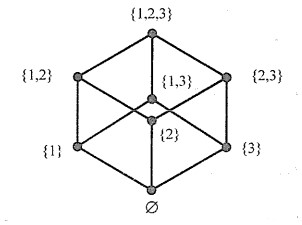
\includegraphics[scale=0.9]{2-2.jpg}
    \end{center}
\end{example}

There is a natural corresponding between the two visualize ways.
The map $\phi:\{0,1\}^n \to \left \{ A : A\subseteq[n] \right \},\alpha=(a_1 a_2 \cdots a_n) \to 
    \left \{ x : a_x=1 \right \}$ is a isomorphism of the two graphs.

The Sperner's Theorem is about finding the largest family of sets that satisfied no set is contained by another set. 

\begin{definition}[Antichain]
  A family of sets $\mathcal{A}\subseteq 2^{[n]}$ is an \emph{antichain} if no element of $\mathcal{A}$ is a subset of another.
\end{definition}

We can see that if one set is contained by another set, then the two sets must have different size. So we have a natural example.

\begin{example}
    Any level (all sets of the same size) is an antichain.
\end{example}

\begin{observation}
    $$ \# \text{ all size-k set}=  \binom{n}{k} 
   \le \binom{n}{\lfloor n/2\rfloor}$$
\end{observation}

\begin{theorem}[Sperner\cite{SpernerThm}]\label{SpernerThm}
    The size of the largest antichain in $2^{[n]}$ is $\binom{n}{\lfloor n/2\rfloor}$.
\end{theorem}

We would use the Lubell-Yamamoto-Meshalkin inequality (L-Y-M inequality) to prove the theorem.

\begin{theorem}[L-Y-M inequality \cite{LYMinequality}]\label{thm:LYM}
    For any antichain $\mathcal{F}\subseteq 2^{[n]}$, we have 
\begin{align*}
    \sum_{F\in \mathcal{F}}\frac{1}{\binom{n}{|F|}}\le 1
\end{align*}
\end{theorem}

\begin{proof}[Proof 1: double counting]
    We count the number of all permutation of $[n]$.
    
    It is well known that $\#\text{ all permutation of [n]} = n !$. 
    
    On the other hand, for $F \in \mathcal{F}$, let $P(F)$ be 
    the set of the permutation satisfying that all element in 
    $F$ appears before the element not in $F$. It can be seen 
    that 
    $ \left | P(F) \right | = \left | F \right | ! ( n - \left | F \right |) ! $.
    
    Noticed that for two different set $F,F' \in \mathcal{F}$,
    $$P(F) \cap P(F') = \emptyset $$
    otherwise there exists a permutation  
    $(a_1a_2\cdots a_n)$ such that $F=\left \{ a_i:i\le j \right \} $ and $F'=\left \{ a_i:i\le k \right \} $,
    we have $F \subseteq F'$ or $F' \subseteq F$, which make a contradiction.
    
    Thus we have $$\sum_{F \in \mathcal{F}}\left | P(F) \right | = \sum_{F \in \mathcal{F}}\left | F \right | !(n-\left | F \right | )!\le n!$$
    
    Divided by $n!$ on both side, then we have 
    \begin{align*}
        \sum_{F\in \mathcal{F}}\frac{1}{\binom{n}{|F|}}\le 1
    \end{align*}
\end{proof}

Noticed that the statement "There is ten elements in a set" is equivalent to "The probability of picking a certain element is $10\%$ ". 
The fact suggests that when we use the double-counting method on a set in a proof, we can also use the probabilistic method to rewrite the proof.

\begin{proof}[Proof 2: probabilistic method]
  One can find more details of the proof in \textit{The Probabilistic Method, 4th Edition}\cite{TheProbabilisticMethod}
  
  Take a uniform random permutation $\sigma=\left \{ \sigma_1,\sigma_2,\cdot,\sigma_n \right \}$ from $[n]$, denoted it by $\sigma \sim S_n $. 
  $\forall k \in [n]$, let $I_k=\left \{ \sigma_1,\sigma_2,\cdot,\sigma_k \right \} $, obviously 
  $I_1 \subset I_2 \subset \cdots \subset I_n $, thus there is at most one of them can be in $\mathcal{F}$.
  Note that $I_k \sim \binom{[n]}{k}$, so we can calculate the number of $I_k$ in $\mathcal{F}$.
  $$1 =\text{max} \#I_k \text{ in } \mathcal{F} \ge \sum_{k=1}^{n}Pr(I_k \in \mathcal{F}) = \sum_{k=1}^{n}\frac{f_k}{\binom{n}{k}}
  = \sum_{F\in \mathcal{F}}\frac{1}{\binom{n}{\left | F \right |    }}$$ in here, $f_k$ means the number of k-sets in $\mathcal{F}$.
\end{proof}

\begin{proof}[Proof of \ref{SpernerThm}
:using L-Y-M inequality]
    For any antichain $\mathcal{F}\subseteq 2^{[n]}$,
    $\left | \mathcal{F} \right | \le \binom{n}{\lfloor n/2\rfloor}$, for
    $$1 \ge \sum_{F \in \mathcal{F}}\frac{1}{\binom{n}{\lfloor \left | F \right | \rfloor}} \ge \sum_{F \in \mathcal{F}}\frac{1}{\binom{n}{\lfloor n/2\rfloor}}
    = \left | \mathcal{F} \right |\frac{1}{\binom{n}{\lfloor n/2\rfloor}} $$

    On the other hand, all sets of size $\lfloor n/2\rfloor$ is a antichain of size $\binom{n}{\lfloor n/2\rfloor}$ .
\end{proof}

\subsection{Topic 1:Extremal Graph Theory}

One of the most classical problems in extremal graph theory, nowadays so-called \Turan{}-type problem, is:

\begin{problem}[\Turan{} problem]\label{TuranProblem}
    Max number of edges in an $n$-vertex $H$-free graph $G$?
\end{problem}

\begin{definition} [\Turan{}/extremal number of $H$] 
    The \emph{\Turan{}/extremal number of $H$} is defined as $\ex(n,H)$
    \begin{align*}
        \ex(n,H)=\max\{e(G): G \text{ is an $n$-vertex, $H$-free graph}\}
    \end{align*}
\end{definition}

\begin{example}
    Mantel's theorem means $ex(n,K_3)=\left \lfloor 
    \frac{n^2}{4} \right \rfloor$.
\end{example}

\Turan{} solved \ref{TuranProblem} as $H$ is a clique, and he pointed out that the so-called \Turan{} graph is the unique extremal graph.

\begin{definition}[\Turan{} graph]
   \emph{\Turan{} graph} $T_{n,r}$ is the $n$-vetex complete $r$-partite graph with each partition set of size $\lfloor n/r \rfloor$ or $\lceil n/r\rceil$. 
\end{definition}

\begin{example}
    $T_{7,2}=K_{2,2,3}$ as illustrated below.
    \begin{center}
        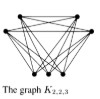
\includegraphics[scale=1.5]{2-4.jpg}
    \end{center}
\end{example}

There are many useful properties of \Turan{} graph, we state two of them and leave the proofs of them as exercise.

\begin{exercise}
    $$ e(T_{n,r}) = (1-\frac{1}{r})\frac{n^2}{2}-O(r)
    \le (1-\frac{1}{r})\frac{n^2}{2}$$
    with equality if and only if $n$ is divisible by $r$.
\end{exercise}

\begin{exercise}\label{most number among CMG}
    Among all complete $r$-partite graphs on $n$ vertices, $T_{n,r}$ has the most number of edges.
\end{exercise}

\begin{theorem}[\Turan{}, 1941\cite{Turan1941Thm}]
    \label{TuranThm}
   $$\ex(n,K_{r+1})=e(T_{n,r})$$ 
    Furthermore, $T_{n,r}$ is the unique extremal graph.
\end{theorem}

As Mentel's theorem is a special case of \Turan{}'s theorem when $r=2$, the two proofs of Mentel's theorem can be extend to proof \Turan{}'s theorem. We leave it as exercise.

\begin{exercise}
   Extend the two proofs of Mentel's theorem to prove \Turan{}'s theorem.
\end{exercise}

By \ref{most number among CMG}, we can see that if the statement \emph{for all $n$-vertex $H$-free graph $G$, there exists a r-partite graph $F$ such that $e(G)\le e(F)$} is true, then we have completed the proof. To prove the statement, we use the method so-called \emph{Zykov's symmetrization}.

\begin{proof}[Proof 3: Zykov's symmetrization]
    For graph $G=(V,E)$, Sort the points in degrees from largest to smallest: $v_1,\ldots,v_n$.
    for $v_i$, find the smallest $j<i$, such that $v_iv_j \notin E$, do symmetrization(i.e. replace $v_i$ by a copy of $v_j$) , the number of edges would not decrease and the new graph remains an n-vertex $K_{r+1}$-free graph(since a clique cannot contain both a vertex and its copy). 
\begin{center}
    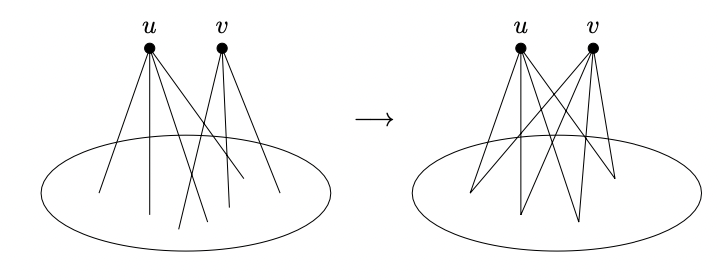
\includegraphics[scale=0.9]{2-3.png}
\end{center}
    The process ends in n-steps. At the end, the non-adjacent is an equivalence relation. Thus we obtain a complete multipartite graph, whose number of parts $k<n$. As \ref{most number among CMG} shown, we obtain the conclusion.
\end{proof}

\newpage

\section{Lecture 3}

\subsection{Motzkin-Straus Symmetrization}
Motzkin-Straus symmetrization can be viewed as a continuous version of Zykov's symmetrization. Before rigorously defining Motzkin-Straus symmetrization, recall some basic linear algebra.

\begin{definition}[adjacency matrix]
    Let $G$ be an $n$-vertex graph and $v_1,...,v_n$ be an ordering of its vertices. The \emph{adjacency matrix} of $G$ is the $n \times n$ symmetric $0/1$-matrix $A_G = (a_{ij})_{i,j\in [n]}$ in which $a_{ij} = 1$ if and only if $v_i v_j \in E(G)$.
\end{definition}

Given an $n$-vertex graph $G$ and $\boldsymbol{x} \in \mathbb{R}^n$, the following quadratic form is called \emph{Lagrangian function} of graph $G$
\[
\lambda_G(\boldsymbol{x}) = \frac{1}{2} \boldsymbol{x}^T A_G \boldsymbol{x} = \frac{1}{2} \sum_{i,j \in [n]} x_i x_j a_{ij} = \sum_{v_i v_j \in E(G)} x_i x_j.
\]

Write $\Delta^{n-1}$ for the $(n-1)$-dimensional simplex
\[
\Delta^{n-1} = \{\boldsymbol{x} \in \mathbb{R}^n: \forall i\in [n], x_i \geq 0, \text{ and } \sum_{i=1}^n x_i = 1\}.
\]

The \emph{Lagrangian} of $G$ is
\[
\lambda(G) = \sup_{x \in \Delta^{n-1}} \lambda_G (\boldsymbol{x}).
\]

Basically, the Lagrangian function of $G$ is the number of edges in a weighted blow-up of $G$. Every vector $\boldsymbol{x}$ in the $(n-1)$-dimensional simplex $\Delta^{n-1}$ corresponds to a weighted blow-up $G_{\boldsymbol{x}}$ of $G$. Then, $\lambda_{G}(\boldsymbol{x}) = e(G_{\boldsymbol{x}})$.  

\begin{theorem}[Motzkin-Straus \cite{Motzkin1965sym}, 1965]\label{MSsymmetrization}
    For any $K_{r+1}$-free $n$-vertex graph $G$ and $\boldsymbol{x} \in \Delta^{n-1}$, there exists $\boldsymbol{y} \in \Delta^{n-1}$ such that $\lambda_G(\boldsymbol{y}) \geq \lambda_G(\boldsymbol{x})$ and $\supp(\boldsymbol{y})$ induces a clique in $G$, where $\supp(\boldsymbol{y})$ is the support of $\boldsymbol{y}$ which is the set of non-zero coordinates of $\boldsymbol{y}$. In particular, 
    \[
    \lambda(G) = \frac{1}{2} (1-\frac{1}{r}).
    \]
\end{theorem}

Let $\boldsymbol{x} = (1/n, 1/n, ..., 1/n)^T \in \Delta^{n-1}$. Then $\lambda_G = e(G)/n^2 \leq \lambda(G) = \frac{1}{2} (1-\frac{1}{r})$. Thus, we recover a weaker version of \Turan{}'s Theorem.

The idea to prove this theorem is 'mass transportation': if $\boldsymbol{x}$ has mass on two coordinates that correspond to two non-adjacent vertices, then we move weight from one coordinate to another one without decreasing $\lambda_G(\cdot)$.

\begin{proof}[Proof of Theorem \ref{MSsymmetrization}]
    Take $\boldsymbol{y} \in \Delta^{n-1}$ with minimal support such that $\lambda_G(\boldsymbol{y}) \geq \lambda_G(\boldsymbol{x})$. We shall prove that $\supp(\boldsymbol{y})$ induces a clique. 

    Suppose there are two non-adjacent vertices corresponding to the coordinates in $\supp(\boldsymbol{y})$, say $\{1,2\}$. Let $\boldsymbol{z} = (z, -z, 0, ..., 0)^T$. Note that $\boldsymbol{y} + \boldsymbol{z} \in \Delta^{n-1}$ and $\boldsymbol{z}^T A_G \boldsymbol{z} = 0$, since $\{1, 2\} \not\in E(G)$. Then
    \[
    \lambda_G(\boldsymbol{y} + \boldsymbol{z}) = \frac{1}{2}(\boldsymbol{y} + \boldsymbol{z})^T A_G (\boldsymbol{y} + \boldsymbol{z}) 
    = \frac{1}{2} \boldsymbol{y}^T A_G \boldsymbol{y} + \boldsymbol{z}^T A_G \boldsymbol{y} + \frac{1}{2} \boldsymbol{z}^T A_G \boldsymbol{z} = \frac{1}{2} \boldsymbol{y}^T A_G \boldsymbol{y} + \boldsymbol{z}^T A_G \boldsymbol{y}.
    \]
    Then $\lambda_G(\boldsymbol{y} + \boldsymbol{z})$ is linear in $\boldsymbol{z}$. Thus, we can choose $\boldsymbol{z}$ such that $\lambda_G(\boldsymbol{y} + \boldsymbol{z}) \geq \lambda_G(\boldsymbol{y}) \geq \lambda_G(\boldsymbol{x})$ and $\supp(\boldsymbol{y} + \boldsymbol{z}) \subsetneq \supp(\boldsymbol{y})$. This contradicts the minimality of $\supp(\boldsymbol{y})$. 
\end{proof}

\begin{exercise}[Local version of \Turan{}'s Theorem; Bradac \cite{bradavc2022generalization}, Malec-Tompkins \cite{Malec2023local}]
    For every $n$-vertex graph $G$, we have
    \[
    \sum_{e \in E(G)} \frac{k(e)}{k(e)-1} \leq \frac{n^2}{2},
    \]
    where $k(e)$ is the size of largest clique in $G$ containing the edge $e$.
\end{exercise}

The 'in particular' part of Theorem \ref{MSsymmetrization} amounts to proving the following. 

\begin{exercise}
    $\lambda(K_r) = \frac{1}{2} (1 - \frac{1}{r})$.
\end{exercise}

\subsection{Caro-Wei Theorem}

\begin{definition}[independent set]
    Let $G$ be a graph. We say $S \subseteq V(G)$ is an \emph{independent set} if $S$ induces no edge. The \emph{independence number} of $G$, denoted by $\alpha(G)$, is the size of largest independent set in $G$. 
\end{definition}

\begin{theorem}[Caro \cite{caro1979new}, Wei \cite{wei1981lower}]
    For any graph $G$, we have
    \[
    \alpha(G) \geq \sum_{v \in V(G)} \frac{1}{d(v) + 1}.
    \]
\end{theorem}

The lower bound means that we need to find an independent set of large size. We will construct such an independent set probabilistically by the First Moment Method. 

\begin{proof}
    Consider a uniformly random permutation $\sigma$ of $V(G)$. Define 
    \[
    I := \{v \in V(G): v \text{ precedes all vertices in $N(v)$}\}.
    \]
    Observe $I$ is an independent set. It suffices to show that $\mathbb{E}|I| = \sum_{v \in V(G)} 1/(d(v)+1)$ as then there exists $I$ such that $\alpha(G) \geq |I| \geq \mathbb{E}|I|$. Since $\sigma$ is a uniformly random permutation, $\Pr(v \in V(G)) = 1/(d(v) + 1)$.
    \[
    \mathbb{E}|I| = \sum_{v \in V(G)} \Pr(v \in I) = \sum_{v \in V(G)} \frac{1}{d(v) + 1}.
    \]
\end{proof}


\subsection{\Erdos{}-Stone-Simonovits Theorem}
\Erdos{}-Stone-Simonovits Theorem is considered as one of the fundamental theorems in extremal graph theory. The \Turan{}'s Theorem determines the extremal number of cliques. The next natural question is what if we forbid a generic graph $H$. The \Erdos{}-Stone-Simonovits Theorem gives a satisfactory answer by telling us the extremal number of $H$ is determined by another essential parameter in graph theory.

\begin{definition}[chromatic number]
    Given a graph $H$, its \emph{chromatic number}, denoted by $\chi(H)$, is the minimal number $k$ such that we color vertices of $H$ by $k$ colors so that no adjacent vertices receive the same color.
\end{definition}

\begin{theorem}[\Erdos{}-Stone-Simonovits Theorem \cite{erdos1966limit, erdos1946linear}, 1946]{}{} \label{ESS}
    For any graph $H$, 
    \[
    \ex(n,H) = \left(1- \frac{1}{\chi(H) - 1} \pm o(1) \right) \frac{n^2}{2}.
    \]
    Rigorously, for any $\varepsilon > 0$ and graph $H$, there exists $n_0 = n_0(\varepsilon,H)$ such that, for any $n \geq n_0$,
    \[
    \ex(n,H) = \Big(1-\frac{1}{\chi(H)-1} \pm \varepsilon \Big)\frac{n^2}{2}.
    \]
    Here $x = a \pm b$ means $a-b \leq x \leq a+b$.
\end{theorem}


\begin{remark}
    The \Erdos{}-Stone-Simonovits Theorem determines asymptotically $\ex(n,H)$ for all non-bipartite graph $H$. While for bipartite graph $H$, we only get $o(n^2)$ as  an upper bound for $\ex(n, H)$.
\end{remark}


\textbf{Lower bound of the \Erdos{}-Stone-Simonovits Theorem:} Let $\chi(H) = r+1$. We can find an $n$-vertex $H$-free graph with at least $(1 - \frac{1}{r} - \varepsilon)\frac{n^2}{2}$ edges. \Turan{} graph $T_{n,r}$ has about $(1 - \frac{1}{r})\frac{n^2}{2}$ edges and contains no copy of $H$ in $T_{n,r}$ as $\chi(H) > \chi(T_{n,r})$.


\textbf{Upper bound of the \Erdos{}-Stone-Simonovits Theorem:} For the upper bound, we need to show the following. For any $n$-vertex graph $G$ with at least $(1 - \frac{1}{r} + 2\varepsilon)\frac{n^2}{2}$ edges, we can always find a copy of $H$ in $G$. Let $t$ be the number of vertices of $H$. We are actually gonna prove a slightly stronger result $H \subseteq K_{t,..., t} \subseteq G$, where $K_{t,...,t}$ is a $(r+1)$-partite complete graph. We will do so by induction on $r$. 

\begin{lemma}\label{subgraphlem}
    For any $0 < \varepsilon < c <1$, there exists $n_0 = n_0(\varepsilon,c)$ such that for any $n \geq n_0$, the following holds. For any $n$-vertex $G$ with at least $cn^2/2$ edges, there exists a subgraph $G' \subseteq G$ on $n' \geq \sqrt{\varepsilon}n/2$ vertices such that $\delta(G') \geq (c-\varepsilon)n'$.
\end{lemma}

The idea to prove this lemma is to keep removing vertices with low degree from $G$.

\begin{exercise}
    Prove Lemma \ref{subgraphlem}.
\end{exercise}

\begin{proof}[Proof of the \Erdos{}-Stone-Simonovits Theorem]
    By Lemma \ref{subgraphlem}, there is a $G' \subseteq G$ on $n' \geq \sqrt{\varepsilon}n/2$. Rewrite $G$ for $G'$. Start with $n$-vertex $G$ with $\delta(G) \geq (1-\frac{1}{r}+\varepsilon)n$. Our goal is to embed $K_{t,...,t} \subseteq G$. We will do induction on the number of parts, say $s(1\leq s \leq r+1)$, in $K_{t,...,t}$, that for any $t$, there exist $n_0 = n_0(t,s)$ such that for any $n \geq n_0$ and $n$-vertex graph $G$ with $\delta(G) \geq ((1-\frac{1}{r}+\varepsilon)n)$ we have $G$ contains a copy of $s$-partite complete graph $K_{t,...,t}$. 

    When $s = 1$, the result is trivially true. Suppose the result is true for all $s \leq r$. Now we need to embed $(s+1)$-partite complete graph $K_{t,...t}$ into $G$. 

    By induction hypothesis, there exists an $s$-partite complete graph $K_{T,...,T} \subseteq G$, where $T = \frac{4}{r\varepsilon}t$, on partite sets, say $X_1,...,X_s$. Let $Y = V(G) \setminus (\cup_{i=1}^s X_i)$.

    \begin{claim}
        Let $Z \subseteq Y$ be the set of all vertices with at least $\frac{r\varepsilon}{4}|X_i| = t$ neighbors in each $X_i, i\in[s]$. Then $|Z| \geq \frac{r\varepsilon}{4}n$.
    \end{claim}

    \begin{proof}
        We denote the structure $(y,x_1,x_2,\cdots,x_s)$, where $y\in Y,x_i\in X_i,x_iy\in E(G),i\in [s]$ as a \emph{star}, and we will do double counting on the number of stars, says $N$, to finish the proof. 

        \begin{itemize}
            \item \textbf{Lower bound of $N$:}
            
            Fix an $s$-tuple $(x_1,\cdots,x_s)\in X_1\times X_2\times\cdots\times X_s$, then for sufficiently large $n$, we have
            \begin{align*}
                &\#\{\text{Common neighbors of $x_i$}\}\\
                \geq&\sum_{i=1}^{s}d(x_{i})-(s-1)n-sT\\
                \geq&(1-\frac{1}{r}+\varepsilon)ns-(s-1)n-s\frac{4}{r\varepsilon} t\\
                =&n-(n(\frac{1}{r}-\varepsilon)+\frac{4}{r\varepsilon}t)s\\
                \geq&nr\varepsilon-\frac{4}{\varepsilon} t\\
                \geq&\frac{nr\varepsilon}{2},
            \end{align*}
            where the first inequality is obtained by considering the limiting case that all vertices in $Y$ is common neighbors of $s$ or $s-1$ vertices in $\{x_1,\cdots,x_s\}$. By counting all possible values of $s$-tuple, we obtain a lower bound of $N$:
            \begin{equation}\label{eq:Lbd of N in E-S thm}
                N\geq\prod_{i=1}^{s}|X_{i}|\cdot\#\{\text{Common neighbors of $x_i$}\}\geq\prod_{i=1}^{s}|X_{i}|\cdot \frac{nr\varepsilon}{2}.
            \end{equation}

            \item \textbf{Upper bound of $N$:}

            Let $Z'\subseteq Y$ denote the set of vertices involved in more than $\frac{r\varepsilon}{4}\prod_{i=1}^{s}|X_{i}|$ stars, it is easy to check $Z'\subseteq Z$, then we can obtain an upper bound of $N$ as follows by dividing $Y$ into $Z'$ and the other:
            \begin{equation}\label{eq:Ubd of N in E-S thm}
                N\leq |Z'|\cdot\prod_{i=1}^{s}|X_i|+n\cdot\frac{r\varepsilon}{4}\prod_{i=1}^{s}|X_i|.
            \end{equation}
        \end{itemize}
        Combining the inequality \eqref{eq:Lbd of N in E-S thm} and the inequality \eqref{eq:Ubd of N in E-S thm}, we can get the conclusion
        \[
        |Z|\geq|Z'|\geq\frac{r\varepsilon}{4}n.
        \]
    \end{proof}
    
    Each vertex in $Z$ gives rise to a copy of $(s+1)$-partite complete graph $K_{1,t,...,t}$ with the size-$t$ part in each $X_i$. The number of choices for $t$-sets $X'_i \subseteq X_i = \binom{T}{t}^s$. By the Pigeon Hole Principle, there are at least
    \[
    \frac{|Z|}{\binom{T}{t}^s} \geq \frac{r\varepsilon}{4 \binom{T}{t}^s} \cdot n \geq t
    \]
    vertices in $Z$ sharing the same $t$-sets in $X_1,...,X_s$ as neighbors. The last inequality holds when $n$ is sufficiently large. Thus, we find a $(s+1)$-partite complete graph $K_{t,...,t} \subseteq G$. 
\end{proof}

\begin{remark}
    If we do the calculation carefully, the proof actually gives that for an $n$-vertex $(1-\frac{1}{r}+\varepsilon)\frac{n^2}{2}$-edge graph $G$, we can embed a $\Omega(\log n)$-blow-up of $K_{r+1}$ into $G$.
\end{remark}


\newpage


\section{Lecture 4}

To review the \Erdos{}-Stone-Simonovits Theorem, let's succinctly summarize the entire proof by breaking it down into several key steps. Each of these steps employs a highly effective technique that recurs in numerous other mathematical problems.

\begin{itemize}

    \item \textbf{Step 1: Bootstrapping average degree to minimum degree.}
    
    Bootstrapping refers to the process of starting with some initial conditions or assumptions and gradually strengthening them to derive a more powerful property. In the context of this theorem, we begin with an average degree condition and improve it to a minimum degree condition by sacrificing a small constant factor ($\varepsilon$). This creates a subgraph with a high minimum degree, allowing us to work with a graph that satisfies stronger conditions.
    
    \item \textbf{Step 2: Induction on the number of parts to build $K_{t, \ldots, t}$.}
    
    \item \textbf{Step 3: Claim that many vertices ($Z$) have high degree to each $X_i$.}
    
    By double-counting the number of stars.
    
    \item \textbf{Step 4: Using the pigeonhole principle to obtain $X_{s+1}$.}
    
\end{itemize}

\subsection{Applications of \Turan{}'s Theorem}

The first application we will introduce is a geometric theorem:

\begin{theorem}[\Erdos{}]
    For any arrangement $P$ of $n$ points in $\R^{2}$ with diameter \footnote{The \emph{diameter} is the maximum distance between any two distinct points $x, y$ in the set.} $1$, the number of pairs of points in $P$ with distance strictly greater than $\frac{1}{\sqrt{2}}$ is at most $\frac{n^2}{3}$.
\end{theorem}

\begin{proof}
    Let us denote the distance between two points $x$ and $y$ as $\text{dist}(x, y)$. We define an auxiliary graph $G$ on $n$ vertices, where the vertex set $V(G) = P$, and two vertices $x$ and $y$ are adjacent in $G$ (i.e., $xy \in E(G)$) if and only if $\text{dist}(x, y) > \frac{1}{\sqrt{2}}$. If we can prove that $G$ is $K_4$-free, then by \Turan{}'s Theorem, we have $e(G) \leq (1 - \frac{1}{3}) \frac{n^2}{2} \leq \frac{n^2}{3}$, which would prove the desired statement.
    
    Suppose, for the sake of contradiction, that there exists a copy of $K_4$ as a subgraph of $G$. This implies that there are four points in the plane such that the distance between every pair of them is greater than $\frac{1}{\sqrt{2}}$.

    \begin{figure}[H]
        \centering
        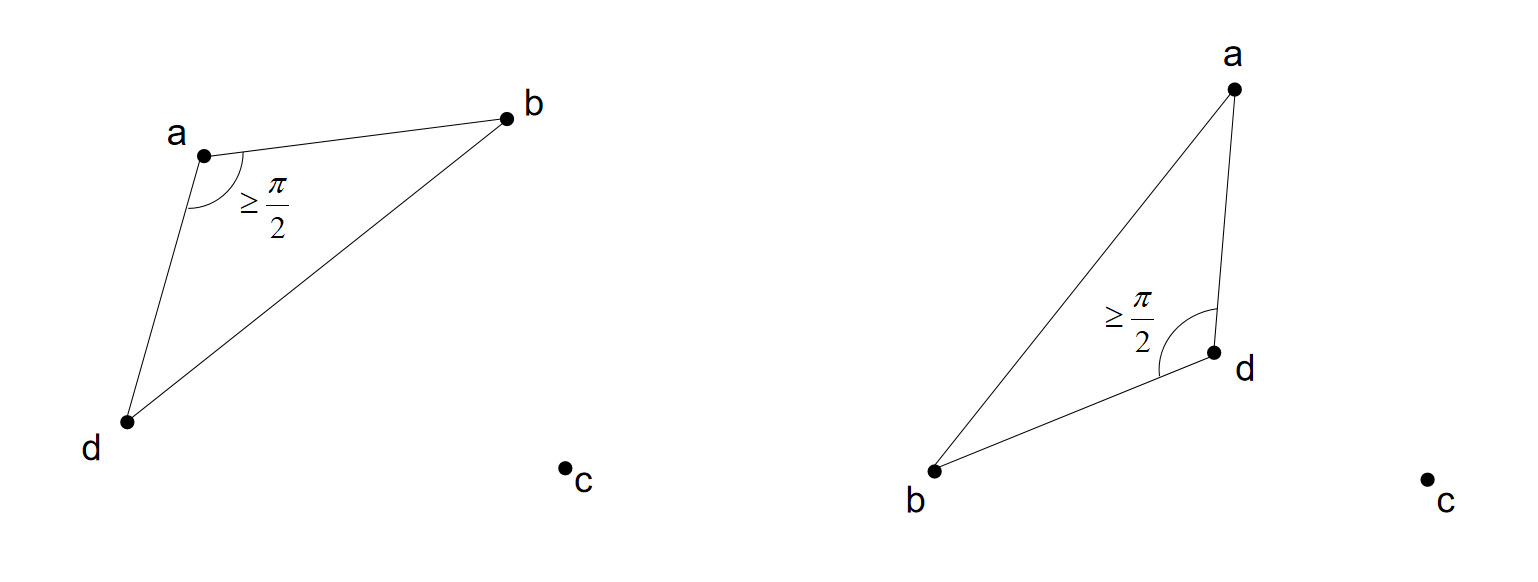
\includegraphics[scale=0.3]{4-1.png}
        \caption{Two kinds of arrangements of 4 points in the plane.}
        \label{fig:4-1}
    \end{figure}

    We notice that among these four points, there must exist three points such that the angle formed by them is not acute (we can verify this by classifying the arrangements based on whether they form convex quadrilaterals, as shown in Figure \ref{fig:4-1}\footnotemark). This implies that the diameter of the four points is strictly greater than $1$, which contradicts the given condition.

    Therefore, we have proved that $G$ is $K_4$-free, and by \Turan{}'s Theorem, the number of edges in $G$ is at most $\frac{n^2}{3}$, which completes the proof.
\end{proof}

\subsection{Second proof of the \Erdos{}-Stone-Simonovits Theorem}

The first proof of the \Erdos{}-Stone-Simonovits Theorem is a classical one, and now we would like to present a conceptually simpler and more modern proof.

\begin{definition}[Homomorphism]
    A \emph{homomorphism} from graph $H$ to graph $G$ is a map $\varphi: V(H) \rightarrow V(G)$ preserving the adjacencies, i.e., $\forall uv \in E(H) \Rightarrow \varphi(u)\varphi(v) \in E(G).$ (We will abbreviate it as $\varphi: H \rightarrow G$ later on.)
\end{definition}

We should note that this is different from subgraph containment, since it's not necessary for a graph homomorphism to be injective, see Figure \ref{fig:4-2}.

\begin{figure}[H]
    \centering
    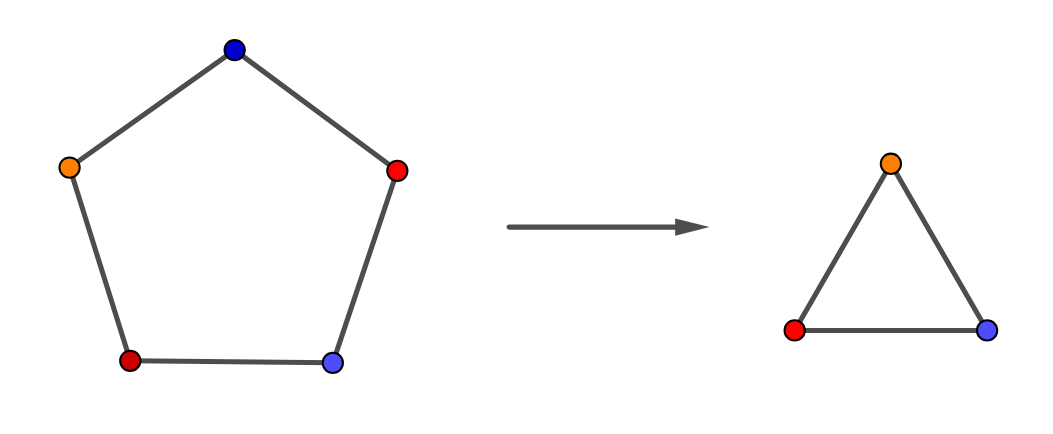
\includegraphics[scale=0.7]{4-2.png}
    \caption{A homomorphism from $C_{5}$ to $K_3$.}
    \label{fig:4-2}
\end{figure}

\begin{exercise}
    There exists a homomorphism $\varphi: H \rightarrow K_r$ if and only if $\chi(H) \leq r$.
\end{exercise}

\begin{exercise}
    We denote a $n$-circle as $C_n$, prove that:
    
    \begin{enumerate}
        \item There exists a homomorphism from $C_7$ to $C_5$.

        \item There is no homomorphism from $C_5$ to $C_7$.
    \end{enumerate}
\end{exercise}

If there exists a homomorphism $\varphi: H \rightarrow G$, we say that $G$ is a \emph{homomorphic image} of $H$.

\begin{exercise}
    Prove that $K_{\chi(H)}$ is a homomorphic image of $H$.
\end{exercise}

\begin{definition}[Edge density]
    For a graph $G$ with $n$ vertices, we define its \emph{edge density} as $\tau = e(G) / \binom{n}{2}$.
\end{definition}

\begin{lemma}[Embedding Lemma]
    Let $H$ be a graph, then the following holds for all sufficiently large $n$:

    For all $n$-vertices $H$-free graph $G$ with edge $\tau> 0,$ there exists a (reduced) graph $R$ with edge density $\geq \tau-o(1),$ and $R$ contains no homomorphism image of $H$(We also call the second property as $H$-hom-free.).
\end{lemma}

This Lemma is very useful, for it is a Bootstrap, we can Bootstrap an $H$-free condition to $H$-hom-free condition without lossing much on edge density. We may remain the proof of Embedding Lemma behind, now we can give another proof of \Erdos{}-Stone-Simonovits Theorem.


\begin{proof}[Proof 2 of the \Erdos{}-Stone-Simonovits Theorem]
    Here we only give the proof of Upper bound. By Embedding Lemma, there exists a subgraph $R$ of $G$ with edge density $\geq \tau-o(1),$ and $R$ contains no homomorphism image of $H$, $\chi(H)=r+1$, so $R$ is $K_{r+1}$-free. 

    Applying \Turan{}'s Theorem on $R$, we get
    \[\tau-o(1)\leq\text{edge density of $R$}\leq 1-\frac{1}{r}+o(1). \]
    which means $\tau\leq 1-\frac{1}{r}+o(1).$ By the definition of the edge density, we are done.
\end{proof}

\begin{remark}
    The embedding Lemma reduces the \Erdos{}-Stone-Simonovits Theorem to \Turan{}'s Theorem.
\end{remark}

\subsection{Supersaturation}

Now we have proved the \Erdos{}-Stone-Simonovits Theorem that $\ex(n,H) = \left(1- \frac{1}{\chi(H) - 1} \pm o(1) \right) \frac{n^2}{2},$ then there is a natural question: What happens when we have more edges than this threshold? By \Erdos{}-Stone-Simonovits Theorem, we know that there are at least one copy of (the forbidden graph) $H$. In fact, we shall see that ``many" copies emerge, such phenomenon is called ``\emph{Supersaturation}". Some examples are as follows.

\begin{theorem}[Rademacher\cite{erdos1962Rademacher}]
    For all graph $G$ with $n$-vertices, if $e(G)\geq \lfloor\frac{n^2}{4}\rfloor+1$, then the amount of 3-circles in $G$ is $\geq\lfloor\frac{n}{2}\rfloor$.
\end{theorem}

\begin{remark}
    This bound is tight, for we can construct the example by adding an edge in the part of $\lceil \frac{n}{2} \rceil$ vertices of complete bipartite graph $K_{\lceil \frac{n}{2} \rceil,\lfloor\frac{n}{2}\rfloor}$
\end{remark}

We consider an asymptotic version: Graph $G$ with edge density above \Erdos{}-Stone-Simonovits Theorem.

\begin{definition}
	Given a graph $H$, its \emph{\Turan{} density} is $\pi(H)=\lim\limits_{n \to \infty} \frac{\ex(n,H)}{\binom{n}{2}}$.
\end{definition}

Now we need to prove that it is well defined. By the \Erdos{}-Stone-Simonovits Theorem, for any graph $H$, we have $\pi (H)=1-\frac{1}{\chi (H)-1} $.

\begin{theorem}[G. Katona, T. Nemetz and M. Simonovits \cite{Katona1964exist}]
    For any graph $H$, $\pi(H)$ exists.
\end{theorem}

\begin{proof}\footnote{Due to the loss of video, this proof is copied from \url{https://www.ibs.re.kr/ecopro/autumn-2022/}.}
    Let $0\leq\alpha_n=\frac{\ex(n,H)}{\binom{n}{2}}\leq 1$. It suffices to show that this bounded positive sequence $\{a_{n}\}_{n\in \mathbb{N} }$ is non-increasing.
	Let $G_n$ be an $n$-vertex $H$-extremal graph. We know that $$\frac{e(G_{n})}{\binom{n}{2}} =a_{n} .$$
    Let $G_{n-1}$ be a (random) graph obtained by deleting a vertex from $G_n$ uniformly at random.
    For each edge $e\in E(G_{n})$, the probability that the deleted vertex is an endpoint of $e$ is $\frac{2}{n} $. So the probability of $e$ remains in $G_{n-1}$ is $1-\frac{2}{n}$.
    By linearity of expectation, we have 
    $$\mathbb{E} (e(G_{n-1}))=\left (  1-\frac{2}{n} \right ) \cdot e(G_{n})=\frac{n-2}{n} \cdot a_{n}\binom{n}{2} =a_{n}\cdot \binom{n-1}{2} .$$
    Therefore, there exists a choice of $v$ such that $G_{n-1}=G_{n}-v$ has at least $a_{n}\binom{n-1}{2}$ edges.
    As $G_{n-1}$ is still $H$-free,
    $$ a_{n}\le \frac{e(G_{n-1})}{\binom{n-1}{2} } \le \frac{{\rm ex}(n-1,H)}{\binom{n-1}{2} } =a_{n-1} . $$
    We complete this proof.
\end{proof}

\newpage

\section{Lecture 5}

\subsection{\Turan{}'s density}

Recall the definition of \Turan{}'s density of $H$. That is  $\pi(H)=\frac{ex(n,H)}{\binom{n}{2}}$. One question is how to show the \Turan{}'s density of $H$, in other words, how to prove it's lower bound and upper bound.

\begin{itemize}
    \item \textbf{To prove the upper bound $\pi(H)\leq\alpha$.}
    We need to show $\forall$ $\xi> 0$, $\exists$ $n_0(\xi)$, s.t. 
$\forall$ $n\geq n_0$.=
\begin{equation*}
    ex(n,H)\leq(\alpha+\xi)\binom{n}{2}.
\end{equation*}
\item \textbf{To prove the lower bound $\pi(H)\geq\alpha$}
    We need to show there is a family of graph $\{G_n\}$, where $G_n$ is a graph with n vertices and is $H$-free, s.t.
\begin{equation*}
    ex(G_n)\geq(\alpha-\xi)\binom{n}{2}.
\end{equation*}
\end{itemize}

$\pi(H)$ exists for all $H$ via local averaging. By local averaging, you can remove vertices so that subgraphs with at least one vertices  is at least large as the relative edge density. So, $\frac{ex(n,H)}{\binom{n}{2}}$ is not increasing with is bound. This finishes the proof.

The \Erdos{}-Stone-Simonovits Theorem(Theorem\ref{ESS}) shows that for all graph $H$, $\pi(H)=1-\frac{1}{\pi(H)-1}$, where $\chi(H)\geq 3$. And we also know that for all bipartite graph $H$, $\pi(H)=0$. In particular, $\pi(K_2(t))=0$. 

Now, we introduce the blowup of a graph H. For example, $H=K_2$, then a blowup of $K_2$ is $K_2(t)$. We get $K_2(t)$ from replacing each vertex of $K_2$ by an independent vertex set with size $t$. The edges between the two vertex set are complete. In other word, $K_2(t)$ is $K_{t,t}$.

\begin{definition}
   For $r\in \mathbb{N}$, an $r$-uniform hypergraph $H$ on vertex set $[n]$ is a family of $r$-subsets of $[n]$. For short, we call an $r$-uniform graph by $r$-graph. An $r$-subset in $H$ is called a hyperedge.
\end{definition}

For example, $2$-graph is a graph. The complete $3$-uniform hypergraph on $4$ vertices is called tetrahedron, whose hyperedges are $\{\{1,2,3\}\ \{1,2,4\}\ \{1,3,4\}\ \{2,3,4\} \}$.

The complete $\sigma$-partite $r$-graph $K_{t,t,...,t}$ $=$ $K_r(t)$ the blow up of a $r$-edges. For example $\sigma=3$, $K_{t,t,t}^{(3)}$ is $3$-partite $3$-graph. Let$X$, $Y$, $Z$ be the three vertex sets of $K_{t,t,t}^{(3)}$ with same size $t$, the hyperedge set of $K_{t,t,t}^{(3)}$ is $\{x_iy_jz_k| 
\ \forall i,j,k\in [t]\}$. The blowup of a hyperedge is replacing a vertex by an independent set which keeps edges. 

\begin{exercise}
    For a r-graph $H$, show that $\pi(H)=\lim_{n\rightarrow\infty}\frac{ex(n,H)}{\binom{n}{r}}$ exists for all H.(hints: using the similar idea with $r=2$ situation.)
\end{exercise}

\begin{theorem}[\Erdos{} 1964\cite{10.1007/BFb0066181}]
$\forall t\geq 1$, $\forall r\geq 2$, the \Turan{} density 
\begin{align*}
    \pi(K_r^{(r)}(t))=0
\end{align*}
\end{theorem}
 Let $r=2$, the theorem shows the \Turan{} density of a bipartite graph is $0$.

Now, we introduce the Supersaturation phenomenon: when a graph $G$ with edge density above $\pi(H)$, in other word, $e(G)>(\pi(H)+\epsilon)\binom{n}{2}$, then there are "many" copies of H. The word "many" means there is a positive density number of $H$.
\begin{theorem}\label{thm5.4}
    $\forall$ $\epsilon>0$, $\forall$ $H$ on $h$ vertices, $\exists $ $\delta>0$ and $n_0>0$, s.t. the following holds: $\forall$ $n_\geq n_0$, $\forall$ $G$ on $n$ vertices with $e(G)\geq(\pi(H)+\epsilon)\binom{n}{2}$, then G contains at least $\delta\binom{n}{h}$ copies of H.
\end{theorem}

We first introduce the idea of the proof. The idea is called local averaging. We can prove there are positive fractions on $m$ vertices in $G$ which induces a subgraph with edge density more than $\pi(H)$. Each such fraction will contain a copy of $H$. Using double counting method, we will find  at least $\delta\binom{n}{h}$ copies of H.

 \begin{proof}[Proof of Theorem\ref{thm5.4}]
 By the definition of $\pi(H)$, we can take a sufficiently large $m$(depending only on $\epsilon$ and$H$), s.t.
 \begin{align*}
     ex(m,H)\leq(\pi(H)+\epsilon/4)\binom{m}{2}.
 \end{align*}
     \begin{claim}\label{claim5.1}
         There are at least $\epsilon/4\binom{n}{m}$ $m$-sets in $V(G)$ inducing a subgraph with more than $(\pi(H)+\epsilon/4)\binom{m}{2}$edges.
     \end{claim}
     \begin{proof}[proof of claim\ref{claim5.1}]
     Suppose for contradiction.Then the following hols
     \begin{align*}
             \sum_{M\in\binom{V(G)}{m}}e(G[M])
             &\leq \frac{\epsilon}{4}\binom{n}{m}\binom{m}{2}+\binom{n}{m}(\pi(H)+\frac{\epsilon}{4})\binom{m}{2}\\
             &=(\pi(H)+\frac{\epsilon}{2})\binom{n}{m}\binom{m}{2}
     \end{align*}
     On the other hand, we have
     \begin{align*}
          \sum_{M\in\binom{V(G)}{m}}e(G[M])=\binom{n-2}{m-2}e(G)\geq (\pi(H)+\epsilon)\binom{n}{2}\binom{n-2}{m-2}.
     \end{align*}
     Since $\binom{n}{m}\binom{m}{2}=\binom{n-2}{m-2}$, we get $\pi(H)+\frac{\epsilon}{2}\geq\pi(H)+\epsilon$, which is impossible.
     \end{proof}
     Each one of these $m$-sets contains a copy of $H$. Each copy of $H$ contains is contained in at most $\binom{n-h}{m-h}$ $m$-sets. So the number of copies of $H$ is at least $\frac{\frac{\epsilon}{4}\binom{n}{m}}{\binom{n-h}{m-h}}\geq \frac{\epsilon}{4\binom{n}{h}}\binom{n}{h}$. Let $\delta=\frac{\epsilon}{4\binom{n}{h}}$, we finish the proof.
 \end{proof}
Application of the Supersaturation phenomenon: we can use this to prove that any graph and its blowup have the same \Turan{} density, then give a proof of  \Erdos{}-Stone-Simonovits Theorem.

\begin{proposition}\label{prop5.6}
    $\forall\ t\geq 1$, $\forall$ $r\geq2$, $\pi(K_r)=\pi(K_r(t))$
\end{proposition}

\begin{proof}[proof of proposition\ref{prop5.6}]
    On the other hand, we prove $\pi(K_r)\leq\pi(K_r(t))$. This is trivial as $K_r\subseteq K_r(t)$.

    On the other hand, we prove $\pi(K_r)\geq\pi(K_r(t))$. We need to show that $\forall \ \epsilon>0$, $\exists \ n_0$, $\forall\ n\geq n_0$, $ex(n,K_r(t))\leq(\pi(K_r)+\epsilon)\binom{n}{2}$ i.e. $\forall \ G$ on $n$ vertices and $e(G)\geq(\pi(K_r)+\epsilon)\binom{n}{2}$, there is a copy of $K_r(t)\subseteq G$

    By Supersaturation, G has $\delta \binom{n}{r}$ copies of $K_r$. Build auxiliary graph $r$- uniform hypergraph $F$, $V(F)=V(G)$, $E(F)$: hyperedges are copies of $K_r$ in $G$. By the Supersaturation, $e(F)\geq\delta \binom{n}{r}$. Since $\pi(K_r^{(r)}(t))=0$, $K_r^{(r)}\subseteq F$, which corresponds to a copy of $K_r(t)$ in $G$.
\end{proof}
Next, we give the third proof of \Erdos{}-Stone-Simonovits Theorem.
\begin{proof}[proof 3 of \Erdos{}-Stone-Simonovits Theorem]
Fix $H$ with $\chi(H)=r$, we need to show $\pi(H)=1-\frac{1}{r}$. It's suffices to show $\pi(H)=\pi(K_{r+1})$, since $\pi(K_{r+1})=1-\frac{1}{r}$
 by \Turan{} theorem.
 
On the one hand, we prove $\pi(H)\leq\pi(K_{r+1})$.Note that $H\subseteq K_{R+1}(t)$, where $t=|H|$. So, $\pi(H)\leq\pi(K_{r+1}(t))$. By the proposition\ref{prop5.6}, $\pi(K_{r+1}(t))=\pi(K_{r+1})$, then $\pi(H)\leq\pi(K_{r+1})$.

On the other hand, we prove $\pi(H)\geq\pi(K_{r+1})$.Since the graph $T_{n,r}$, which is a $r$-partite graph on $n$ vertices and the sizes of each part of vertices  are different at most 1, is $H$-free and 
 $ex(n,K_{r+1})=e(T_{n,r})$, we have $\pi(H)\geq\pi(K_{r+1})$.
\end{proof}

So far, we have focused on the classical \Turan{} problem, which deals with a single graph. Now, we now introduce the multi-color version: A graph is $(K_3, K_3)$-free if $E(G)$ can be $2$-colored with no monochromatic triangle.

\begin{exercise}
    $ex(n,(K_3,K_3))=\max \{e(G): |G|=n$, $G$ is  $(K_3,K_3)$-free $\}$. Determine $ex(n,(K_3,K_3))$.
\end{exercise}

\begin{exercise}\label{ex5.8}
    $\forall$ $G$ on $n$ vertices with $ex(n,K_r)+1$. Prove that in fact $G$ contains a copy of $K_{r+1}^-$, where $K_{r+1}^-$ is $K_{r+1}$ with one edge removed.
\end{exercise}

\begin{remark}
   The exercise\ref{ex5.8} in fact shows that $ex(n,K_{r+1}^-)=ex(n,K_r)$. 
\end{remark}
A graph $H$ is color-critical if there exists edge $e\in H$ s.t. removing $e$ from $H$ reduces its chromatic numbers.

For example, $K_{r+1}$(By the remark, we can know $\chi(K_{r+1}^-)=r$.), odd cycle.

\begin{theorem}[\cite{1968A}]
    $\forall$ color-critical $H$, $ex(n,H)=ex(n,\chi(H))$.
\end{theorem}
\begin{remark}
    For general graph $H$ with $\chi(H)=r$, $ex(n,H)=ex(n,\chi(H))+o(n^2)$.
\end{remark}
\begin{theorem}[Bollob$\Acute{a}$s-\Erdos{}-Simonovits-Szemer$\Acute{e}$di]
    $ex(n,K_{2,2,t})=\frac{n^2}{4}+2\cdot ex(\frac{n}{2}, K_{2,2})$.
\end{theorem}
Error term is controlled by extreme number of a family of bipartite graphs related to H. This is called decomposition family which we will introduce later.
\subsection{Moon-Moser inequality}
This is relating clique densities in a graph.
We first give a notation: $K_r(G)$ is the number of copies of $K_r$ in $G$.
\begin{theorem}[Moon-Moser]\label{thm5.13}
    $\forall$ $G$ on $n$ vertices, the following holds
    \begin{align*}
        \frac{K_{r+1}(G)}{K_{r}(G)}\geq \frac{1}{r^2-1}(r^2\frac{K_{r}(G)}{K_{r-1}(G)}-n).
    \end{align*}
\end{theorem}
We can use the Moon-Moser theorem to bound clique density from below using edge density.
\begin{corollary}
    If $e(G)=(1-\frac{1}{x})\frac{n^2}{2}$ for some $x\in \mathbb{R}^+$, then $K_r(G)\geq\binom{x}{r}(\frac{n}{x})^r$, where $\binom{x}{r}=\frac{x(x-1)\cdots(x-r+1)}{r!}$ for all $x>r-1$ and $\binom{x}{r}=0$ for $x\leq r-1$ .
\end{corollary}
\begin{exercise}
     Prove Supersaturation via Moon-Moser theorem. Derive the corollary from Moon-Moser theorem.
\end{exercise}
Now we give a proof of $r=2$ case of Moon-Moser theorem and leave general case as exercise.
\begin{proof}[proof of theroem\ref{thm5.13}]
    For $r=2$, we need to show $\frac{K_{3}(G)}{e(G)}\geq \frac{1}{3}(4\frac{e(G)}{n}-n).$
    The idea of the proof: doupling couting the number of pairs $(e,\Bar{e})$, denoted by $P$, where $e\in E(G)$, $\Bar{e}\notin E(G)$ and $|e\cap \Bar{e}|=1$.
    
    Let $e_1,e_2,...,e_m$ be all edges of $G$ and $v_1,v_2,...,v_n$ be all vertices of $G$. Let $t_i$ be the number of triangles containing $e_i$, $d_i=d(v_i)$ and $\Bar{d}=\frac{\sum_{i=1}^nd_i}{n}=\frac{2m}{n}$.
    
    On the one hand, $P=\sum_{i=1}^nd_i(n-1-d_i)$. By Jensen inquality, 
    \begin{align*}
        P&\leq n\Bar{d}(n-1-\Bar{d})\\
        &=2(n-1)m-\frac{(2m)^2}{n}.
    \end{align*}

    On the other hand, since $\sum_{i=1}^mt_i=K_3(G)$, the following holds
    \begin{align*}
        P&\geq\sum_{i=1}^m(n-2-t_i)\\
        &=m(n-2)-\sum_{i=1}^mt_i\\
        &=m(n-2)-3K_3(G).
    \end{align*}
    So, $m(n-2)-3K_3(G)\leq 2(n-1)m-\frac{(2m)^2}{n}$. By simplifying, we get the result.
\end{proof}
Next, we talk about clique density versus blowup.

Recall the first proof of \Erdos{}-Stone-Simonovits Theorem that showed if $e(G)\geq (1-\frac{1}{r-1}+\epsilon)\binom{n}{2}$, then there exist $K_r(t)\subseteq G$, where $t=\Omega(\log n)$. ($\log n$ is optimal by considering random graphs.) We also know that by Supersaturation, if $e(G)\geq (1-\frac{1}{r-1}+\epsilon)\binom{n}{2}$, then the number of copies of $K_r$ in $G$ is $\Omega(n^r)$. Nikiforov\cite{Nikiforov2007GraphsWM} prove that if the number of copies of $K_r$  in $G$ is $\Omega(n^r)$, then there exist $K_r(t)\subseteq G$, where $t=\Omega(\log n)$.

\begin{remark}
    Determining \Turan{} density of hypergraph is much harder than the graph problem. $\pi(K_4^3)$ is still unknown. Even though we do not know the values of \Turan{} density of the most hypergraph, we can still prove that Supersaturation phenomenon occurs for all hypergraph.
\end{remark}

\begin{exercise}
    State the Supersaturation result for $r$-graph and prove it.
\end{exercise}


\newpage
\section{Lecture 6}
\subsection{stability}
When an extremal problem, such as \Turan{}'s theorem, has an unique extremal configuration, we often see stability. That is, almost extremal configurations are structurally close to the unique extremal configuration.

\begin{definition}[Edit-distance]{}{}
    Given two $n$-vertex graphs $G$ and $H$, define the edit-distance of $G$ and $H$ as: 
    $$\Delta(G,H) = \min_{\sigma : V(G) \rightarrow V(H)} |E(G)\ \Delta \ E(\sigma(G))|. $$
\end{definition}
Where $\Delta$ is the symmetric difference between $E(G)$ and $E(\sigma(G))$. Given two sets $A$ and $B$, $A \Delta B = (B\backslash A)\cup(A \backslash B)$. For example, the symmetric difference between $E(G)$ and $E(H)$ within map $\sigma$ in figure \ref{fig:6-1} is two.

\begin{figure}[htbp]
        \centering
        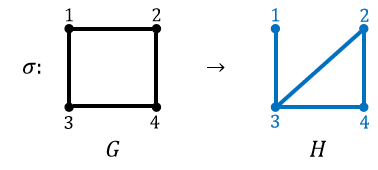
\includegraphics[width=5cm]{6-1.png}
        \caption{Symmetric difference: $|E(G)\ \Delta \ E(\sigma(G))| = 2$.}
        \label{fig:6-1}
    \end{figure}
The following theorem is a famous stability theorem by \Erdos{} and Simomovits.
\begin{theorem}[\Erdos{}-Simomovits \cite{Erds1966}, 1966]{}{}\label{ESstability}
    For each $\alpha >0$, and each graph $H$ with chromatic number $\chi(H) = r+1$, there exists $n_0 = n_0(\alpha , H)$ such that the following holds for all $n \geq n_0$.
    
    Let $G$ be an $n$-vertex graph. If $G$ is $H$-free with at least $(1-\frac{1}{r})\frac{n^2}{2}-\alpha n^2$ edges. Then $G$ can be made $r$-partite by removing at most $3\alpha n^2$ edges.
    In particular, $\Delta(G,T_{n,r}) \leq 7\sqrt{\alpha}n^2$.
\end{theorem}

Here will give another proof of Theorem \ref{ESstability} deriving from a stronger phenomenon which called perfect stability. This is a nice observation from Zolt\'an F\"uredi. He discovered that we can actually use the degree  majorization like maximum degree argument, the second proof we use for Mantel's theorem \ref{Mantel thm}. We can extend that argument to prove perfect stability statement, which then we can give a short proof of \Erdos{}-Simomovits theorem.

\begin{exercise}
    Prove the "In particular" part in Theorem \ref{ESstability}.
\end{exercise}

\begin{exercise}
    Let $K=K_{n_1, n_2, \dots, n_r}$ be an $n$-vertex complete $r$-partite graph with $e(K) \geq e(T_{n,r}) -2t$ for some $t$. Show that $$\sum\limits_{i=1}^{r} (n_i - \frac{n}{r})^2 \leq 4t$$ and $$\Delta(K,T_{n,r}) \leq 2n\sqrt{\frac{t}{r}}.$$
\end{exercise}
This exercise also shows that if a complete $r$-partite graph has size approximately equal to $T_{n,r}$, then its partite size is approximately equal to $\frac{n}{r}$.

\subsubsection{Perfect stability for \Turan{} problem}
\begin{theorem}[F\"uredi \cite{Fredi2015proof}, 2015]{}{}\label{furdedi-perfect-stability}
    Let $t\in\mathbb{N}$ and $G$ be an $n$-vertex $K_{r+1}$-free graph with $e(T_{n,r}) - t$ edges. Then $G$ can be made $r$-partite by removing at most $t$ edges. That is, there exists a subgraph $G' \subseteq G$ with at least $e(G) - t$ edges and chromatic number at most $r$.

    Furthermore, there exists a complete $r$-partite graph $K$ with $V(K)=V(G)$ such that $\Delta(G,K) \leq 3t$.
\end{theorem}

\begin{exercise}
    Prove the "Furthermore" part in Theorem \ref{furdedi-perfect-stability}.
\end{exercise}

\begin{remark}
    $\bullet$ The perfect stability does not have $\alpha >0$ or some $n_0$, it works for all $n$ and $t$. In particular, when $t = 0$, F\"uredi's theorem implies the \Turan{} theorem.

    $\bullet$ It gives a linear relation between the edit-distance $\Delta(G,K)$ and $e(T_{n,r}) - e(G)$.
\end{remark}

The proof of F\"{u}redi uses the \Erdos{}'s degree majorization argument that we used in the second proof of Mantel's theorem and \Turan{}'s theorem.

\begin{proof}[Proof of Theorem \ref{furdedi-perfect-stability}]{}{}
    It suffices to find a partition $V(G)=V_1\cup \cdots \cup V_r$ such that the number of inner edges $\sum\limits_{i=1}^{r} e_{G}(V_i)\leq t$.

    Pick a vertex $x_1\in V(G)$ with maximum degree. Let $V_1 = V \backslash N(x_1)$ and $\overline{V}_1= N(x_1)$. 
    For any $x \in V_1$, $d(x) \leq d(x_1) = |\overline{V}_1|$. Double count the degree sum of $V_1$, we have 
    \begin{equation*}
    |V_1||\overline{V}_1|\geq \sum\limits_{x\in V_1} d(x) = e_{G}(V_1,\overline{V}_1) +2 e_{G}(V_1).
    \end{equation*}

    Then zoom into $\overline{V}_1$ and repeat this process: In general, let $\overline{V}_0=V(G)$. For every $i \geq 1$, pick a vertex $x_i$ with maximum degree in $G[\overline{V}_{i-1}]$. Let $V_i=\overline{V}_{i-1}\backslash N(x_i)$ and $\overline{V}_i=\overline{V}_{i-1}\cap N(x_i)$.
    \begin{figure}[htbp]
        \centering
        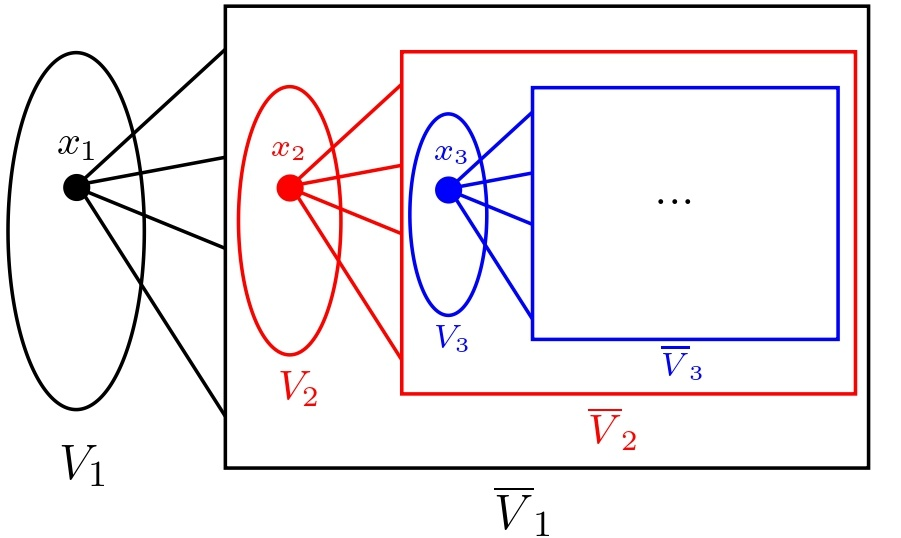
\includegraphics[width=5cm]{6-2.png}
        \caption{An illustration of the proof for Theorem \ref{furdedi-perfect-stability}}
        \label{fig:6-2}
    \end{figure}

     By the choice of $x_i$, $d(x,\overline{V}_{i-1})\leq |\overline{V}_i|$ for each $x_i \in V_i$.

     Therefore, \begin{equation}\label{equ6-1}
         |V_i||\overline{V}_i|\geq \sum\limits_{x\in V_i} d(x,\overline{V}_{i-1}) = e_G(V_i,\overline{V}_i) +2 e_G(V_i).
     \end{equation}

     At the end of the process, we get a partition $V=V_1\cup \cdots \cup V_s$ for some $s \in \mathbb{N}$. Note that $s\leq r$ as $x_1,\dots,x_s$ form a clique and $G$ is $K_{r+1}$-free. 

     Summing up (\ref{equ6-1}), we have
     \begin{equation*}
         e(T_{n,r})\geq e(K_{|V_1|,\ldots,|V_s|})=\sum\limits_{i=1}^{s} |V_i||\overline{V}_i|\geq \sum\limits_{i=1}^{s} (e_G(V_i,\overline{V}_i) +2 e_G(V_i))=e(G)+\sum\limits_{i=1}^{s} e_G(V_i).
     \end{equation*}

     Thus, \begin{equation*}
         \sum\limits_{i=1}^{s} e_G(V_i)\leq e(T_{n,r})-e(G)=t.
     \end{equation*}
\end{proof}

Here will give some recent works on stability.

Mubayi (\cite{Mubayi2006AHE}, 2006) shows that the degree majorization argument of \Erdos{} is also useful for hypergraph problems.
Liu, Pikhurko, Sharifzadeh and Staden (\cite{Liu2020StabilityFG}, 2020) presented an  axiomatic proof giving a sufficient condition to guarantee perfect stability, applied to the indubitability problem. 
Balogh, Clemen, Lavrov, Lidick\'y and Pfender (\cite{Balogh2019MakingKG}, 2019) gave a bound for the relationship of $\alpha$ and $\epsilon$ in the \Erdos{}–Simonovits stability theorem which is asymptotically sharp as $\epsilon\to 0$.
Xizhi Liu, Mubayi and Reiher (\cite{Liu2021AUA}, 2021)  presented a method which provides a unified framework for most stability theorems that have been proved in graph and hypergraph theory, reducing stability for a large class of hypergraph problems to the simpler question of checking that a hypergraph $H$ with large minimum degree that omits the forbidden structures is vertex-extendable. 

\begin{definition}
    Let $\mathcal{G}$ be a graph family and $\lambda$ be a parameter defined on members of $\mathcal{G}$.
    We say $\lambda$ is $perfectly$ $stable$ if there exists a constant $C>0$ such that for any graph $G \in \mathcal{G}$ of order $n$, there exists a complete multipartite graph $K$ of order $n$ such that $$\Delta (G, K) \leq C(\lambda(n)-\lambda(G)).$$ 
    Where $$\lambda(n) = \max \{\lambda(G): G \in \mathcal{G}, |G|=n\}.$$
\end{definition}
\begin{remark}
    Fr example, $\mathcal{G}$ is a family of all $K_{r+1}$-free graphs. $\lambda(G) = e(G)$ for all $G \in \mathcal{G}$. Then the definition above is one way of stating perfect stability in abstract setting. So, some possible direction of research is to discover the perfect stability in other setting or discrete structure.
\end{remark}

\subsubsection{\Erdos{}-Simonovits stability from perfect stability}
\begin{lemma}[Ruzsa-Szemer\'edi Removal Lemma \cite{Ruzsa1978Triple}, 1978]\label{RS-Removal lemma}
For any $\alpha >0$ and a graph $H$ with $\chi(H)=t$, there exist $n_0=n_0(\alpha,H)$ such that the following holds for all $n\geq n_{0}$. 
Let $G$ be an $n$-vertex $H$-free graph.
Then $G$ contains a $H$-$hom$-free subgraph $G'$ with $e(G')\geq e(G)-\alpha n^{2}$. In particular, $G'$ is $K_t$-free.
\end{lemma}

\begin{proof}[Proof of Theorem \ref{ESstability}]{}{}
    Applying Lemma \ref{RS-Removal lemma} on $G$, we get a $K_{r+1}$-free subgraph $G_1 \subseteq G$ with $$e(G_1)\geq e(G)-\alpha n^{2} \geq e(T_{n,r})-2\alpha n^{2}.$$

    By perfect stability (Theorem \ref{furdedi-perfect-stability}) with $t=2\alpha n^{2}$, $G_1$ can be made $r$-partite by removing at most $2\alpha n^{2}$ edges. That is, there exists an $r$-partite subgraph $G_2\subseteq G_1$ with $$e(G_2) \geq e(G_1) -t \geq e(G)-3\alpha n^{2}.$$ So $G$ can be made $r$-partite by removing at most $3\alpha n^{2}$ edges.
\end{proof}

\subsection{Stability Method}
One way of using the stability result is to boost an asymptotic solution to an exact one, so called stability method.

Usually we tackle an extremal problem as the following steps.
\begin{itemize}
    \item \textbf{Step 1:} Obtain asymptotic result;

    \item \textbf{Step 2:} Obtain stability result;

    \item \textbf{Step 3:} Use the structural information from the stability to slowly remove imperfection to get an exact result.
\end{itemize}

As an illustration, we prove the following special case of Colon-Critical graph.

\begin{theorem}{}{}\label{6-illustration}
    ${\rm ex}(n,C_{2k+1})=\lfloor\frac{n^2}{4}\rfloor = {\rm ex}(n,K_3).$
\end{theorem}

\textbf{Step 1} is provided by \Erdos{}-Stone-Simonovits theorem (Theorem \ref{ESS}). That is, ${\rm ex}(n,C_{2k+1})= \frac{n^2}{4} + o(n^2)$. \textbf{Step 2} is provided by \Erdos{}-Simonovits stability (Theorem \ref{ESstability}). It remains to show the last one.

\begin{lemma}
    Let $\alpha >0$, there exists $n_0$ such that the following holds for $n\geq n_0$.
    Let $G$ be an $n$-vertex $C_{2k+1}$-free graph. If $e(G)\geq \frac{n^2}{4}-\alpha n^2$, then $G$ can be made bipartite by removing at most $3\alpha n^2$ edges.
\end{lemma}

\begin{proof}[Proof of Theorem \ref{6-illustration}]
\textbf{Idea: } For the lower bound, the complete bipartite graph is enough. 

For the upper bound: Take a max-cut $X\cup Y$ which minimized the inner edges and maximized the crossing edges between $X$ and $Y$. It suffices to show that $e_G(X) + e_G(Y) = 0$. Firstly we will show that $|X| + |Y| \approx \frac{n}{2}$. Then we will show a weaker property that the maximum inner degree is $o(n)$. Finally not a single edge is allowed.
    
\end{proof}

\newpage
\section{Lecture 7}
\subsection{Extremal Number of $\boldsymbol{C_{2k+1}}$ via Stability Method}

Initially, let's review the process to tackle an extremal problem.

\begin{itemize}
    \item \textbf{Step 1:} Obtain asymptotic result;
 
    \item \textbf{Step 2:} Obtain stability result;
    
    \item \textbf{Step 3:} Use the structural information from the stability to slowly remove imperfection to get an exact result.
\end{itemize}

As an illustration, let's prove theorem \ref{6-illustration}, the special case of color-critical graph, which we mention in last lecture,
$$ex(n,C_{2k+1})=\left \lfloor \frac{n^2}{4} \right \rfloor = ex(n,K_3).$$

Before we prove theorem \ref{6-illustration}, let's give a theorem we will use.
\begin{theorem}[\Erdos{}-Gallai \cite{1959On}]\label{EG}
    $ex(n,P_t) \le \frac{t-2}{2}n$
\end{theorem}
\begin{remark}
    This is optimal, when $(t-1)|n$. A graph is an extremal graph, when all its components are complete graphs of order t-1.
\end{remark}

\begin{proof}[proof of theorem \ref{6-illustration}]
Let $G_{ex}$ be an $N$-vertex extremal $C_{2k+1}$-free graph. 
\begin{itemize}
    \item \textbf{The lower bound of $\boldsymbol{e(G_{ex})}$}
\end{itemize}
According to the extremal graph of $ex(n,K_3)$, we can easily see that 
$$ex(G_{ex}) \ge \left \lfloor \frac{N^2}{4} \right \rfloor.$$
\begin{itemize}
    \item \textbf{The upper bound of $\boldsymbol{e(G_{ex})}$}
\end{itemize}

Let's find a subgraph $G \subset G_{ex}$ satisfying $\delta(G) \ge (\frac{1}{2}-\epsilon)|G|$. And we aim to bound the upper bound of $e(G_{ex})$ by counting the $e(G)$ and the edges we lost, when we definite the $G$. And we gain $G$ by doing the following process to graph $G_{ex}$.
\begin{itemize}
    \item[*] \textbf{Step 1:} Let $i=0,~G_i=G_{ex}$ and $\epsilon > 0$.

    \item[*] \textbf{Step 2:} Determine whether there exist vertex $v_i \in V(G_i)$ with $d_G(v)<(\frac{1}{2}-\epsilon)|G_i|$. If yes, proceed to next step; if not, stop and output $G$.
    
    \item[*] \textbf{step 3:} Let $i=i+1$, define $G_i=G_{i-1}-v$ and return to step 2.
\end{itemize}

\begin{claim}\label{claimofprcess}
    this process must terminate with a desired graph $G_k=G$.
\end{claim}

\begin{proof}
According to process, let's count the edges in Graph $G$.
\begin{align*}
e(G_k) \ge \frac{N^2}{4}-\sum_{i=1}^{k}(\frac{1}{2}-\epsilon)(N+1-i) \ge \frac{N^2}{4}-(\frac{1}{2}-\epsilon)Nk+(\frac{1}{2}-\epsilon)\sum_{i=1}^{k}(i-1)
\end{align*}
Write $n=|G_k|=N-k$, we gain that
\begin{align*}
e(G_k) \ge \frac{(n+k)^2}{4}-(\frac{1}{2}-\epsilon)(n+k)k+(\frac{1}{2}-\epsilon)\sum_{i=1}^{k}(i-1) = \frac{n^2}{4}+\epsilon nk + \frac{\epsilon}{2}k^2+O(k).
\end{align*}
When $k=\Omega(N)=\Omega(n)$, we have that $e(G_k) \ge \frac{n^2}{4}+\Omega(n^2)$. The result have a contradiction with the \Erdos{}-S\'os-Simonovits Theorem(Theorem \ref{ESS}). So we are able to gain the graph $G$ with the minimal degree condition.
\end{proof}

Due to the claim \ref{claimofprcess} we have graph $G \subset G_{ex}$ satisfying that Graph $G$ is $C_{2k+1}$-free and $\delta(G) \ge (\frac{1}{2}-\epsilon)n$. Therefore, the edges of graph $G$ is more than $(\frac{n^2}{4}-\frac{\epsilon}{2}n^2)$. Then let's consider the good properties of $G$.

Let $X \cup Y$ be the Max-cut for $G$. Apply \Erdos{}-Simonovits Stability Theorem(Theorem \ref{ESstability}) on $G$, we obtain 
$$e_G(X)+e_G(Y) \ge \frac{3\epsilon}{2}n^2.$$
Besides, we can obtain some good properties of Max-cut $X \cup Y$ for $G$ as follows.

\begin{claim}\label{XYsize}
    $|X|+|Y| = \frac{n}{2} \pm 2\sqrt{\epsilon}n.$
\end{claim}

\begin{proof}
Without loss generation, let's assume that $|X| \ge \frac{n}{2} + 2\sqrt{\epsilon}n$. then, we have
\begin{align*}
e(G) \le |X||Y|+e_G(X)+e_G(Y)
\le \frac{n^2}{4}-4\epsilon n^2+\frac{3\epsilon}{2}n^2 < \frac{n^2}{4}-\frac{\epsilon}{2}n^2.
\end{align*}
This contradicts the lower bound of $e(G)$.
\end{proof}

\begin{claim}\label{MaxDegree}
    $\Delta(G[X]),\Delta(G[Y]) \le 2\sqrt{\epsilon}n$.
\end{claim}

\begin{proof}
By reduction to absurdity, if there exists a vertex $x \in X$ with $d(x,X) > 2\sqrt{\epsilon}n$. $X \cup Y$ is the Max-cut of graph $G$, then $d(x,Y) \ge d(x,X) > 2\sqrt{\epsilon}n$. Let's denote $X'=N(x,X),Y'=N(x,Y)$. As $G$ is $C_{2k+1}$-free, we get that $G[X',Y']$ is $P_{2k}$-free. By the \Erdos{}-Gallai Theorem(Theorem \ref{EG}), we count the edges of $G$,
\begin{align*}
e(G) &\le \frac{3\epsilon}{2}n^2 +|X||Y|-(|X'||Y'|-kn) \le \frac{3\epsilon}{2}n^2 + \frac{n^2}{4}+kn-4 \epsilon n^2 < \frac{n^2}{4}-\frac{\epsilon}{2}n^2.
\end{align*}
This result makes a contradiction with the lower bound of $e(G)$.
\end{proof}

According to the properties of Max-cut $X \cup Y$ of $G$, let's show that there is no edge in $X$ or $Y$. By reduction to absurdity, let's suppose $u,v$ in X form an edge. And due to the properties of Graph $G$, we get
\begin{align*}
d(x,Y) \ge \delta(G)-\Delta(G[X]) \ge (\frac{1}{2}-\epsilon)n-2\sqrt{\epsilon}n \ge (1-10\sqrt{\epsilon})|Y|.
\end{align*}
According to the inequation, we know that almost full vertices in $Y$ are the neighbors of $x$ which is an arbitrary vertex of $X$. therefore, let's pick arbitrary $w_1,...,w_{k-1} \in X-\{u,v\}$. The number of common neighbors of $u,v,w_1,...,w_k$ is large,
$$|N(u) \cap N(v) \cap N(w_1) \cap...\cap N(w_{k-1})| \ge (1-(k-1)10\sqrt{\epsilon})|Y| \ge 3.$$
Thus, we can find a copy of $C_{2k+1}$ in $G$, and this contradicts our purpose. So, $G$ is bipartite graph with partition $X \cup Y$. If we delete vertex in graph $G_{ex}$ and $|G| < |G_{ex}|$, then we can bound the upper bound of $e(G_{ex})$,
\begin{align*}
e(G_{ex}) \le e(G) + \underset{i=n+1}{\overset{N}{\sum}}(\frac{1}{2}-\epsilon)i< \frac{N^2}{4}.
\end{align*}
This contradicts the lower bound of $e(G_{ex})$. Therefore, $G_{ex}$ must be graph $G$. So $G_{ex}$ is a bipartite graph and also is a homeomorphism of $T_{N,2}$.
\end{proof}

\subsection{Andrasfai-\Erdos{}-S\'os Theorem}
Let's consider this claim, For arbitrary $n$-vertex triangle-free graph $G$,if $\delta(G) > \frac{2n}{5}$, then the graph G must be bipartite. This claim is true. And the $n$-vertex graph $G$ with $n|5$ is the optimal case, when $G = C_5(\frac{n}{5})$. In this case, $\delta(G)=\frac{2n}{5}. $Meanwhile, this claim is a special case of the following theorem.

\begin{theorem}[Andrasfai-\Erdos{}-S\'os \cite{ANDRASFAI1974205}]\label{AES}
For arbitrary $n$-vertex $K_r$-free graph $G$, if $\delta(G) > \frac{3r-7}{3r-4}n$, then $G$ is an $(r-1)$-partite graph.
\end{theorem}
\begin{remark}\label{TightBdofAES}
There exist two cycles $C_5$ and $C_{r-3}$. For $\forall v \in C_5$, it is adjacent with each $u \in C_{r-3}$. Then, let's blow $\forall v \in C_5$ up to $V$ with $|V|=\frac{n}{3r-4}$ and blow $\forall u \in C_{r-3}$ up to $U$ with $|U|=\frac{3n}{3r-4}$. As is shown in the following figure.
    \begin{figure}[htbp]
	\centering
	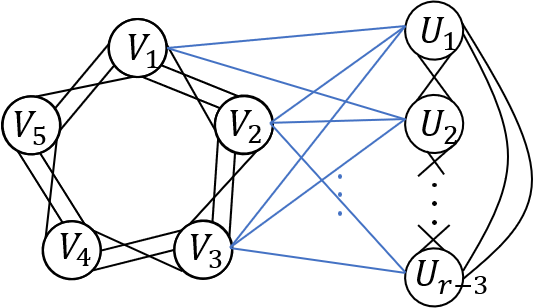
\includegraphics[width=5cm]{7-1.png}
        \caption{The optimal graph with $\delta(G) = \frac{3r-7}{3r-4}n$}
	\label{fig:7-1}
    \end{figure}

And this graph show that the bound of theorem \ref{AES} is tight.
\end{remark}
We will give a short proof of Andrasfai-\Erdos{}-S\'os heorem(Theorem \ref{AES}) by Brandt \cite{article}, but before we do that, let's give a definition.

\begin{definition}[5-wheel-like graph $W_{r,k}$]
Given $0\le k \le r-3$ and $(2r-k-1)$-vertex graph $G$. Let's fix three vertices $v,w_1,w_2$ in graph $G$. For the residual vertices, we have $Q_1 \cup Q_2 = G-\{v,w_1,w_2\},~|Q_1|=|Q_2|=r-2$ and $|Q_1\cap Q_2|=k$. If $G$ just has the following adjacency relationship, we call it 5-wheel-like graph $W_{r,k}$.
\begin{itemize}
    \item[*] $v$ is adjacent with all vertices in $Q_1 \cup Q_2$,
    \item[*] $Q_i$ is an $(r-2)$-clique for $i=1,2$,
    \item[*] $w_1$ is adjacent with $w_2$,
    \item[*] $w_i$ is adjacent with all vertices in $Q_i$ for $i=1,2$.
\end{itemize}

\end{definition}
\begin{example}
The structure of $W_{3,0},~W_{4,0},~W_{4,1}$ is shown in the below pictures.
    \begin{figure}[htbp]
        \centering
        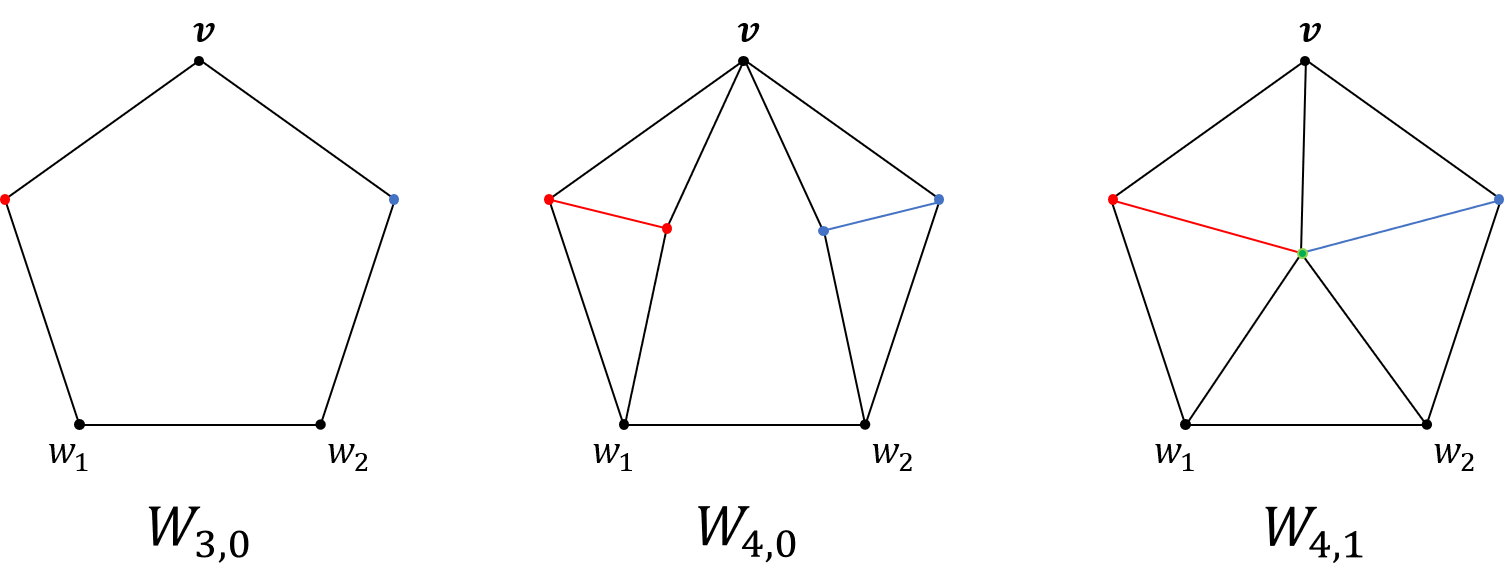
\includegraphics[width=8cm]{7-2.png}
        \caption{Some examples of $5$-wheel-like graph}
        \label{fig:7-2}
    \end{figure}
\end{example}

\begin{exercise}\label{IdeaOrigin}
Every non-bipartite maximal triangle-free graph contains a 5-cycle.
\end{exercise}

The nice idea of Brandt is generalizing the exercise \ref{IdeaOrigin}. The details are as follows.

\begin{lemma}\label{BrandtIdea}
    Arbitrary graph $G$ is maximal $K_r$-free and is not $(r-1)$-partite, then $G$ contains a $5$-wheel-like graph.
\end{lemma}

\begin{proof}
Let's suppose that $G$ is complete multipartite graph. As $G$ is $K_r$-free,  the number of partitions is at most $r-1$. However, it make a contradiction, because $G$ can't be $(r-1)$-partite. Thus, G is not complete multipartite.

Obviously, non-acjacency relation is not an equivalence relation in Graph $G$. Therefore, $G$ contains three vertices, we denote these as $\{v,w_1,w_2\}$, and $vw_i \notin E(G),~w_1w_2 \in E(G)$. As $G$ is maximal $K_r$-free, $N(v) \cap N(w_i)$ contains a copy $Q_i$ of $K_{r-2}$ for each $i=1,2$. Otherwise, $G+vw_i$ is still $K_r$-free. This contradicts maximality of $G$. Then, there is a copy of $5$-wheel-like graph $W_{r,k}$ in the induced subgraph $G[Q_1 \cup Q_2 \cup \{v,w_1,w_2\}]$. 
\end{proof}

\begin{proof}[Proof of Andrasfai-\Erdos{}-S\'os Theorem \ref{AES}]
By adding edges if necessary, we may assume $G$ is maximal $K_r$-free. By the Lemma \ref{BrandtIdea}, $G$ contains $W_{r,k}$. Let's pick a copy $W$ of $W_{r,k}$ with maximum value $k$. Define $X$ is the common neighbors of $Q_1 \cap Q_2$, we will bound $|X|$ in two ways.

As G is $K_r$-free and $W$ contains a $K_{r-1}$, we get that for arbitrary vertex $v$, $v$ is not completely joined to $W$. Write $p=|W|$, we have
$$d(v,W) \le p-1.$$
\begin{claim}
    For arbitrary $x \in X$, $d(x,W) \le p-3$.
\end{claim}

\begin{proof}
$G$ is $K_r$-free, so $x$ has a non-neighbor in $Q_i \cup v$ and $Q_i \cup w_i$ for $\forall i \in [2]$. Let assume $vx \in E(G)$. By the above observation, $x$ has a non-neighbor $y_1 \in Q_1\backslash Q_2,~y_2 \in Q_2 \backslash Q_1$, we denote $Q'_i=Q_i-y_i+x$. Consider $v,w_1,w_2,Q'_1,Q'_2$, we get $W_{r,k+1}$. This is contradicts maximality of $k$ in $W_{r,k}$. Therefore, $vx \notin E(G)$ and $d(x,W) \le p-3$.
\end{proof}
Similarly, $x$ has non-neighbor in disjoint $Q_i \cup w_i \backslash (Q_1 \cap Q_2)$. Let's calculate the degree sum of $W$ by double counting,
\begin{align}\label{1}
p\delta(G) \le {\underset{w\in W}\sum}d(w) \le (p-3)|X|+(p-1)(n-|X|).
\end{align}
On the other hand, by pigeonhole principle, as X is the common neighbors of $Q_1 \cap Q_2$. We have 
\begin{align}\label{2}
	|X| \ge k\delta(G)-(k-1)n.
\end{align}
Compare with \eqref{1} and \eqref{2}, we get
$$\delta(G) \le \frac{2r+k-4}{2r+k-1}n \le \frac{3r-7}{3r-4}n.$$
It contradicts the degree condition. So $G$ is an $(r-1)$-partite graph.
\end{proof}

\begin{remark}
    By the Andrasfai-\Erdos{}-S\'os Theorem(Theorem \ref{AES}), when an n-vertex triangle-free Graph has condition $\delta(G) > \frac{2n}{5}$, Graph $G$ is a bipartite and $\chi(G) \le 2$.
\end{remark}

Naturally, we can ask the following question.

\begin{question}
    How much can we reduce minimal degree, if we only require to bound lower bound of the number of chromaticity $\chi(G)$.
\end{question}

\subsection{Extensions}
\begin{definition}
    $ex(n,\Gamma,H)$ is the maximal number of the copies of $\Gamma$ in an $n$-vertex $H$-free graph.
\end{definition}
\begin{remark}
     Obviously, \Turan{} problem is a special case of $ex(n,\Gamma,H)$, i.e. $ex(n,H) = ex(n,K_2,H)$. Besides, There also have some results of this question.
\begin{itemize}
    \item \Erdos{}\cite{MR0151956} solved the clique case: For $\forall s < t,~ex(n,K_s,K_t)$ is maximized by $T_{n,t-1}$.
    \item In 2016, N. Alon and C. Shikhelman\cite{ALON2016146} got three representative result:
	\\ 1) $ex(n,K_3,C_5) \le (1+o(1))\frac{\sqrt{3}}{2}n^{3/2}$,
	\\ 2) For any fixed $m,~s \le 2m-2$ and $t \le (s-1)!+1$, $ex(n,K_m,K_{s,t})=\Theta(n^{m-\binom{m}{2}/s})$,
	\\ 3) For any two trees $H$ and $T$, $ex(n,T,H)=\Theta(n^m)$, where $m=m(T,H)$ is an integer depending on $H$ and $T$.
    \item In 2018, L. Gishboliner and A. Shapira \cite{inproceedings} got that:
\begin{align*}
	ex(n,C_k,C_l)=\left\{
	\begin{array}{llllllllll}
		{\Theta_k(n^{k/2})} & {k \ge 5,~l=4,} \\
		{\Theta_k(l^{\left\lceil k/2 \right\rceil}n^{\left\lfloor k/2 \right\rfloor}} & {l\ge 6~\text{even,} k\ge 4,}\\
		{\Theta_k(l^{\left\lceil k/2 \right\rceil}n^{\left\lfloor k/2 \right\rfloor}} & {k,l~\text{odd},~5\le k <l.}
	\end{array}\right.
\end{align*}
    \item In 2011, Grzesik \cite{Grzesik2011OnTM} and H. Hatami, J. Hladký et al \cite{HATAMI2013722} got that $ex(n,C_5,K_3) \le (\frac{n}{5})^5$
\end{itemize}
\end{remark}
Below are \Erdos{}'s two conjectures for $250$ dollars.
\begin{conjecture}[sparse halves \cite{ERDOS198881}]
    Arbitrary n-vertex triangle-free graph $G$ contains a set of $\frac{n}{2}$ vertexs inducing at most $\frac{n^2}{50}$ edges.
\end{conjecture}
\begin{remark}
If the conjecture is true. The $n$-vertex graph $G$ with $n|5$ is the best possible, when $G = C_5(\frac{n}{5})$.
\end{remark}

\begin{conjecture}[\cite{ERDOS198881}]
    Arbitrary n-vertex triangle-free graph $G$ can be made bipartite by removing at most $\frac{n^2}{25}$ edges.
\end{conjecture}


\newpage
\section{Lecture 8}
We first recall the famous \Erdos{}-Stone-Simonovits theorem, is the following.
\begin{theorem}[\Erdos{}-Stone-Simonovits Theorem \cite{erdos1966limit, erdos1946linear}, 1946]{}{} \label{ESS}
    For any fixed graph $H$ and any fixed $\epsilon >0$, there is $n_0$ such that, for any $n\leq n_0$,
    $$ \ex(n,H)\leq (1-\frac{1}{\chi(H)+1}+o(1))\frac{n^2}{2}.$$
\end{theorem}
For the bipartite graph $H$, the \Erdos{}-Stone-Simonovits theorem gives $\ex(n,H)=o(n^2)$. Actually, for any bipartite graph $H$, $\ex(n,H)=o(n^{2-c_H})$ where $c_H$ is a constant. \par
In this lecture, we focus on the bipartite \Turan{} problem. We mainly consider even cycle and the complete bipartite graph. In \Cref{8.1}, we focus on  the \Turan{} number of even cycle.  In \Cref{8.2}, we talk about the  \Turan{} number of complete bipartite graph. In \Cref{8.3}, we give some applications of the bipartite \Turan{} problem. 


\subsection{\Turan{} problem of even cycle}\label{8.1}

\begin{theorem}[Balogh-Jozsef \cite{MR2680230},2024]\label{c4}
    $\ex(n,C_4)\leq \frac{n}{4}(1+\sqrt{4n-3})=(\frac{1}{2}+o(1))n^{\frac{3}{2}}.$
\end{theorem}

\begin{proof}
    Let $G$ be an $n$-vertex $C_4$-free graph. Denote the number of $K_{1,2}$'s in $G$ by $t$. We are going to double count $t$. On the one hand, the number of $K_{1,2}$ is given by  
    $$t={\underset{v\in V(G)}\sum} \binom{d(v)}{2}\geq n\binom{\frac{1}{n}\underset{v\in V(G)}\sum d(v)}{2}=n\binom{\frac{1}{n}2e(G)}{2}=\frac{2e(G)^2}{n}-e(G),$$
    where the first inequality holds by Jensen's inequality: if $f$ is convex, then for all random variable $X$ we have $\mathbb{E}(f(X))\geq f(\mathbb{E}X)$.\par
    
    On the other hand, no two vertices share the same two neighbors, otherwise there will be a $C_4$. Hence,
    $$t\leq \binom{n}{2}.$$\par
    Then $e(G)\leq \frac{n}{4}(1+\sqrt{4n-3})=(\frac{1}{2}+o(1))n^{\frac{3}{2}}.$
    \end{proof}
Note that $C_4=K_{2,2}$. By double counting $K_{1,t}$ instead of $K_{1,2}$ we get the following.
\begin{exercise}\label{kstg}
    Let $s\leq t$ be two integers, $\ex(n,K_{s,t})\leq tn^{2-\frac{1}{s}}.$
\end{exercise}

\begin{theorem}[\Erdos{}-R\'enyi-S\'os \cite{MR0159319}, 1963]
     $\ex(n,C_4)\geq (\frac{1}{2}+o(1))n^{\frac{3}{2}}.$
\end{theorem}
\begin{proof}
    For large enough $n$, there is a prime number $p$ between $(1+o(1)\sqrt{n+1}$ and $\sqrt{n+1}$. Let $G=(V(G),E(G))$ with $V(G)=\mathbb{F}_p^2\backslash\{(0,0)\}$ and $E(G)=\{(a,b)\sim (x,y):ax+by=1\}$. Every vertex in $G$ has degree $p$ or $p-1$.
Hence, 
$$e(G)\geq \frac{1}{2}(p-1)(p^2-1)=(\frac{1}{2}-o(1))n^{\frac{3}{2}}.$$\par
Take two distinct vertices $(a_i,b_i)$, $i\in [2]$. Let $N((a_i,b_i))$ consists of all vertex $(x,y)$ satisfying $a_ix+b_iy=1$(line in $\mathbb{F}_p^2$). As $(a_i,b_i)\neq (a_2,b_2)$, $N((a_1,b_1))$ and $N((a_2,b_2))$ are two different lines which can intersect at most one point.
Hence, $(a_1,b_1)$ and $(a_2,b_2)$ have at most one common neighbor which means $G$ is $C_4$ free.
\end{proof}
A related problem asked by Fischer and Matousek(\cite{fischer2001lower} , 2021).
\begin{problem} \label{ct}
    Let  $G$ be a $3$-partite graph with vertex set $(V_1,V_2.V_3)$ where $|V_1|=|V_2|=|V_3|=n$. And the induced graphs $G[V_1,V_2]$, $G[V_1,V_2]$ and $G[V_1,V_2]$ are $C_4$-free. Then what is the maximum number of triangles in $G$?
\end{problem}

The known result of Problem  \ref{ct} is $\Omega(n^{\frac{5}{3}})\leq \# traingles \leq \Omega(n^{\frac{7}{4}})$. And the lower bound is given by Coulter-Mathlhews-Timmons.





\begin{theorem}[Bondy-Simonovits \cite{bondy1974cycles}, 1974] \label{bstc}
    $\ex(n,C_{2k})= O(n^{1+\frac{1}{k}}).$
\end{theorem}

\begin{remark}
    For $k=2,3,5$, some finite geometry constructions can match the lower bound in theorem \ref{bstc}. For $k=4$, it still open. And the known result is $\Omega(n^{\frac{6}{5}})\leq \ex(n,C_8)\leq O(n^\frac{5}{4})$. The lower bound is given by Lazebuik-Ustimenko-Wolder(\cite{lazebnik1999polarities}, 1999).  
\end{remark}



\begin{theorem}[Pikhurko \cite{pikhurko2012note}, 2012] \label{pt}
    For large $n$, $\ex(n,C_{2k})\leq 4kn^{1+\frac{1}{k}}$.
\end{theorem}

\begin{remark}
    The best leading constant in \Cref{pt} is $O(\sqrt{k\log k}n^{1+\frac{1}{k}})$(\cite{thomassen2007chromatic}, 2002).
\end{remark}

Open problem: Is $\ex(n,C_{2k})=o(\sqrt{k}\cdot n^{1+\frac{1}{k}})$ ?\par

To warm up, let us consider forbidding $\mathcal{C}_{2k}:=\{C_4,C_6,\cdots,C_{2k}\}$. We try to show that $\ex(n,\mathcal{C}_{2k})=O(n^{1+\frac{1}{k}})$. Suppose $G$ is a $\mathcal{C}_{2k}$-free graph with $n$ vertices. Take a BFS(Breadth First Search), then we have a tree $T$ rooted at some $x\in V(G).$ Let $V_i=\{v\in V(G)|dist(v,x)=i\}$. For each $i\leq k$, as $G$ is $\mathcal{C}_{2k}$-free, we know that every vertex $v\in V_i$ has a unique father in $V_{i-1}$ It follows that $|V_i|\geq \delta(G)^i$. Then, $\delta(G)^k\leq |V_k|\leq|V(G)|=n$. This conclusion follows from $\delta(G)\leq n^{\frac{1}{k}}$.

\begin{remark}
    We have to be more careful to implement this BFS approach as now we only forbidding $C_{2k}$. Note that $C_{2i}$ is a degenerate homomorphic image of $C_{2k}$ for each $i\leq k$. The main difficulty in many bipartite \Turan{} problem is to control the count of such degenerate homomorphisms.
\end{remark}










\begin{proposition}
    For any graph $G$, $G$ contains a subgraph $H$ with $\delta(H)\geq \frac{d(G)}{2}$.
\end{proposition}

\begin{proposition}
    For any graph $G$, $G$ contains a bipartite subgraph $H$ with $e(H)\geq \frac{e(G)}{2}$.
\end{proposition}

\begin{definition}
    A $\Theta_k$-graph is a cycle of length at least $2k$. with a chord.
\end{definition}

\begin{exercise}
    Let $k\geq 3$ and $H$ be a bipartite graph with $d(H)>2k$. $H$ contains a $\Theta_k$-graph.
\end{exercise}

The idea of the proof of \Cref{pt}: Consider a BFS tree T. If between any of the first $k$
pairs of consecutive layers, there is a $\Theta_K$-graph, then there will be a $C_{2k}$. There is a contradiction. So, there is no $\Theta_K$-graph between any of the first $k$ pairs of consecutive layers.
By Exercise 10.18, the average degree between every pair of consecutive layers is less than $2k$. Then each of the first $k$ layers expands by a factor of $\Omega(\frac{d(G)}{k})$.\par
Now, we need the following lemma, showing that every  $\Theta_K$-graph contains many paths of varying length.

\begin{lemma}
    Let $F$ be a $\Theta_k$-graph and let $A\cup B=V(F)$ be a non-trivial partition ($A,B\neq \emptyset$). If $F$ is not bipartite with bipartition $A\cup B$, then there is a $(A,B)-paths$ of length less than  $|F|=n$.
\end{lemma}
\begin{proof}
Suppose for some $1 <1 < n$, there is no $A, B$-path of length $l$ in $F$. We need to prove that
$F$ is bipartite with bipartition $A \cup B$.

Identify the spanning cycle in $F$ with $\mathcal{Z}_n$ and think of $(A, B)$ partition as a 2-coloring $c$ of $\mathcal{Z}_n$.


Define the set of periods of $c$ as $P= \{ m \in  \mathcal{Z}_n : \text{ For each } i \in \mathcal{Z}_n, C(i)
=c(i + m)\}$. By our
assumption, $l\in P$. The smallest period $m$ in $P$ divides $n$, otherwise we can get a smaller period $m^\prime$. This implies that $P = \{mi : i \in  \mathcal{Z}_n\}$. Otherwise we can also get a smaller period $m^\prime$. (Left as
an exercise.) Besides,$A \cup B$ is a non-trivial partition, so $m > 1$.


We may assume $m > 2$, for otherwise $A \cup B$ is a bipartition of $F$. (If the chord connect two
vertices of same color, there are $A, B$-paths of all lengths.) Suppose the chord in $F$ connect vertices
0 and $r$.


If $n-r \equiv {r} \equiv 1 \pmod {m}$, then $n = (n -r) + r \equiv 2 \pmod {m}$. This contradicts to the facts that
$m > 2$ and $m|n$.
Suppose $r \not \equiv 1 \pmod {m}$, i.e., $r-1 \notin  P = \{mi: i \in \mathbb{Z}_n\}$. As $l \in  P$, there exists some $j \in \mathcal{Z}_n$ such that $c(i) \neq c(i+ l+r- 1)$. We may assume
$-m < j < 0$, for otherwise we can rotate it.
Consider the $l$-walk
$$j,j+1,\cdots ,-1,0,r,r+1,\cdots,j+l+r-1.$$
It is an $A, B$-walk. We get a contradiction unless $l+r-1\geq n$. But we can assume $l+r-1< n$
by subtracting multiples of $m$ whiling still being a non-period.

The case $n -r \not \equiv 1 \pmod {m}$ can be handled similarly.

\end{proof}

\begin{proof}[The proof of \Cref{pt}]
 Let $G$ be a $C_{2k}$-free graph with $n$ vertices and at least $4kn^{1+1/k}$ edges. By
passing to a subgraph $H$ and losing a factor of 4, $H$ is a bipartite graph with minimum degree at
least $d(G) /4$ which is larger than $2k \cdot n^{1/k}$. For each $i > 0$, let $V_i = N^i_{H}(x)$ and $H = H[V_i, V_{i+1}]$.
   
\begin{claim}
    For each $i < k - 1$, $H_i$ has no $\Theta_k$-subgraph.
\end{claim} .

We first show that the theorem can be obtained from Claim 10.20. Exercise 10.18 implies that
$d(H_i) < 2k -1$. Iteratively, as $n \gg k$, for $i = 0,1,2,\ldots, k - 1$, on average, each vertex in $V_i$ sends downward to $V_{i+1}$ at least $\delta_(H) - O(k)$ edges, while each vertex in $V_{i+1}$ sends back to $V_i$ at most $2k-1$ edges. Then for each $0\leq i\leq k-1$, we have
$$\frac{|V_{i+1}|}{V_i}\geq \frac{\delta(H)-O(k)}{2k-1}.$$
Thus,$$ n\geq |V_k|= \frac{|V_k|}{|V_|k-1|} \frac{|V_{k-1}|}{|V_|k-2|} \cdots \frac{|V_1|}{1}\geq (\frac{\delta(H)-O(k)}{2k-1})^k.$$
Then, $\delta(H)< 2kn^{\frac{1}{k}}$. There is a contradiction. So, it remains to prove the claim.\par
Suppose that $H_i$ contains a $\Theta_k$-graph $F$
We shall find a copy of $C_{2k}$ to get a contradiction.
Notice that $F$ is bipartite. Let $Y \cup Z$ be a bipartition of $V (F)$. Let $Y_i = Y \cap V_i$, $Y_{i+1}
= Y \cap V_{i+1}, Z_i=Z \cap V_i$, and $Z_{i+1}
= Z \cap V_{i+1}$.

For a vertex $v \in T$, write $D(v)$ for its descendents. Let $y$ be a minimal ancestor of $Y_i$, that is,
$y$ is the farthest vertex from a such that $Y_i \subseteq D(y)$. Take a child $z$ of $y$ such that $A = D(z)\cup Y_i$
which is not empty. Set $Y_i\backslash A$ is not empty for the minimality of $y$.


Consider the nontrivial partition $A$ and $B = V (F)\ A$. As every vertex in $F$ has degree at least
2, there must be edges between $B\cap V_i$ and $B\cap V_{i+1}$. Then $(A, B)$ is not a bipartition of $F$. By
Lemma 10.19, there exists a $(A, B)$-path of any length less than $F$. Let $l$ be the distance between
2 and $y$. So $l < i$ and $2k -2(i-1) < 2k <|F|$. By Lemma 10.19, there exists a $a, b$-path $P$ of length
$2k-2(i-1)$ and $a\in A\subseteq Y_i$, $b \in B$. Since $P$ has even length, we know $b \in Y_i$. Besides, $(Y, Z)$ is
a bipartition. Then we construct a cycle $C_{2k}$ by combining $y$, $a$-path, $y, b$-path and $P$. There is a contradiction. This completes the proof of the claim, and thus, of the theorem.




\end{proof}





\subsection{\Turan{} problem of complete bipartite graph}\label{8.2}
A careful calculation using the approach in the proof of  \cref{c4} gives the following result.
   \begin{theorem}[K\H{o}vari-S\'os-\Turan{} \cite{kHovari1954problem}, 1954]\label{kst}
         Let $s\leq t$ be two integers, $\ex(n,K_{s,t})\leq (\frac{1}{2}+o(1))(t-1)^{\frac{1}{s}}n^{2-\frac{1}{s}}.$
    \end{theorem}
\begin{remark}
    The major open problem is the construction of the lower bound of theorem \ref{kst}.The known lower bound is $\Omega(n^{2-\frac{1}{s}})$ for $s=2,3$. For $s=t=4$, the known best result is $\Omega(n^{\frac{5}{3}})\leq \ex(n,K_{4,4})\leq O(n^{\frac{7}{4}}).$ For $t\gg s$, Kolla\'r-Ro\'nyai-Szab\', Alon-Ro\'nyai-Szab\' and Bukh also proved the lower bound $\Omega(n^{2-\frac{1}{s}})$. For other $s$ and $t$, it still open.
\end{remark}
\begin{construction}[Brown's construction]
    Let $G=(V,E)$. Let $V(G)=\mathbb{F}_p^3$, and two points $v=(a,b,c)$ and $v'=(a',b'
    ,c')$ are adjacent if and only if $||v-v'||^2=(a-a')^2+(b-b')^2+(c-c')^2=1$. It is not hard to see that the graph $G$ is $K_{3,3}$-free. Let us give a geometric intuition: $N(v)$ corresponds a sphere around $v$ and three spheres have at most two common points. 
\end{construction}
    



\subsection{Application}\label{8.3}
\subsubsection{$C_4$-free graph \& Sidon set}

\begin{definition}
    A set $S=\{a_1,a_2,\cdots,a_k\}\subseteq \mathbb{N}$ is a \textbf{Sidon set} if all pairwise sums $a_1+a_j$ are distinct. In other words, $a+b=c+d$ has only trivial solution $\{a,b\}=\{c,d\}$ in $S$.
\end{definition}
\begin{question}
    How large can a Sidon set in $[n]$ be ?
\end{question}
Consider the numbers of powers of 2: $1,2,2^2,2^3$,$\dots$,$2^k=n$. This is an example of a Sidon set of size $\log_2 n$. 

\begin{theorem}\label{SS}
    The largest Sidon set in $[n]$ has size $(1+o(1)\sqrt{n})$.
\end{theorem}

\begin{exercise}
\leavevmode
    \begin{itemize}
        \item Prove the weaker bound that for any Sidon set in $[n]$ has size at most $2\sqrt{n}$.
        \item Use the Theorem \ref{SS} to construct an $n$-vertex $C_4$-free graph with $\Omega(n^{\frac{3}{2}})$ edges.
    \end{itemize}
\end{exercise}

\subsubsection{$K_{s,t}$-free graph \& \Erdos{} unit distance problem}
\begin{proposition}\label{pd}
    A set of $n$ points in $\mathbb{R}^2$ determines $O(n^{\frac{3}{2}})$ unit distance.
\end{proposition}
\begin{proof}
    Build an auxiliary graph $G$ on these $n$ points are adjacent if the distance of two vertices is $1$. We are going to bound $e(G)$.
    Observed that $G$ is $K_{2,3}$-free. By exercise \ref{kstg}, $e(G)=O(n^{\frac{3}{2}})$.
 \end{proof}
\begin{remark}
    The best upper bound in Proposition \ref{pd} is $O(n^{\frac{4}{3}})$ by Szemer\'edi-Trotter(\cite{shkredov2015sums}, 2014).
\end{remark}

\newpage
\section{Lecture 9: Regularization}

In this section we will introduce a lemma, called regularization, which is very useful to deal with  bipartite \Turan{} problem.  

A lemma of \Erdos{}-Simonovits allows us to work with almost regular graphs for bipartite \Turan{} problem. Here, we say that a graph $G$ is $K$-\emph{almost regular} if $\Delta(G)\leq K\cdot \delta(G)$. The following lemma guarantees the existence of a $K$-almost regular graph. 

\begin{lemma}[P. \Erdos{} and M. Simonovits \cite{Erdos1969},1969]\label{regularization}
    Let $0<\varepsilon<1$, $c>0$, $K=20\cdot 2^{\frac{1}{\varepsilon^2}+1}$ and $n$ be sufficiently large. Let $G$ be an $n$-vertex graph with $e(G)\geq c \cdot n^{1+\varepsilon}$. Then $G$ contains an $m$-vertex $K$-almost regular subgraph $G^\prime$ with $m\leq n^{\frac{\varepsilon-\varepsilon^2}{4+4\varepsilon}}$ and $e(G^\prime)\geq \frac{2c}{5}m^{1+\varepsilon}$. 
\end{lemma}

\begin{proof}[The sketch of the proof of Lemma  \ref{regularization}]
  Let $t=K/20=2^{\frac{1}{\varepsilon^2}+1}$. Partition $V(G)$ into $2t$ sets, say $V_1,\ldots, V_{2t}$, such that each of them has  equal size, and $V_1$ contains the highest degree vertices. Then we divide the proof of into the following two cases. 

 \textbf{Case 1:} There exist at most half edges incident to $V_1$.

Delete  $V_1$ and repeated delete vertices of degree less than $\frac{c}{10}n^{\varepsilon}$ until no such vertices exist. Then we will obtain the desired $G^\prime$.

  \textbf{Case 2:} There exist at least half edges incident to $V_1$.

In this case,  there exists a set, say  $V_i$,  such that $e_{G}(V_1,V_i)\geq \frac{1}{4t}e(G)$  by pigeonhole principle. Then iterate the same analysis on $G[V_1,V_i]$. It can be shown that this process terminates at a large subgraph satisfying the condition of case 1.  
\end{proof}

\begin{exercise}
    The details of the proof of Lemma  \ref{regularization}. 
\end{exercise}


Recall that KST theorem states $\ex(n,K_{r,t})=O(n^{2-1/r})$, where $r\leq t$. The following theorem generalises KST theorem.

\begin{theorem}[F\"{u}redi \cite{Furedi1991}, Alon-Krivelevich-Sudakov \cite{Alon2003}]\label{Alon}
    Let $H$ be a bipartite graph with bipartition $A\cup B$ where each vertex in $A$ has degree at most $r$ in $B$. Then there exists $c=c(n)$ such that $\ex(n,H)=c\cdot n^{2-1/r}$. 
\end{theorem}

Now we give a very easy embedding lemma, but first let us introduce a definition. 
\begin{definition}
 Let $H$ be a bipartite graph with bipartition $U\cup W$. A subset $R\subset W$ (or $R\subset U$) is called $(r,h)$-rich if for any $r$-set $R^\prime \subset R$ has at least $h$ common neighbours.  
\end{definition}

\begin{proposition}
    Given   a bipartite graph $G$  with bipartition $U\cup W$. If $W$ contains an $(r,h)$-rich  set of size at least $h$, then $G$ contains  $h$-vertex bipartite $H$ with maximum degree $r$ on one part. 
\end{proposition}
\begin{proof}
   To show this proposition, it suffices to embed  the bipartite graph $H$ in Theorem  \ref{Alon} into $G$. Let $R$ be the  $(r,h)$-rich  set of $W$ and define map $\phi: B\rightarrow R$ so that we can embed  $B$ into $R$. By the definition of  $(r,h)$-rich  set, for any $r$-set $R^\prime \subset R$ has at least $h$ common neighbours. This implies that  for any vertex $a\in A$, we can map $a$ to an unused vertex in $N_G(\phi(N_H(a)))$. 
\end{proof}

The next proposition finds a rich subset in an asymmetric bipartite graph with large degree.

\begin{proposition}\label{embedH}
    Let $H$ be an $h$-vertex bipartite graph with bipartition $A\cup B$, and $d_B(v)\leq r$ for any vertex $v\in A$.  Let $G$ be a bipartite graph with bipartition $U\cup W$ such that $d_W(v)\geq h$ for any vertex $v\in U$ and $|U|> h \binom{|W|}{r}$. Then $W$ contains an $(r,h)$-rich  set of size at least $h$. In particular, $H\subseteq G$.
\end{proposition}
\begin{proof}
 We shall find such set in a neighbourhood of a vertex in $U$. First take a maximal partial coloring map $\phi: U\rightarrow \binom{W}{r}$ (all vertices in $U$ can be viewed as colors assigned to $r$-subsets of $W$) such that the following statements hold.

    (i) For any $u\in U$, if $\phi(u)=R$, then $R\subseteq N(u)$.

    (ii) For any $R\in \binom{W}{r}$, $\phi^{-1}(R)$ has size at most $h$. That is, we do not assign more than $h$ colors to any $R$.

    (iii) $\phi$ is injective. That is, $|\phi(u)|\leq 1$ for any $u\in U$. 

    As $|U|> h \binom{|W|}{r}$, there exists some vertex $b\in U$ which is not assigned to any $r$-set in $W$. 

    \begin{claim}
    There is an  $(r,h)$-rich $h$-set $B$ in $N(b)$.   
    \end{claim}
    \begin{proof}
  That is to show that for any $r$-set $T\subseteq B$ has at least $h$ common neighbours. Note that $|\phi^{-1}(T)|=h$, we have $h$ color assigned to $T$. Otherwise, letting $\phi(b)=T$, which contradicts the maximum of $\phi$. We are done. 
    \end{proof}
    This together with  Proposition 9.5 yields $H\subseteq G$. This completes the proof of Proposition \ref{embedH}.
\end{proof}

\begin{theorem}[Random zooming, Fern\'{a}ndez-Gil-Hyde-Liu-
              Pikhurko-Wu\cite{Wuzhou}]
    Let $d\geq \max\{40,2h\}$ and $G$ be a bipartite graph with bipartition $U\cup W$ such that $d_W(v)\geq d$ for any vertex $v\in U$. If 
    \begin{equation}\label{star}
        \frac{1}{2|W|}\left(\frac{|U|}{4h}\right)^{1/r}\frac{d}{2}\geq \max\{20,h\},
    \end{equation}
    then $G$ contains any $h$-vertex bpartition $H$ with maximum degree $r$ on one part. 
\end{theorem}
\begin{proof}
  The ides of the proof. By proposition \ref{embedH}, it suffices to find $U^\prime \subset U$, $W^\prime \subset W$ inducing asymmetric biprtite graph with large  degree on $U^\prime $ side. To find such $U^\prime$ and $W^\prime$, we randomly zoom into a subset $W^\prime\subset W$.

  Now we give more details about this proof. Let $p=\frac{1}{2|W|}\left(\frac{|U|}{4h}\right)^{1/r}$. If $|U|>4h(2|W
|)^r,$ then replace $U$ by a subset of size exactly $4h(2|W|)^r$. Hence the new  $\frac{1}{2|W|}\left(\frac{|U|}{4h}\right)^{1/r}\frac{d}{2}$ is still at least $\max\{20,h\}$ and $p\leq 1$.

  Let $W^\prime \subset W $ be a $p$-random subset of $W$, where each vertex in $W$ is chosen independently at random with probability $p$. For $u\in U$, set $X_u:=d_G(u,W^\prime)=\sum_{w\in N(u)} \mathbb{1}_{w\in W^\prime}$, which is a sum of independent Bernoulli random variables of parameter $p$ with expectation $\mathbb{E}[X_u]=p\cdot d(u)\geq p\cdot d$. Then, using a standard lower-tail Chernoff bound and $pd/12\geq 2$ gives that for each $u\in U$,
  $$\mathbb{P}_r(X_u<pd/2)\leq e^{-pd/12}\leq 1/4.$$
  
Let $U^\prime:=\{u\in U:X_u\leq pd/2\}$. Then we show Claim \ref{claim1} holds. We see that if Claim \ref{claim1} holds, then 
there is some choice $W^\prime$ for which $|W|^\prime\leq 2p|W|$ and  $|U|^\prime\geq |U|/4$. This together with \ref{star} implies $|U^\prime|> h\binom{|W^\prime|}{r}$. By the definition of  $U^\prime$, all vertices in $U^\prime$ have degree  more than $h$. This completes the proof.  

\begin{claim}\label{claim1}
 $\mathbb{P}_r(|W|^\prime)> 2p|W|)+\mathbb{P}_r(|U|^\prime< |U|/4)<1 $.   
\end{claim}
\begin{proof}
To prove this claim, we will show   $\mathbb{P}_r(|U|^\prime< |U|/4)\leq 1/2$ and $\mathbb{P}_r(|W|^\prime)\leq 1/4$. 

Let us first prove $\mathbb{P}_r(|U|^\prime< |U|/4)\leq 1/2$. Let $q:=\mathbb{P}_r(|U|^\prime< |U|/4)$. Suppose $q>1/2$. Note that $\mathbb{E}[|U^\prime|]=|U|\cdot \mathbb{P}_r(X_u\leq pd/2)\geq \frac{3|U|}{4}$. On the other hand, $\mathbb{E}[|U^\prime|]\leq q\cdot |U|/4+(1-q) |U|\geq \frac{5|U|}{8}$, a contradiction. Hence $\mathbb{P}_r(|U|^\prime< |U|/4)\leq 1/2$.

Now we prove $\mathbb{P}_r(|W|^\prime)> 2p|W|)\leq 1/4$. Since $|W|\geq d$, it follows that 
$\mathbb{E}[|W^\prime|]=p|W|\geq pd \geq 40$. Combining this with an upper-tail Chernoff bound implies $\mathbb{P}_r(|W|^\prime)> 2p|W|)\leq \exp(-p|W|/3)\leq 1/4$. 
\end{proof} 
\end{proof}

\begin{exercise}
    Using Random zooming theorem to prove Theorem \ref{Alon}.
\end{exercise}

\newpage
\section{Lecture 10: Sidorenko's Conjecture}

Recall that Theorem \ref{Alon} states that for every bipartite graph $H$ with bipartition $A\cup B$ where each vertex in $A$ has degree at most $r$ in $B$, there exists $c=c(n)$ such that $\ex(n,H)=c\cdot n^{2-1/r}$. 

\begin{exercise}
    1-subdivision of $K_t$ is the graph obtained by replacing each edge of $K_t$ by internally disjoint paths of length 2. Using Random zooming theorem to prove that for every $n$-vertex graph $G$ with $cn^2$ edges, there exists a 1-subdivision of $K_t$ in $G$ with $t=\Omega(c\sqrt{n})$.
\end{exercise}

A recent conjecture of Conlon and Lee \cite{conlon2021extremal} speculates that the bound in Theorem \ref{Alon} is tight only when $K_{r,r}\subseteq H$.

\begin{conjecture}[Conlon-Lee \cite{conlon2021extremal}]
    For any bipartite graph $H$ with maximum degree $r$ on one side containing no $K_{r,r}$, there exist positive constants $C$ and $\delta$ such that $ex(n, H) \leq Cn^{2-1/r-\delta}$.
\end{conjecture}

This conjecture is true for the case $r=2$, and it is still open for all $r\geq 3$.

Sidorenko's conjecture is a conjecture about graph homomorphism inequality relating subgraph density and edge density. Recall that a homomorphism from $H$ to $G$ is a map $\phi : V(H)\to V(G)$ preserving adjacencies, i.e. for every $uv\in E(H)$, $\phi(u)\phi(v)\in E(G)$. Denote $Hom(H,G)$ by the set of all homomorphisms from $H$ to $G$ and denote $hom(H,G)$ by the cardinality of $Hom(H,G)$, that is, $hom(H,G)=|Hom(H,G)|$.
	
\begin{definition}
	The homomorphism density of $H$ in $G$ is the fraction of maps that are homorphisms, i.e. 
	$$t(H,G)=\frac{hom(H,G)}{|V(G)|^{|V(H)|}}.$$
\end{definition}

Note that $t(H,G)$ is the probability that a uniform random map is a homomorphism.

\begin{exercise}
    The function $t(H,\cdot)$ is invariant with respect to blowup, i.e. $t(H,G)=t(H,G[s])$.
\end{exercise}

In this section, we set $p=t(K_2,G)=\frac{hom(K_2,G)}{n^2}=\frac{2e(G)}{n^2}$, where $n$ is the order of $G$. Note that $t(K_2, G)$ is equal to the edge density and $K_2$ in $hom(K_2,G)$ is labeled.

\textbf{Example.} $t(K_2,K_2)=\frac{2}{2^2}=\frac{1}{2}$. $t(K_3,K_2)=\frac{0}{2^3}=0.$

\begin{conjecture}[Sidorenko \cite{sidorenko1991inequalities}]
	Let $H$ be a bipartite graph. Then for any graph $G$, 
	\begin{equation}\label{18.1}
		t(H,G)\geq t(K_2,G)^{e(H)}.
	\end{equation}
\end{conjecture}

By $t(H,G)=\frac{hom(H,G)}{|V(G)|^{|V(H)|}}$, we have (\ref{18.1}) is equivalent to $hom(H,G)\geq n^{v(H)}\cdot p^{e(H)}$.
The right side of the above inequality is the expected number of the homomorphisms from $H$ to $G(n,p)$. So Sidorenko's conjecture states that given dege density $p$, the binomial random graph $G(n,p)$ minimizes homomorphism density of any bipartite graph $H$.

\begin{remark}
	In Sidorenko's conjecture, it is necessary that $H$ is bipartite.
\end{remark}

Consider the case $H=K_3$. By Sidorenko's conjecture and $t(K_2,K_2)=\frac{1}{2}$, we should have $t(K_3,K_2)\geq t(K_2,K_2)^{e(K_3)}=\frac{1}{8}$. But we know $t(K_3,K_2)=0.$

The known results of Sidorenko's conjecture are as follows.
In 1991, Sidorenko \cite{sidorenko1991inequalities} proved the conjecture holds when $H$ is trees, even cycles or $K_{s,t}$.
Hatami \cite{hatami2010graph} proved the case when $H$ is a hypercube.
Conlon, Fox and Sudakov \cite{conlon2010approximate} proved the case when $H$ is a graph with one vertex completely joined the other part.
Li and Szegedy \cite{li2011logarithimic} gave a short analytic proof for the result by Conlon, Fox and Sudakov. Using entropy method, they prove the Sidorenko's conjecture for bipartite graphs in which one vertex is complete to the other side.
Conlon and Lee \cite{conlon2017finite}\cite{conlon2018sidorenko} proved the case for blow-ups and finite reflection graphs.

In the following, we will introduce some examples for some specific graphs $H$.

\bm{$H=P_3.$} For every graph $G$, recall $p=\frac{2e(G)}{n^2}$, we need to show that $hom(P_3,G)\geq n^3 p^2$. Let $v$ be the middle vertex of $P_3$, we have 
$$hom(P_3,G)=\sum_{v\in V(G)} d(v)^2\geq \frac{1}{n}(\sum_{v\in V(G)} d(v))^2 =\frac{1}{n}(n^2p)^2=p^2 n^3,$$ 
where the first inequality follows Cauchy-Schwartz inequality.

\bm{$H=C_4.$}
 We want to show that for any graph $G$, $hom(C_4,G)= n^4 p^4$. Let $u,v$ be a pair of vertices which are not adjacent in $C_4$, we have
$$hom(C_4,G)=\sum_{u,v\in V(G)} d(u,v)^2
\geq \frac{1}{n^2}(\sum_{u,v\in V(G)}d(u,v))^2=\frac{1}{n^2} hom(P_3,G)^2
\geq \frac{1}{n^2}(n^3 p^2)^2=n^4 p^4,$$
where $d(u,v)$ is the size of common neighbourhood of $u$ and $v$, and the first inequality is from Cauchy-Schwartz inequality.

\bm{$H=C_{2k}.$}
We need to show that for any graph $G$, $hom(C_{2k},G)\geq n^{2k} p^{2k}$. We first give the following propositions before proving.
Let $A$ be the adjacency matrix of $n$-vertex graph $G$. Since $A$ is real and symmetric, $A$ has real eigenvalues $\lambda_1\geq\lambda_2\geq \cdots\geq \lambda_n$.

\begin{proposition}
	For every graph $G$, we have $\lambda_1\geq d(G)$, where $d(G)$ is the average degree of $G$.
\end{proposition}

\begin{proposition}
	For every graph $G$, $A$ is the adjacency matrix of $G$, we have
 $$tr(A^{2k})=\sum_{i=1}^{n} \lambda_i ^{2k}=\text{the number of closed $2k$-walks in $G$}=hom(C_{2k},G).$$
\end{proposition}

Thus, we have
$$hom(C_{2k},G)=\sum_{i=1}^{n} \lambda_i^{2k}\geq \lambda_i^{2k}\geq d(G)^{2k}= n^{2k} p^{2k},$$
where the last equality follows from $d(G)=\frac{2e(G)}{n}=np$.

\textbf{Smallest open case.}
We do not know the case for Mobi\'{u}s band which is $K_{5,5}\setminus C_{10}$ (remove edges of $C_{10}$ from $K_{5,5}$).

\subsection{Application of Sidorenko's conjecture}

In this section, we will show ${\rm ex}(n,C_6)=O(n^{1+1/3})=O(n^{\frac{4}{3}})$. We say a homomorphism is $degenerate$ if it is not injective. It suffices to show that there are many $C_6$-homomorphisms in the graph with $O(n^{\frac{4}{3}})$ edges are injective, which give many copies of $C_6$.
\begin{figure}[h]
     \centering
     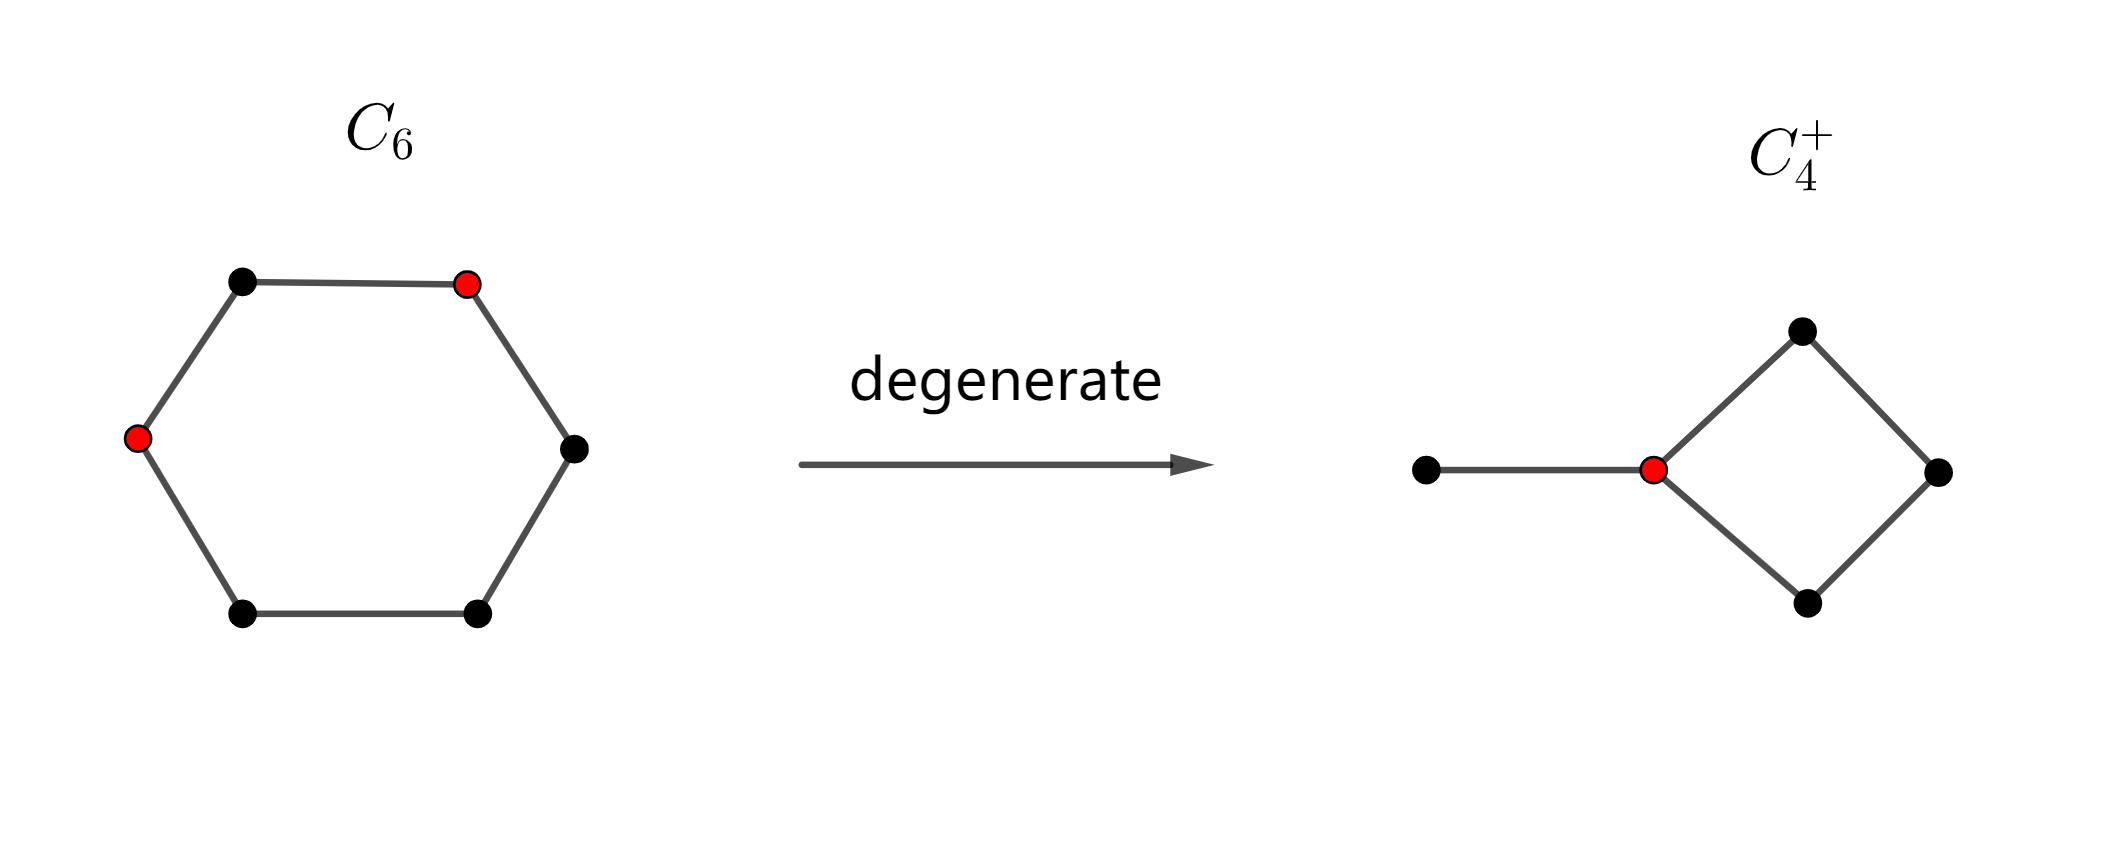
\includegraphics[scale=0.6]{10-1.png}
     \caption{$C_6$ degenerate to $C_4^+$.}
     \label{10-1}
\end{figure}
\begin{proof}
By regularization lemma, we may assume our graph $G$ is $K$-almost-regular. Let $G$ be a $n$-vertex graph with $\Delta(G)\leq K\delta(G)$ and $e(G)\geq Cn^{4/3}$, where $K\ll C$. Write $p=\frac{2e(G)}{n^2}\geq \frac{2C}{n^{2/3}}$.

The Sidorenko's Conjecture implies that $hom(C_6,G)\geq n^6 p^6$. Suppose all of those $C_6$-homomorphisms are degenerate. Since every degenerate $C_6$-homomorphism is a homomorphism of $H:=C_4^+$, so we have $$hom(C_4,G)\cdot \Delta(G)\geq hom(H,G)=hom(C_6,G)\geq n^6p^6.$$ 
It implies that $hom(C_4,G)\geq \frac{n^6p^6}{Knp}=n^5p^5/K$. Then $G$ contains at least $\frac{1}{2K}n^5p^5$ copies of $G$. Indeed, every degenerate $C_4$-homomorphism is a homomorphism of $P_3$, we have 
$$hom(P_3,G)\leq n\Delta(G)^2= K^2n^3p^2 \ll \frac{1}{K}n^5p^5\leq  hom(C_4,G).$$

Now we build an auxiliary graph $\Gamma$ of $G$ with $V(\Gamma)=E(G)$, where $e$ is adjacent to $e'$ in $\Gamma$ if $e\cup e'$ contains a $C_4$ in $G$. Note that if there is a $P_3$ in $\Gamma$, then $G$ contains a $C_6$. We say a $P_3=\{e,f,g\}\subseteq \Gamma$ is $nice$ if $V(e)\cap V(g)=\varnothing$ in $G$, and $bad$ otherwise.

\begin{figure}[h]
     \centering
     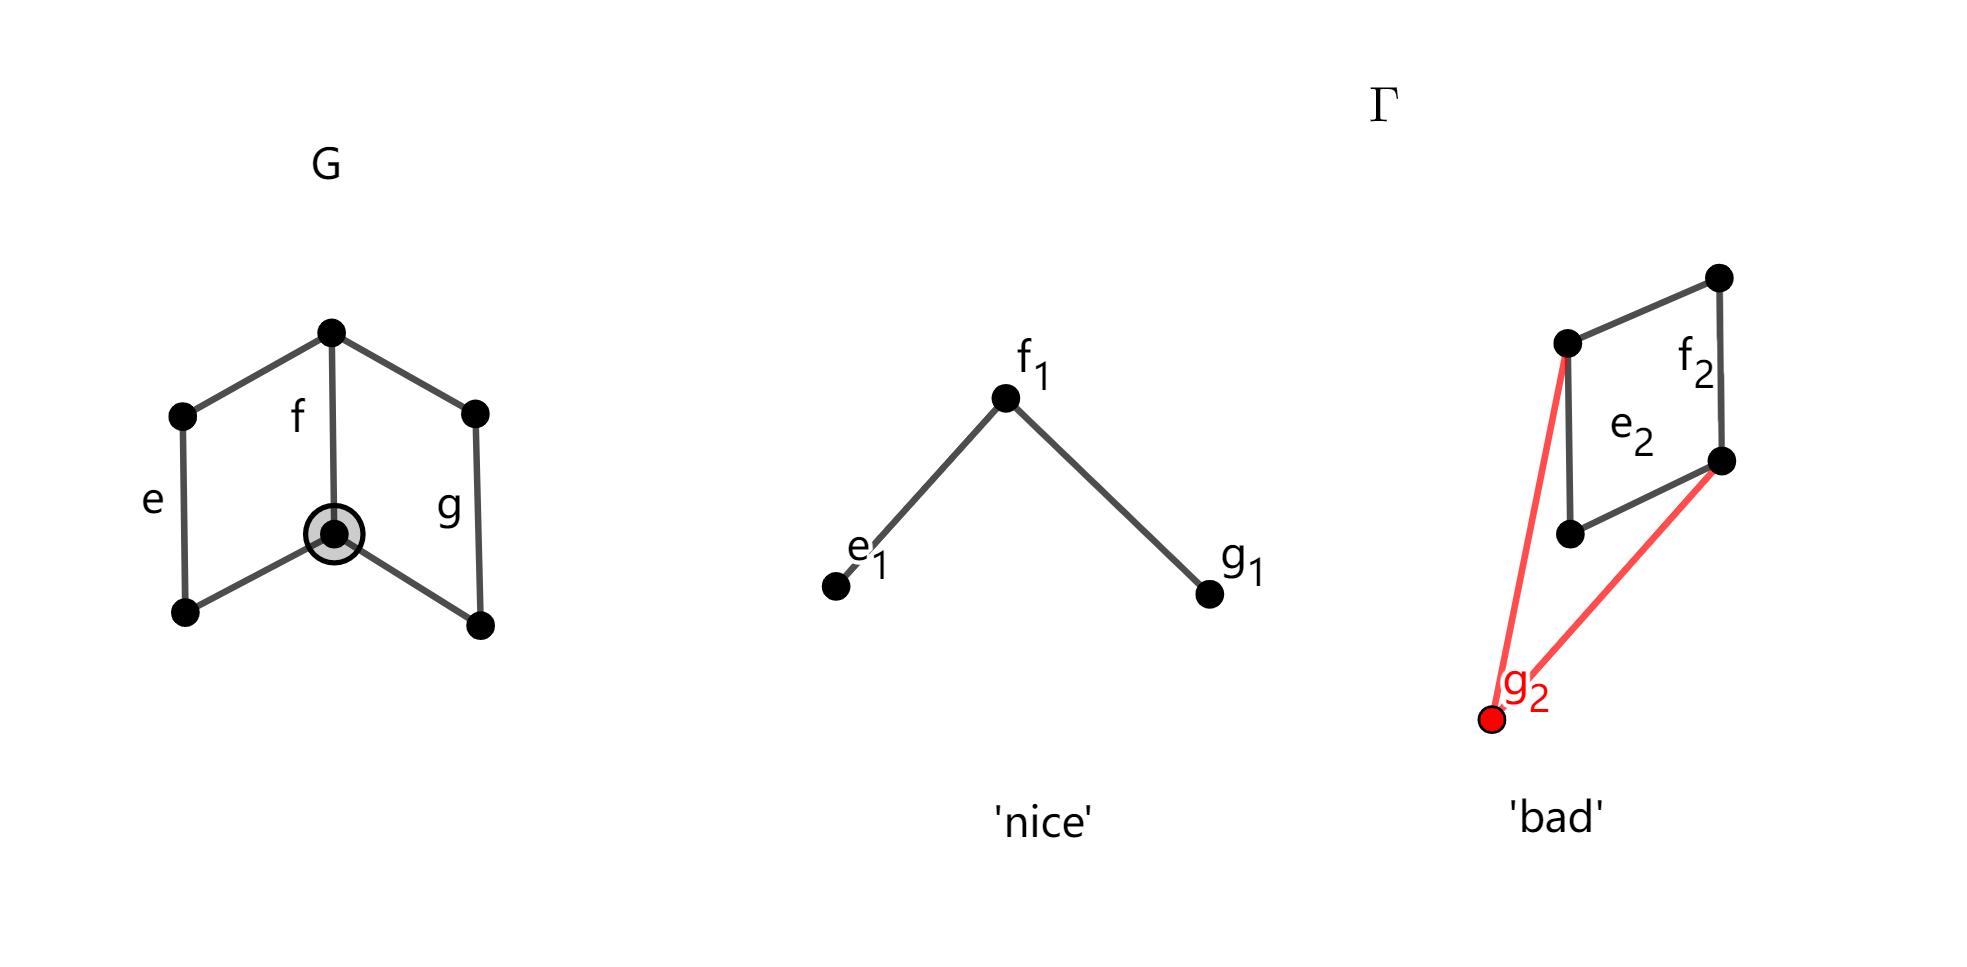
\includegraphics[scale=0.6]{10-2.png}
     \caption{‘nice’ $P_3$ and ‘bad’ $P_3$.}
     \label{10-1}
\end{figure}

Let $m$ be the number of $C_4$ in $G$. Since the average degree of $\Gamma$ is at least $\frac{m}{e(G)}\geq \frac{n^5p^5/2K}{n^2p/2}=n^3p^4/K$, there exists a graph $\Gamma'\subseteq \Gamma$ with $\delta(\Gamma')\geq d(\Gamma)/2$. Pick arbitrary $e\in V(\Gamma)$ and $f\in N_{\Gamma'}(e)$, as the number of bad choices of $g$ is at most $2\Delta(G)\ll d_{\Gamma'}(f)$, there is a nice $P_3$ in $\Gamma'$, which completes the proof.
\end{proof}

\begin{exercise}
    Prove ${\rm ex}(n,C_{2k})=O(n^{1+\frac{1}{k}})$ using above idea.
\end{exercise}

\subsection{Supersaturation for 4-cycle}

\begin{proposition}
    For every $n$-vertex graph $G$ with large $n$, $d(G)\geq 2\sqrt{n}$, there exist at least $\frac{d(G)^4}{8}$ copies of $C_4$ in $G$.
\end{proposition}

\begin{proof}
Let $d=d(G)$. Denote $C$ by the number of cherries $K_{1,2}$ in $G$, we have $$C\geq \sum_{v\in V(G)} \binom{d(v)}{2} \geq n        \binom{\frac{1}{n}\sum d(v)}{2} =n \binom{d}{2},$$ where the first inequality holds by Jensen's inequality. Denote $D$ by the average co-degree of a pair of vertices in $G$, we have
$$ D =\frac{1}{\binom{n}{2}} \sum_{u,v\in \binom{V(G)}{2}}d(u,v) =\frac{C}{\binom{n}{2}} \geq \frac{n\binom{d}{2}}{\binom{n}{2}} \geq \frac{d(d-1)}{n-1} \geq 2.
$$
So the number of $C_4$ in $G$ is at least $$ \sum_{u,v\in \binom{V(G)}{2}}\binom{d(u,v)}{2} \geq \binom{n}{2} \binom{D}{2} \geq \frac{d^4}{8},$$
where the first inequality holds by Jensen's inequality.
\end{proof}


\newpage

\section{Lecture 11: Applications of Sidorenko's Conjecture and Supersaturations}

\subsection{3-dimensional Cube $Q_{3}$}

A 3-dimensional cube is the graph shown in the figure:

\begin{figure}[h]
     \centering
     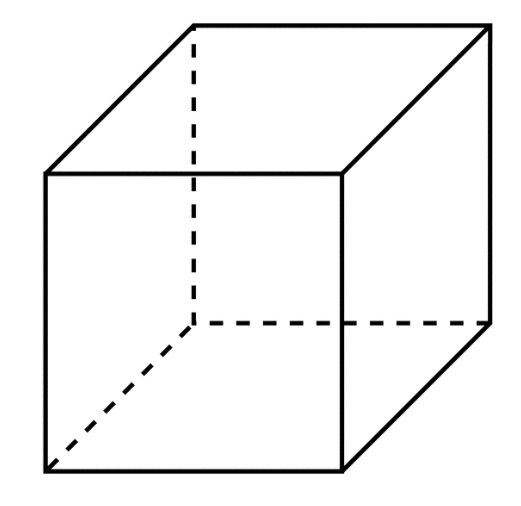
\includegraphics[scale=0.6]{11-1.png}
\end{figure}

Recall that KST theorem~\cite{kHovari1954problem} states $\ex(n,K_{r,t})=O(n^{2-1/r})$, where $r\leq t$. Since $Q_{3}\subseteq K_{4,4}$, we have $\ex(n,Q_{3})\leq cn^{2-1/4}=cn^{7/4}$ for some constant $c=c(n)$. FAKS Theorem~\cite{Furedi1991,Alon2003} states that a bipartite graph with bipartition $A\cup B$ where each vertex in $A$ has degree at most $r$ in $B$, then $\ex(n,H)=O(n^{2-1/r})$. We have $\ex(n,Q_{3})\leq cn^{2-1/3}=cn^{5/3}$ for someconstant $c=c(n)$. Notice that although $Q_{3}$ is 3-regular, it does not contain $K_{3,3}$ as a subgraph, so it seems the upper bound can be improved. In this part, we will give a better upper bound of $\ex(n,Q_{3})$:

\begin{theorem}
    $\ex(n,Q_{3})\leq\ex(n,Q_{3}^{+})=O(n^{8/5})$, where $Q_{3}^{+}$ is $Q_{3}$ unions one longest diagonal.
\end{theorem}

\begin{remark}
    For the lower bound, we only have $\ex(n,Q_{3}^{+})=\Omega(n^{3/2})$, this bound is from the \Turan{} number of $C_{4}$.
\end{remark}

The proof idea is considering supersaturation for $C_{4}$, and there exists one edge $e=xy$ sitting in many 4-cycles. Then we can find 6-cycle in $G[N(x),N(y)]$, and a $Q_{3}^{+}$ is found.

\begin{proof}
    We need to show for any $n$-vertex graph $G$ with $C\cdot n^{8/5}$ edges, we can find $Q_{3}$ in $G$. Recall the supersaturation for $C_{4}$: any n-vertex graph with $d(G)\geq 2\sqrt{n}$, then there are at least $d(G)^{4}/8$ copies of $C_{4}$ in $G$. By regularization trick of Erd\"os-Simonovits, we can assume $G$ is $K$-regular:
    $$Cn^{3/5}\leq \delta(G)\leq \Delta(G)\leq K\delta(G)\leq KCn^{3/5}.$$

    By supersaturation of $C_{4}$, the number of $C_{4}$ in $G$ is at least $\frac{d(G)^{4}}{8}$. By averaging, there exists one edge $e=xy$ lying in at least $\frac{\# C_{4}}{e(G)}\geq \frac{d(G)^{4}/8}{nd(G)/2}=\frac{d(G)^{3}}{4n}\geq \frac{C^{3}n^{4/5}}{4}$ many 4-cycles. Each such $C_{4}$ gives an edge in $G'=G[N(x),N(y)]$. So $e(G')\geq \frac{C^{3}n^{4/5}}{4}$. The number of vertices of $G'$ is at most $2\Delta(G)\leq 2KCn^{3/5}\coloneqq N$ because $x$ and $y$ have at most such many neighbors. To find a $C_{6}$ in $G'$, by Bondy-Simonovits Theorem~\cite{bondy1974cycles}(Theorem~\ref{bstc}) on \Turan{} number of $C_{6}$, we only need $\frac{C^{3}n^{4/5}}{4}>10N^{4/3}$, which is easy to satisfy when $C\gg K$.
\end{proof}

\subsection{Grid $G_{t,t}$}

$G_{t,t}$ is a $t\times t$ grid, as shown in the following figure:

\begin{figure}[H]
     \centering
     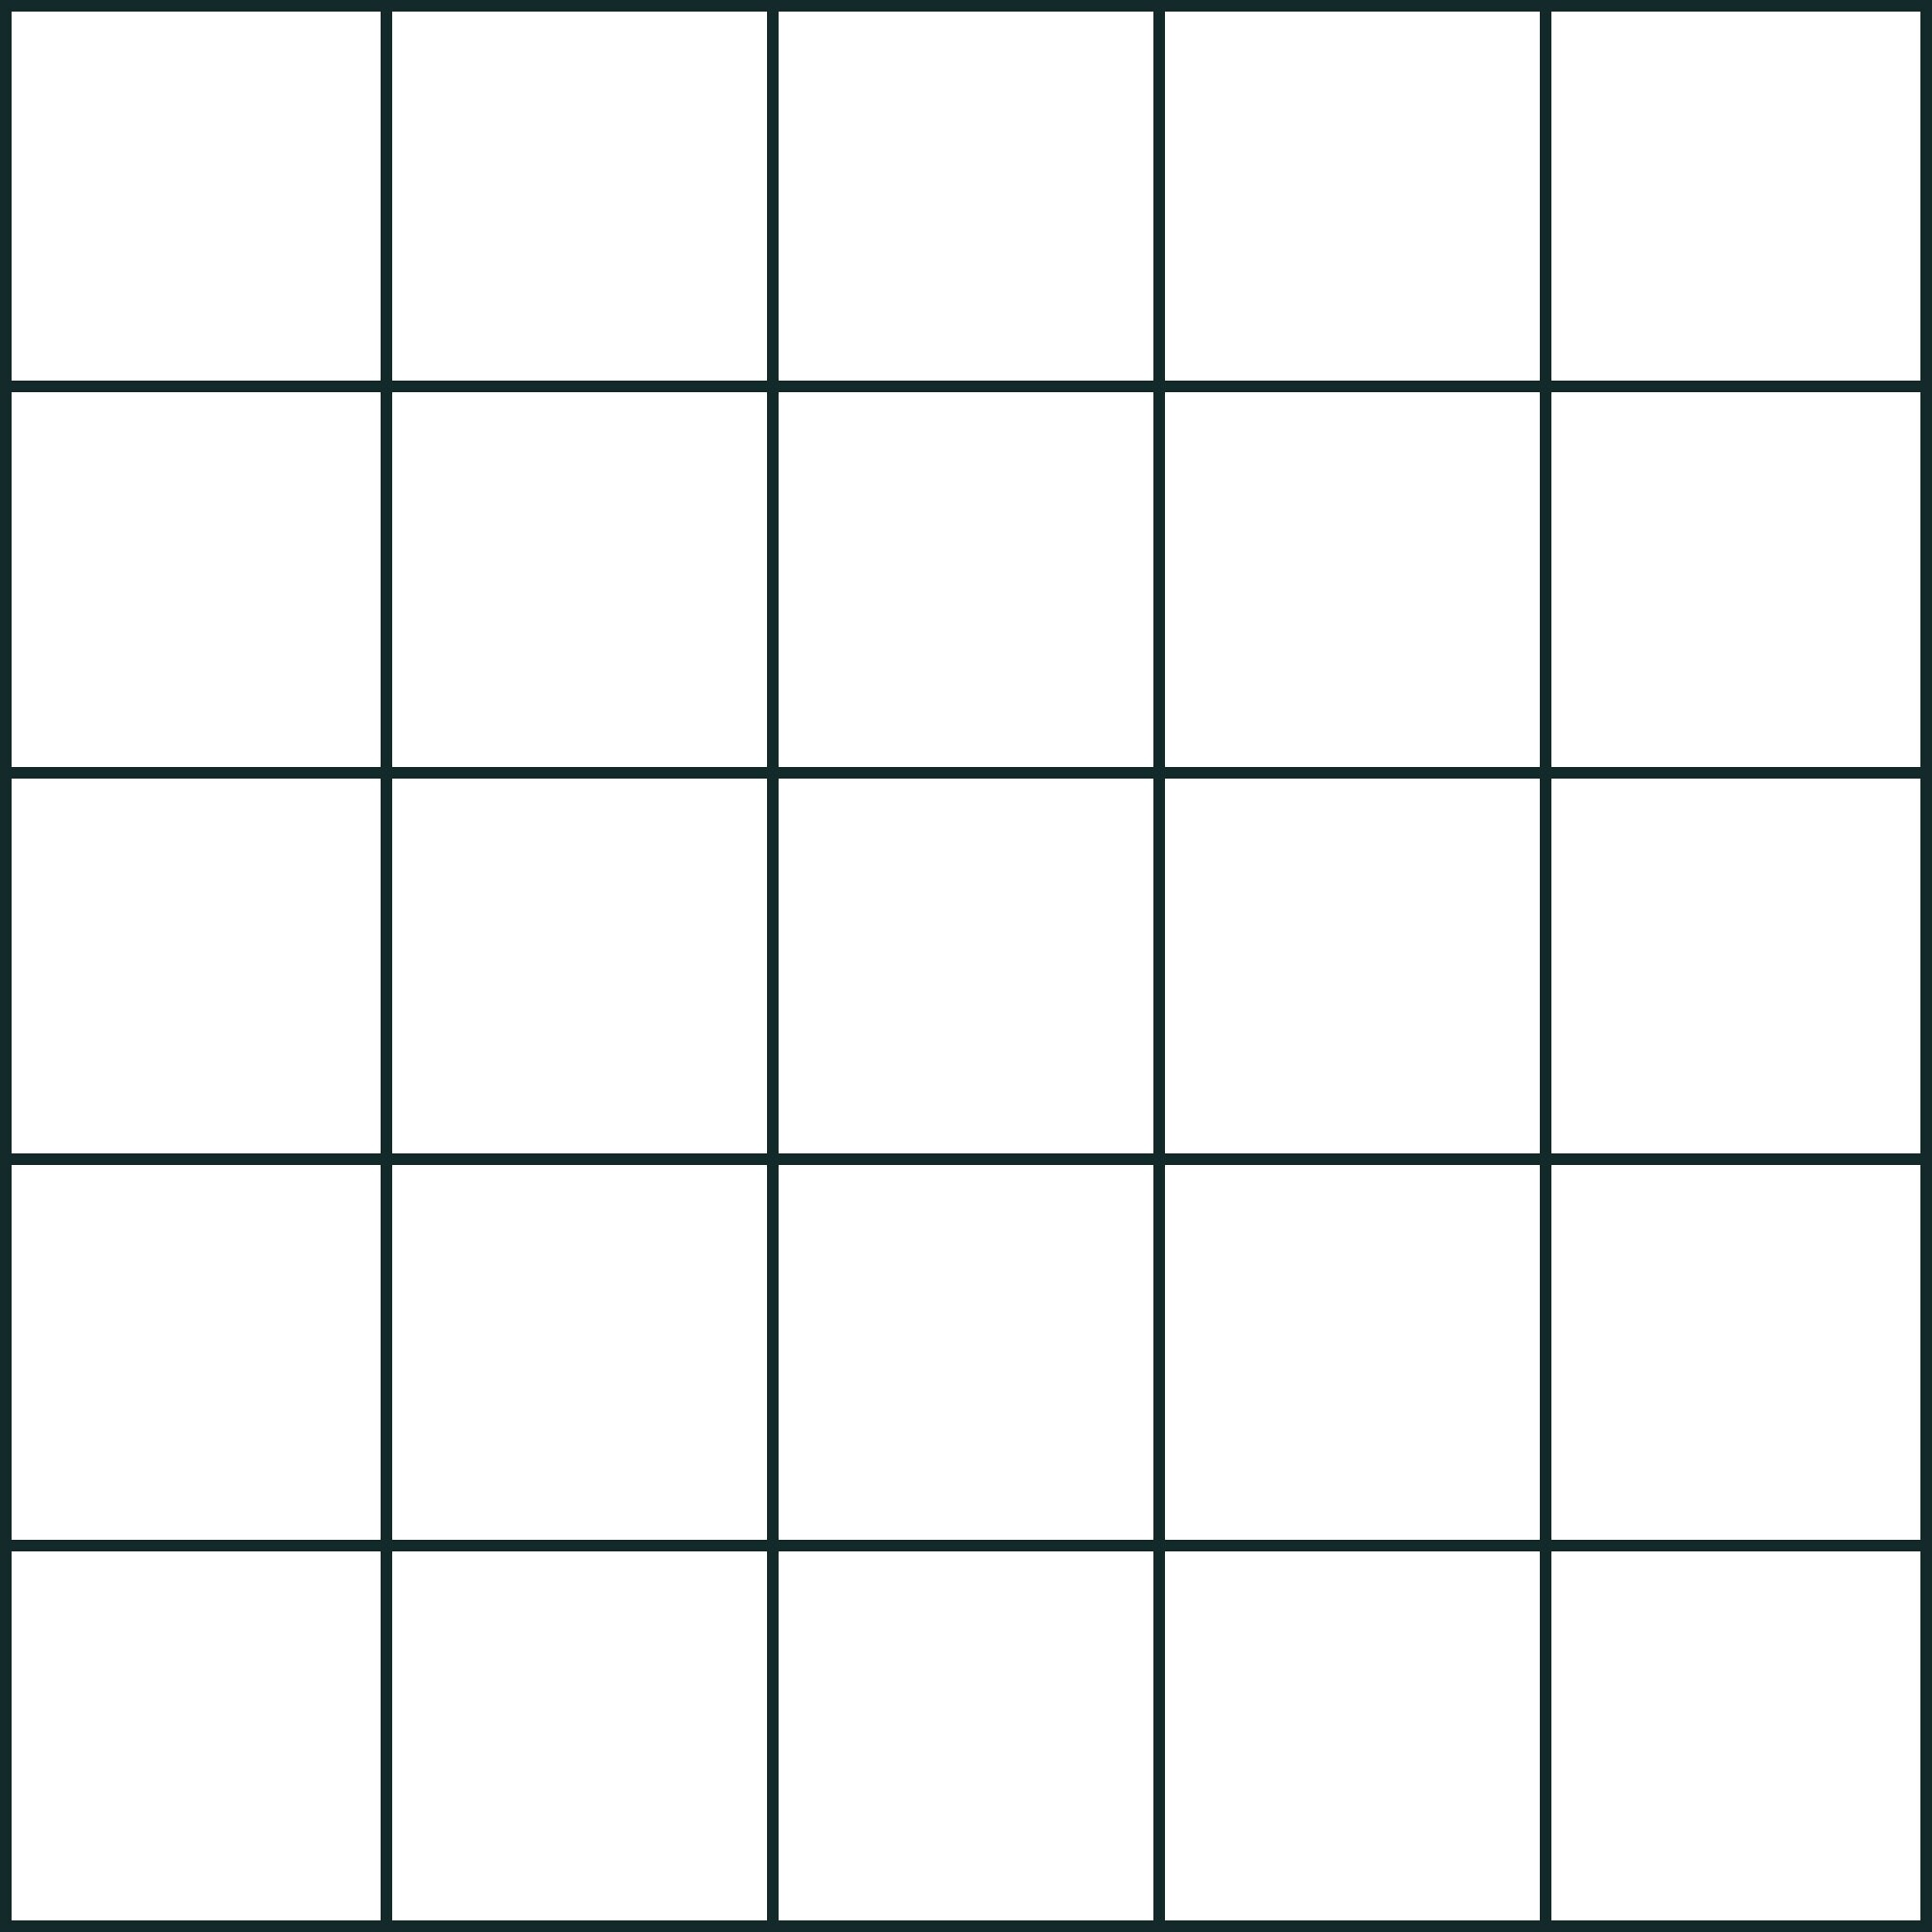
\includegraphics[scale=0.05]{11-2.png}
\end{figure}

Since $C_{4}\subseteq G_{t,t}$, we have $\ex(n,G_{t,t})\geq \ex(n,C_{4})=\Omega(n^{3/2})$. And the upper bound of $\ex(n,G_{t,t})$ is also $O(n^{3/2})$. The first proof was given by Brada\v{c}-Janzer-Sudakov-Tomon~\cite{bradavc2023turan} fairly recently:

\begin{theorem}~\cite{bradavc2023turan}
    $\Omega(t^{1/2}n^{3/2})\leq \ex(G_{t,t})\leq e^{O(t^{5})n^{3/2}}$.
\end{theorem}

Their proof is not long but involves using some initial weaker bound and use tensor power trick to bootstrap the bound to the tight one. Gao-Janzer-Liu-Xu~\cite{gao2023extremal} gave another proof using supersaturation and homomorphism inequality, which is much shorter and can get a better upper bound:

\begin{theorem}~\cite{gao2023extremal}
    $\ex(n,G_{t,t})\leq 5t^{3/2}n^{3/2}$.
\end{theorem}

\begin{remark}
    It would be interesting to determine leading constant $5t^{3/2}$.
\end{remark}

The proof utilizes a strategy that reduces the embedding problem to finding a collection of paths with a certain nice property. So we begin with a definition for a certain collection of paths:

\begin{definition}($\alpha$-rich)
    Let $\alpha>0$ and $k\in\mathbb{N}$. We say that a collection $\mathcal{P}$ of (labelled) paths $P_{k}$ is \emph{$\alpha$-rich} if for any member $x_1x_2\cdots x_k\in\mathcal{P}$ and any $2\leq i\leq k-1$, there exist at least $\alpha$ distinct vertices $x_i'$ such that $x_1x_2\cdots x_{i-1}x_i'x_{i+1}\cdots x_k\in \mathcal{P}$.
\end{definition}

\begin{proposition} (Finding a grid from a rich collection of paths)
    Let $\mathcal{P}$ be a non-empty $\alpha$-rich collection of paths of length $2t-2$ in $G$.
    If $\alpha \ge  t^2$, then $G$ contains a copy of $G_{t,t}$ as a subgraph. 
\end{proposition}

\begin{proof}
    Let $Q_0=x_{1,1}x_{1,2}\cdots x_{1,t}x_{2,t}\cdots x_{t,t}$ be a path in $\mathcal{P}$. Since $\mathcal{P}$ is $\alpha$-rich, we can replace $x_{1,t}$ by a different vertex $x_{2,{t-1}}$ and get another path $Q_1=x_{1,1}x_{1,2}\cdots x_{1,t-1}x_{2,t-1}x_{2,t}x_{3,t}\cdots x_{t,t}$ in $\mathcal{P}$. Again, since $\mathcal{P}$ is $\alpha$-rich and $Q_1\in \mathcal{P}$, we can replace $x_{1,t-1}$ by a vertex $x_{2,t-2}$ that is different from all the previous vertices and get another path $Q_2=x_{1,1}x_{1,2}\cdots x_{1,t-2}x_{2,t-2}x_{2,t-1}x_{2,t}x_{3,t}\cdots x_{t,t}$ in $\mathcal{P}$. We may continue like this and eventually get a path $Q_{t-1}=x_{1,1}x_{2,1}x_{2,2}\cdots x_{2,t}x_{3,t}\cdots x_{t,t}$ in $\mathcal{P}$. Then we may replace $x_{2,t}$ by a vertex $x_{3,t-1}$ that is different from all previous vertices, and get a path $Q_t=x_{1,1}x_{2,1}x_{2,2}x_{2,3}\cdots x_{2,t-1}x_{3,t-1}x_{3,t}x_{4,t}\cdots x_{t,t}$ in $\mathcal{P}$. Continuing this process in the obvious way, we end up with a path $x_{1,1}x_{2,1}\cdots x_{t,1}x_{t,2}\cdots x_{t,t}$ in $\mathcal{P}$. The vertices $x_{i,j}$ ($i,j\in [t]$) defined through this process form a $t\times t$ grid (e.g. for $t=4$, see the following figure).
\end{proof}

\begin{figure}[H]
     \centering
     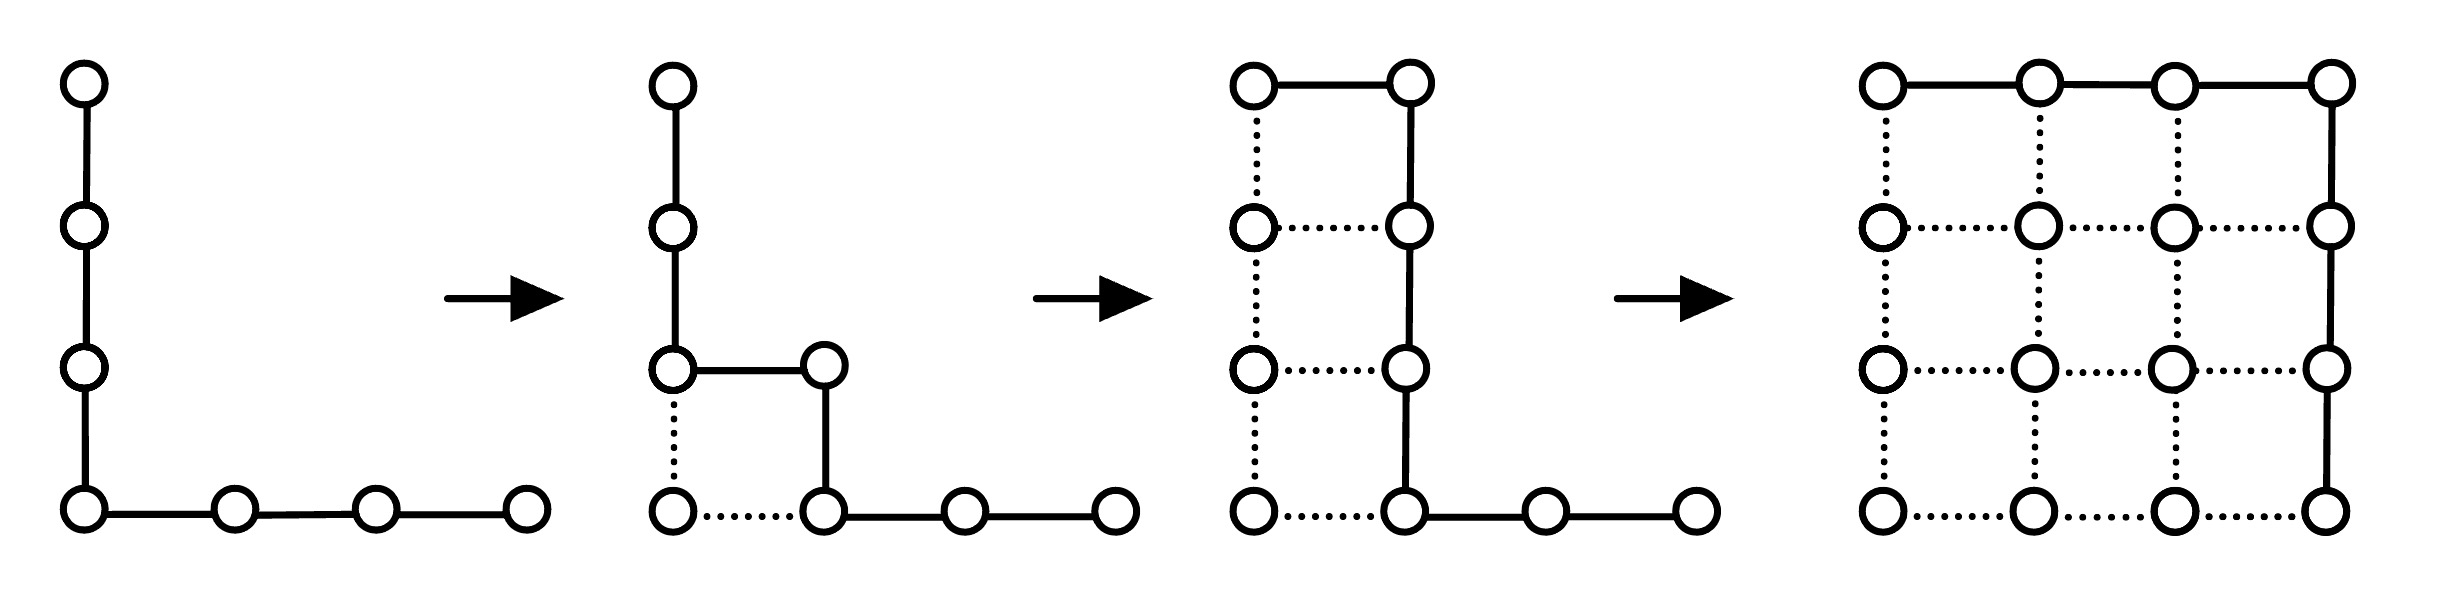
\includegraphics[scale=0.15]{11-3.png}
\end{figure}

\begin{lemma}
    Let $t$ be a positive integer, let $n$ be sufficiently large compared to $t$ and let $G$ be an $n$-vertex graph with  $e(G)\geq 5t^{3/2}n^{3/2}$. Then $G$ has a non-empty $\alpha$-rich collection of paths of length $2t-2$ with $\alpha=t^2$.
\end{lemma}

\begin{proof}
    We may assume $G$ is $K$-almost regular by regularization trick and $d(G)\geq 10t^{3/2}n^{1/2}$. Let $\alpha=t^2$. Let $\mathcal{P}_0$ be the collection of paths of length $2t-2$ in $G$. Since $G$ is $K$-almost regular, it is easy to see that more than half of all homomorphisms from $P_{2t-1}$ to $G$ are injective. Hence, we have $|\mathcal{P}_0|\geq \frac{1}{2}\hom(P_{2t-1},G)$.
    
    Define a sequence of collections of paths of length $2t-2$ in $G$, $\mathcal{P}_0 \supseteq \mathcal{P}_1 \supseteq \cdots$. Having defined $\mathcal{P}_i$, if there exist some $P\in \mathcal{P}_i$ and an internal vertex $a\in P$ such that the number of $P'\in \mathcal{P}_i$ containing some $b\in P'$ with $P'-b = P-a$ is less than $\alpha$, then define $F_{i}:=P-a$ and let $\mathcal{P}_{i+1}$ be the collection obtained from $\mathcal{P}_i$ by removing all paths of length $2t-2$ containing $F_{i}$. The process will terminate if there is no such member $P$.

    Suppose that the process stops after $s$ steps, it suffices to show that $\mathcal{P}_{s}$ is non-empty. As for each $i\in \{0,1,\ldots,s-1\}$, all paths of length $2t-2$ in $\mathcal{P}_{i}$ containing $F_{i}$ were removed, all the $F_{i}$'s are distinct. Hence the number of possible steps $s$ is at most the number of different possibilities for $F_i$.

    \begin{claim}
        There are at most $\frac{1}{4t^2}\hom(P_{2t-1},G)$ possibilities for $F_i$.
    \end{claim}

    Before we prove the claim, we need the following lemma by Erd\"os and Simonovits~\cite{erdHos1982compactness}:

    \begin{lemma}~\cite{erdHos1982compactness}\label{erdHos1982compactness}
        Let $k>\ell$ be positive integers such that $k$ is even. Then for any $n$-vertex graph $G$, we have
        $(\frac{\hom(P_{k+1},G)}{n})^{1/k}\geq (\frac{\hom(P_{\ell+1},G)}{n})^{1/\ell}$.
    \end{lemma}


\begin{poc}
 There are less than $2t$ choices for the position of the removed vertex, so it suffices to prove that for each $0\leq \ell\leq 2t-4$, the number of subgraphs in $G'$ isomorphic to $P_{\ell+1}\cup P_{2t-3-\ell}$ is at most $\frac{1}{8t^3}\hom(P_{2t-1},G)$. Clearly, the number of such subgraphs in $G'$ is at most $\hom(P_{\ell+1},G)\hom(P_{2t-3-\ell},G)$. By Lemma \ref{erdHos1982compactness}, we have
    \begin{align*}
        \hom(P_{\ell+1},G)\hom(P_{2t-3-\ell},G)
        &\leq m\left(\frac{\hom(P_{2t-1},G)}{m}\right)^{\ell/(2t-2)}m\left(\frac{\hom(P_{2t-1},G)}{m}\right)^{(2t-4-\ell)/(2t-2)} \\
        &=m^2\left(\frac{\hom(P_{2t-1},G)}{m}\right)^{(2t-4)/(2t-2)} \\
        &=m^{\frac{t}{t-1}}\hom(P_{2t-1},G)^{(t-2)/(t-1)}.
    \end{align*}
    By Sidorenko's property for paths, we have $\hom(P_{2t-1},G)\geq md^{2t-2}$, so $\hom(P_{2t-1},G)^{1/(t-1)}\geq m^{1/(t-1)}d^2\geq 16t^3m^{t/(t-1)}$. Hence, $m^{\frac{t}{t-1}}\hom(P_{2t-1},G)^{(t-2)/(t-1)}\leq \frac{1}{16t^3}\hom(P_{2t-1},G)$, completing the proof of the claim.   
\end{poc}
    By the claim and our earlier discussion, it follows that $s\leq \frac{1}{4t^2}\hom(P_{2t-1},G)$.
    Hence, we have 
    \begin{equation*}
        |\mathcal{P}_{s}| \ge |\mathcal{P}_0|-s\cdot \alpha \ge  \frac{1}{2}\hom(P_{2t-1},G)-  st^2 >0,
    \end{equation*}
     as desired.
\end{proof}

\subsection{The Third Proof of \Turan{} number for $C_{2k}$}

In this part, we will give the third proof of Bondy-Simonovits theorem: $\ex(n,C_{2k})=O(n^{1+1/k})$, using Sidorenko's conjecture and iterative Cauchy-Schwarz inequality. This is indepedently discovered by two groups of people, one is Janzer-Sudakov~\cite{janzer2024turan} and another is Kim-Lee-Liu-Tran~\cite{kim2022rainbow}.

The idea is: we may first assume $G$ is $K$-regular with $n$ vertices and at least $Cn^{1+1/k}$ edges. If most of $C_{2k}$-homomorphism are non-degenerate, then we are done. So most of $C_{2k}$-homomorphism are degenerate. We can show that positive fraction of $C_{2k}$-homomorphism are homomorphism of $C_{2k-2}^{+}$, where $C_{2k-2}^{+}$ is $C_{2k}$ unions one pendent edge. And the number of homomorphism of $C_{2k-2}^{+}$ is almost the same as the number of homomorphism of $C_{2k-2}$. Now we use Cauchy-Schwarz iteratively to prove that the number of homomorphism of $C_{2k}$ is almost the same as the number of homomorphism of the star $S_{k}$. Then we have:
$$n^{k+1}p^{k}\geq n\Delta(G)^{k}\geq\hom(S_{k},G)\approx\hom(C_{2k},G)\geq n^{2k}p^{2k},$$
where the first inequality follows from the $K$-almost regular property, and the last inequality follows from Sidorenko's conjecture. Solving this inequality we get $p\leq n^{1/k-1}$. But $e(G)\geq Cn^{1+1/k}$, a contradiction.

We illustrate it with $C_{8}$, we may assume that $G$ is an $n$-vertex, $K$-almost regular graph with average degree $d\geq Cn^{1/4}$. Then the edge density $p=d/n=Cn^{-3/4}$. There are only two kinds of `largest' degenerate homomorphism:

\begin{itemize}
    \item Identify two vertices with distance 2 in the cycle $C_{8}$ (see the following figure from $G_{1}$ to $T_{1}$).
    \item Identify two vertices with distance 4 in the cycle $C_{8}$ (see the following figure from $G_{2}$ to $T_{2}$).
\end{itemize}

\begin{figure}[H]
     \centering
     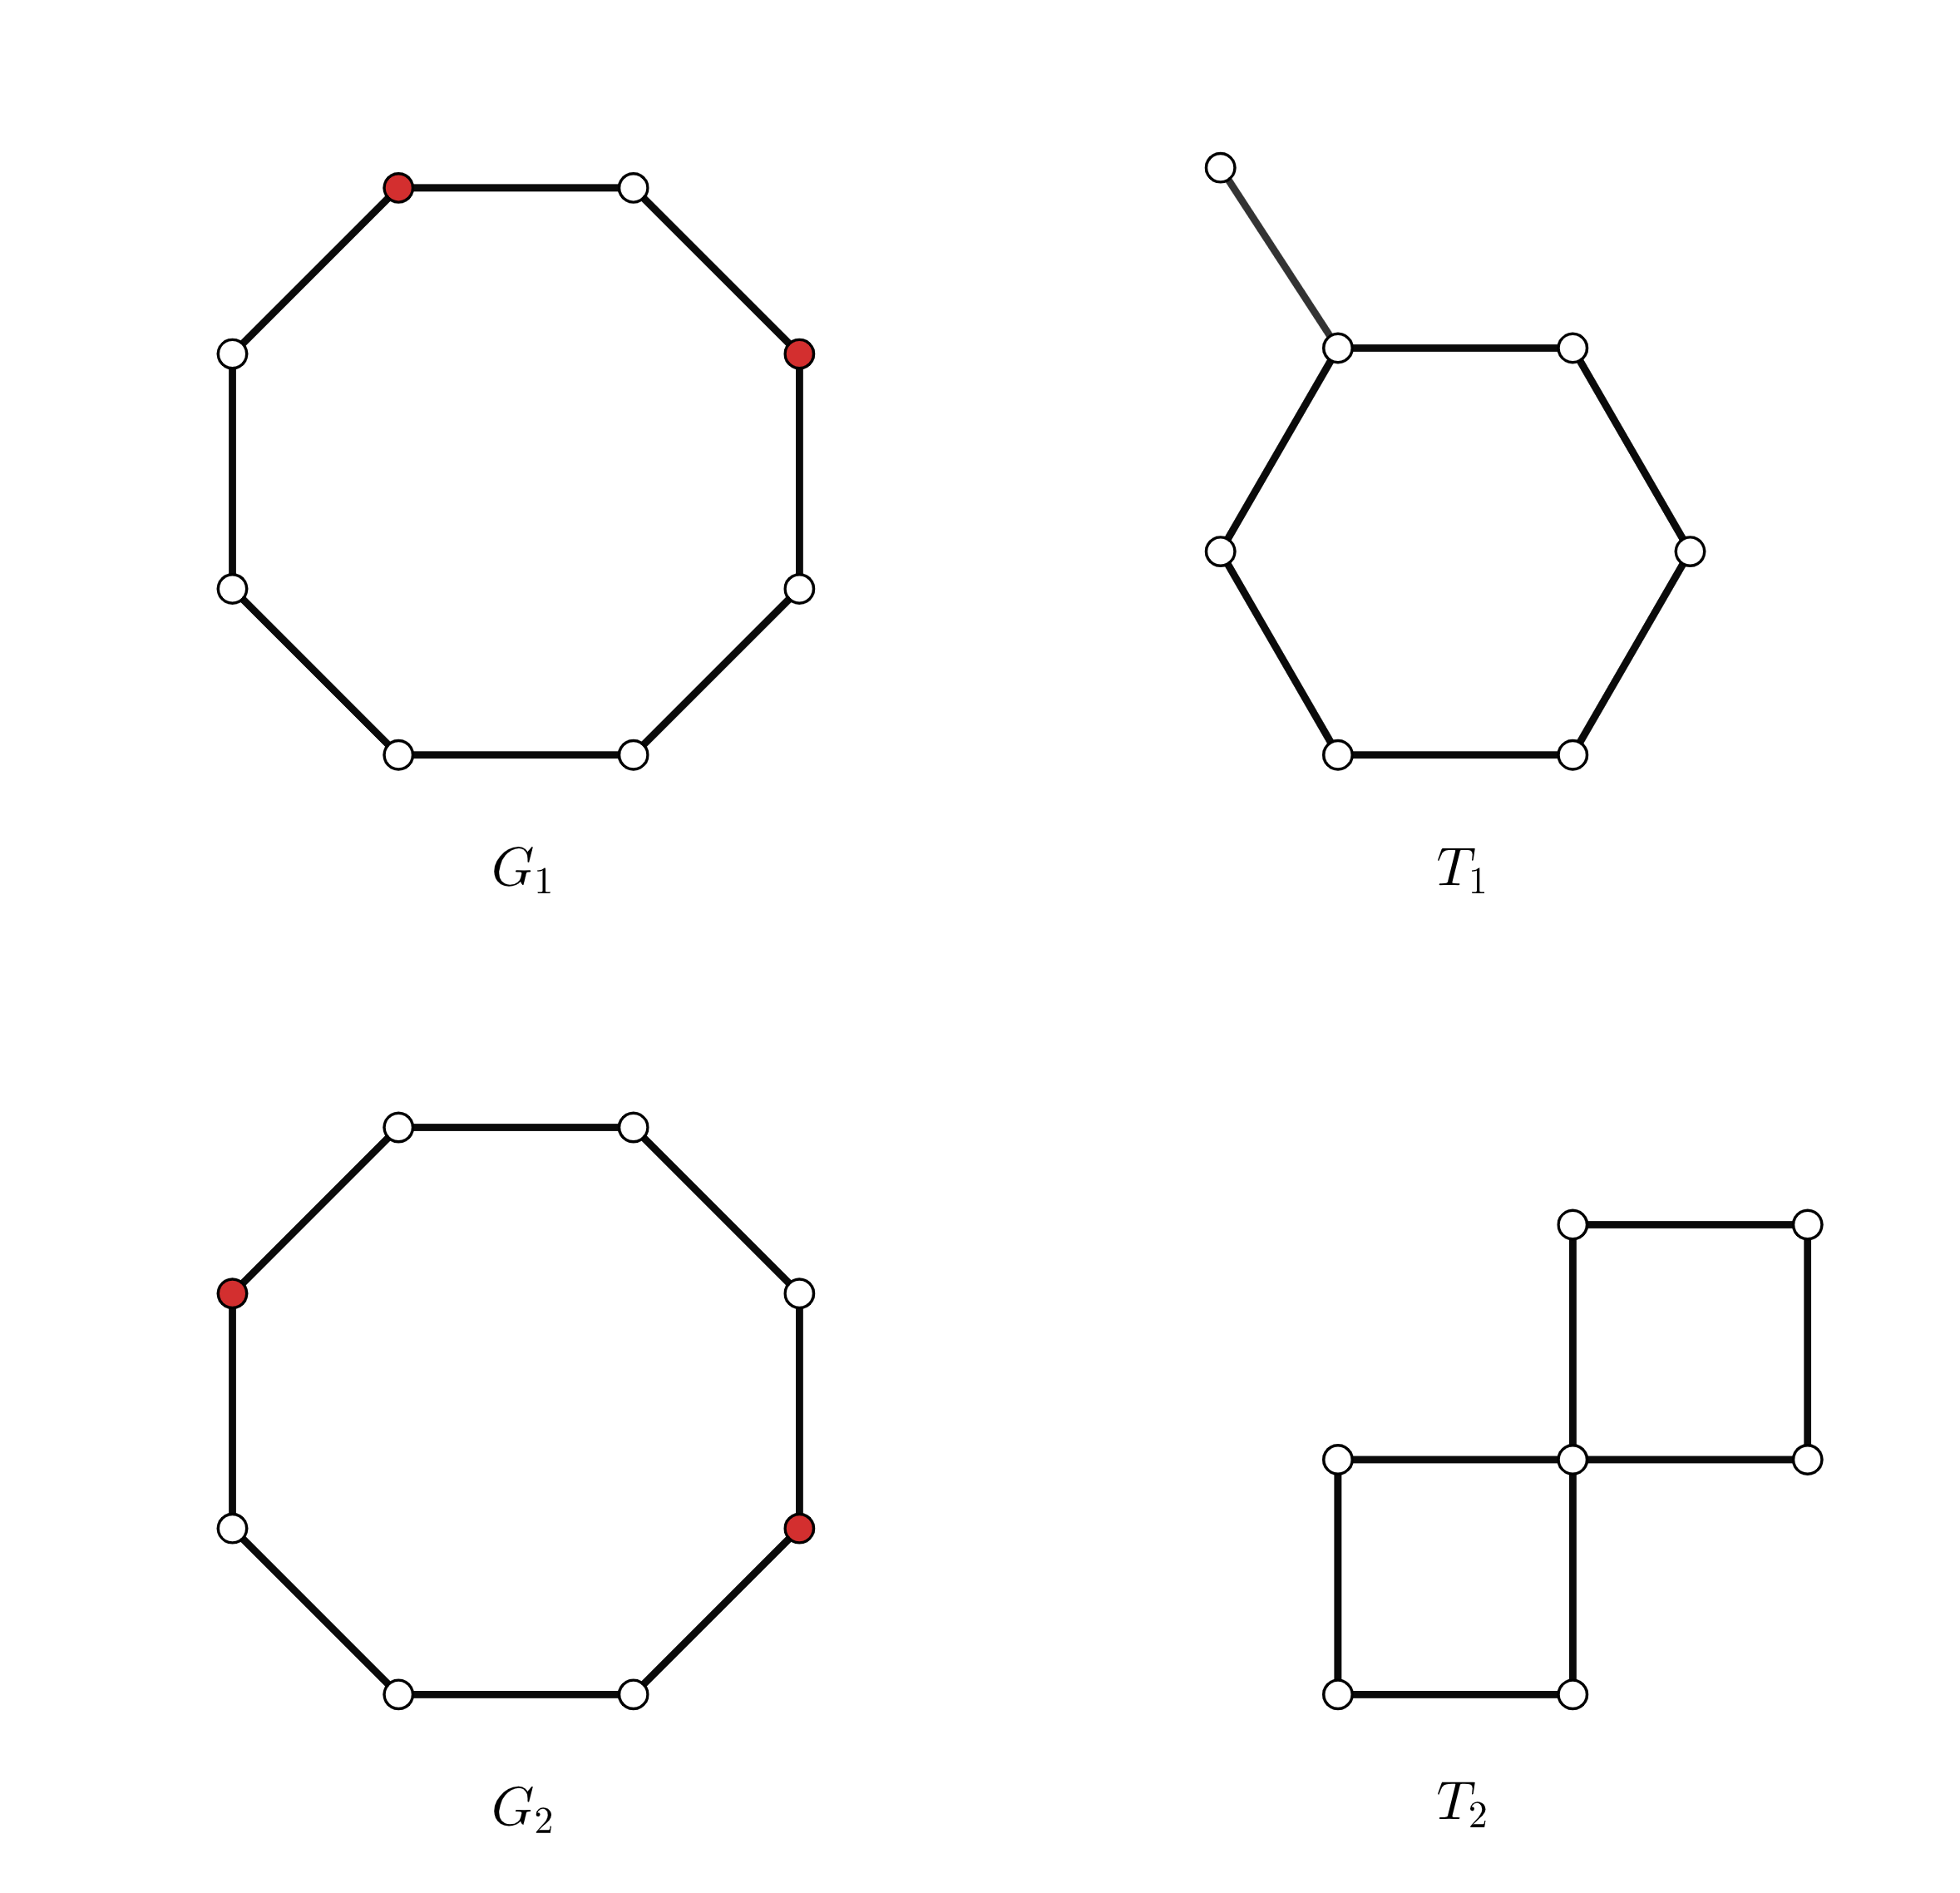
\includegraphics[scale=0.25]{11-4.png}
\end{figure}

Let $u,v,w$ be the vertices in $T_{2}$, as shown in the following figure.

\begin{figure}[H]
     \centering
     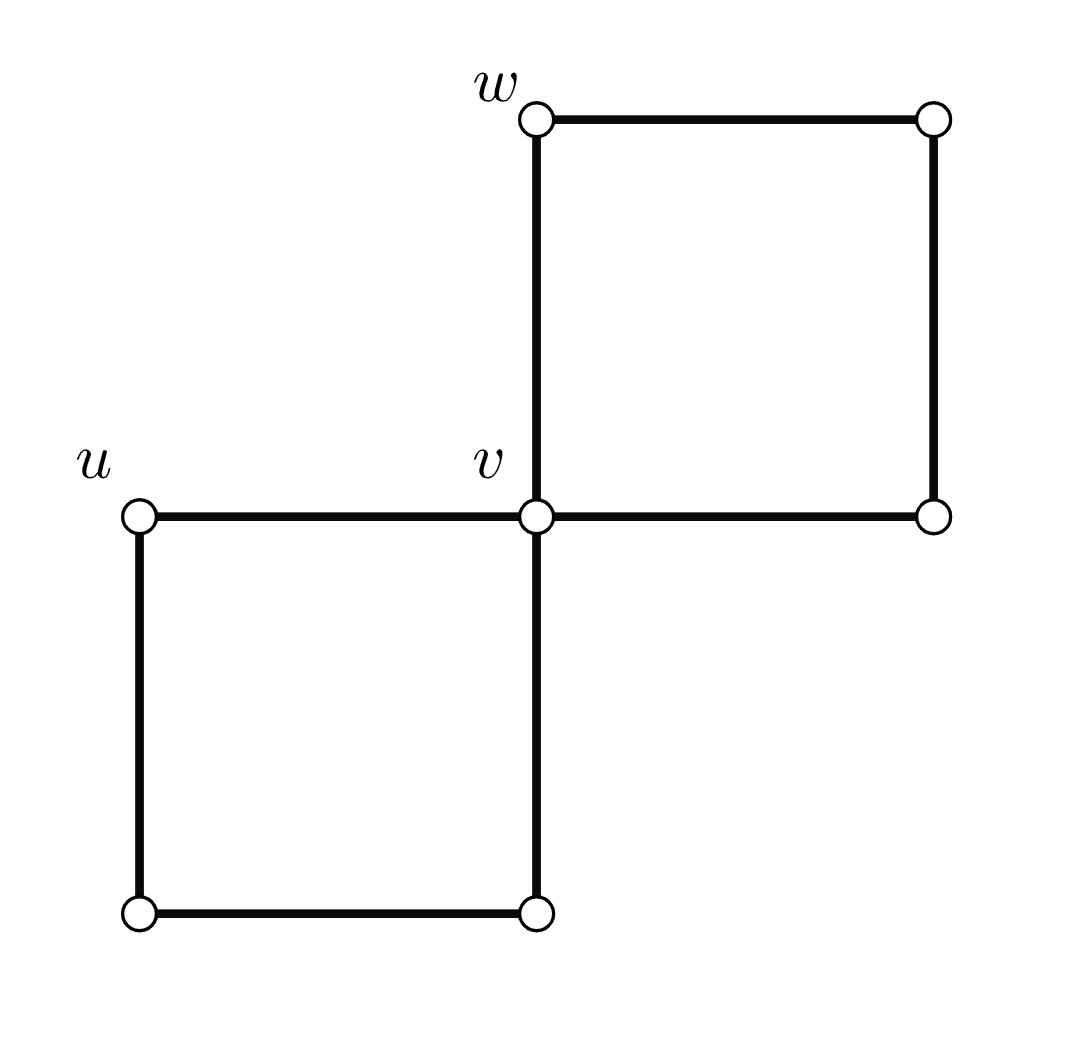
\includegraphics[scale=0.4]{11-5.png}
\end{figure}

Let $\phi$ be a particular $P_{3}$ homomorphism in $G$. Let $a_{\phi}$ be the number of extensions of $\phi$ to $P_{4}$ homomorphism $uxyv$, $b_{\phi}$ be the number of extensions of $\phi$ to $P_{4}$ homomorphism $vqzw$. Then
$$\hom(T_{2},G)^{2}=\sum_{\phi}a_{\phi}b_{\phi}\leq (\sum_{\phi}a_{\phi}^{2})(\sum_{\phi}b_{\phi}^{2})\leq \hom(T_{1},G)^{2}$$
by Cauchy-Schwarz inequality. So we have $\hom(T_{1},G)=\Omega(\hom(C_{2k},G))$. The proof will continue in the next lecture...


\newpage
\section{Lecture 12: Extremal Set Theory--Bollob\'as set-pairs inequality}

Firstly we continue the proof of Lecture 11.

We denote the $C_4$ with two independent edges shared same vertex by $T_3$, denote $P_4$ with identified vertices $u,v$ by $P_{uv1}$, denote $P_5$ with ending vertices vertices $u,v$ by $P_{uv2}$.Then we have that $T_1=P_{uv1}+P_{uv2},T_3=P_{uv1}+P_{uv1}$ and $C_8=P_{uv2}+P_{uv2}$.(see following figure).

\begin{figure}[H]
     \centering
     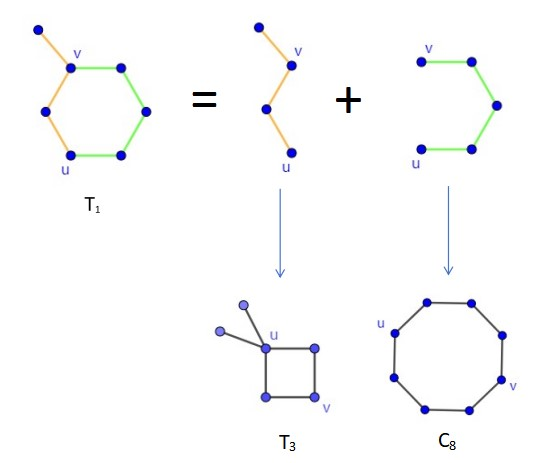
\includegraphics[scale=0.35]{12-1.jpg}
\end{figure}

For the sake of simplicity, we denote $f=\Omega(g)$ by $f\approx g$. We have shown that $hom(T_1,G)\approx hom(C_{2k},G)$, now we are going to show that $hom(T_1,G)^2 \le hom(C_8,G)hom(T_3,G)$.

Let $\varphi$ be $P_3$ with the ending vertices $u,v$ homomorphism in $G$. Let $a_\varphi$ be the number of extension of $\varphi$ to $P_4$ homomorphism $xuyv$, let $b_\varphi$ be the number of extension of $\varphi$ to $P_5$ homomorphism $uxyzv$.Then
$$hom(T_1,G)^2=\sum_{\varphi}a_{\varphi}b_{\varphi}\le (\sum_{\varphi}a_{\varphi}^2)(\sum_{\varphi}b_{\varphi}^2)\le hom(C_8,G)hom(T_3,G)$$ by Cauchy-Schwarz inequality. So we've got that 
$\frac{hom(T_3,G)}{hom(T_1,G)}\le \frac{hom(T_1,G)}{hom(C_8,G)}$.

By a similar discussion, we could get that $\frac{hom(K_{1,4},G)}{hom(T_3,G)}\le \frac{hom(T_3,G)}{hom(T_1,G)}$(see following figure).

\begin{figure}[H]
     \centering
     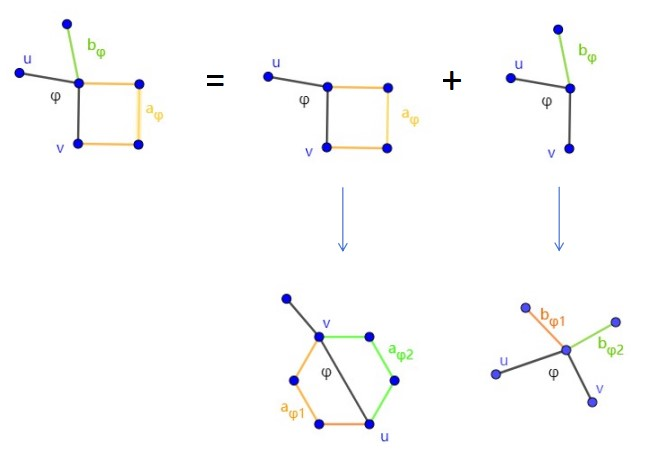
\includegraphics[scale=0.35]{12-2.jpg}
\end{figure}

Now we would show the final contradiction by using Sidorenko's conjecture. Noticed that $$hom(K_{1,4},G)=\frac{hom(K_{1,4},G)}{hom(T_3,G)}\frac{hom(T_3,G)}{hom(T_1,G)}\frac{hom(T_1,G)}{hom(C_8,G)}hom(C_8,G)$$

We've already known that $\frac{hom(T_1,G)}{hom(C_8,G)}=\Omega(1)$. Thus $\frac{hom(K_{1,4},G)}{hom(T_3,G)}\ge \frac{hom(T_3,G)}{hom(T_1,G)}\ge \frac{hom(T_1,G)}{hom(C_8,G)}=\Omega(1)$. In the other hand, $K_{1,4}$ has the most degenerate homomorphism of $C_8$, which means $n^5p^4 \ge hom(T_{1,4},G)$. 

So we have that $$n^5p^4 \ge hom(K_{1,4},G)\ge\Omega(1)hom(C_8,G)\ge n^8p^8$$
which means that $p \le n^{3/4}$. But $e(G)\geq Cn^{1+1/k}$, a contradiction. \qed

\subsection{Rational Exponent Conjecture}

Now we introduce a beautiful conjecture and the work that people have done on it.

\begin{conjecture}(\Turan{} rational exponent conjecture,\Erdos{}\cite{erdosrationalconj},1981)
For any $r \in (1,2)\cup \mathbb{R}$, exists a bipartite graph $H$, such that $ex(n,H)=\Theta(n^r)$.
    
\end{conjecture}

\begin{remark}
    Bukh and Conlon\cite{BukhandConlon} have proved that the conjecture is true if we forbid a finite family of bipartite graphs instead of just one bipartite graph.
\end{remark}

Firstly, we introduce an important techniques.

\begin{definition}[1-subdivision]
    For a graph $G=(V,E)$, its 1-subdivision $Sub(G)$ is a graph whose vertex set $V_1=V\cup E$ and $E_1=\left \{ a\text{ is incident with }b|a\in V,b\in E\right \} $.(see following figure)
\end{definition}

\begin{figure}[H]
     \centering
     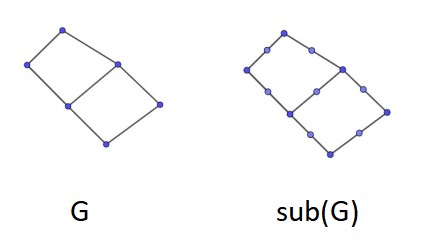
\includegraphics[scale=0.35]{12-3.jpg}
\end{figure}

We propose an approach to tackle the \Turan{} rational exponent conjecture via the following conjecture on subdivision of graphs.

\begin{conjecture}{(1-subdivision conjecture,Kang-Kim-Liu \cite{KANG2021149},2021)}

    Let $F$ be a bipartite graph. If $ex(n,F)=O(1+n^\alpha)$for some $\alpha>0$, then $$ex(n,sub(F))=O(n^{1+\frac{\alpha}{2}})$$
    
\end{conjecture}

\begin{remark}
    If the 1-subdivision conjecture is true, then it implies the \Turan{} rational exponent conjecture.
\end{remark}

\subsection{Bollob\'as set-pair inequality}

Now we start a new part, considering the extremal problem involving sets instead of graphs.

We study the extremal problem for family of sets with various intersection patterns.
We've already seen some examples, such as 
\begin{itemize}
    \item containment $A \subseteq B$ (Sperner)
    \item disjointness $A \cap B = \emptyset$
    \item intersection $A \cap B \neq \emptyset$ (\Erdos{}-Ko-Rado)
\end{itemize}

We also have study some important result in this field, such as 

\begin{itemize}
    \item odd/even town: restriction on parity of size of pairwise intersection
    \item Sperner theorem: the size of the largest antichain in $2^{[n]}$ is $\binom{n}{\lfloor n/2\rfloor}$
    \item LYM-inequality: for any antichain $\mathcal{A} \subseteq 2^{\left [ n \right ] }$,$$\sum_{A\in \mathcal{A}} \frac{1}{\binom{n}{\left | A \right | }} \le 1$$
\end{itemize}

Now we would see some result about the family of sets with restriction on the intersection pattern.
Let's consider a family of pair of sets, and we put restriction in the bipartite faction, more precisely, we put restriction in the cross pairs. 

\begin{theorem}[Bollob\'as set-pair inequality\cite{Bollobassetpair}]
    Given sets $A_1,A_2,\cdots,A_m,B_1,B_2,\cdots,B_m$, if $\left\{\begin{matrix} A_i\cap B_i =\emptyset \quad \forall i\in \left [ m \right ] 
 \\A_i \cap B_j \neq \emptyset \quad \forall i \neq j

\end{matrix}\right.$
then we have $$\sum _{i\in \left [ m \right ] }\frac{1}{\binom{\left | A_i \right |+\left | B_i \right |  }{\left | A_i \right | } } \le 1$$
In particular, if $\forall i \in \left [ m \right ], \left | A_i \right |=a,\left | B_i \right |=b$,then $m \le \binom{a+b}{a}$. 
\end{theorem}

\begin{remark}
    Note that the size of grand set (of $A_i,B_i$) do not play a role.
\end{remark}

\begin{proof}
    Assume ground set is $\left [ n \right ]$. Consider a uniform random permutation $\sigma$ of $\left [ n \right ]$ and label each number $a$ by its position $f(a)$. Let $P_i$ be the event that $A_i$ precedes $B_i$ in $\sigma$, in other words, it means that $\max_{a \in A_i} f(a) \le \min_{b \in B_i} f(b) $. 

    The event $P_i$ only depends on the relative position of $A_i$ and $B_i$. So that $$Pr(P_i)=\frac{\left | A_i \right |!   \left | B_i \right |!  }{\left | A_i \cup B_i \right |! }
=\frac{1}{\binom{\left | A_i \right |+ \left | B_i \right |}{\left | A_i \right |} } $$
    Now we only need to show that $P_i,i\in \left [ m \right ]$ are disjoint events, thus we can get the conclusion $\sum_{i\in \left [ m \right ]}Pr(P_i) \le 1$.

    Suppose that both $P_i$ and $P_j$ occur and $i \neq j$. Noticed that $A_i \cap B_j \neq \emptyset$, so that $\min_{b\in B_j}f(b) \le \max_{a\in A_i}f(a)$. However, $P_i$'s occurs means that $\min_{b\in B_i}f(b) > \max_{a\in A_i}f(a)$, similarly, $\min_{b\in B_j}f(b) > \max_{a\in A_j}f(a)$. Thus we get that $\min_{b\in B_i}f(b) > \max_{a\in A_j}f(a)$, which leads to a contradiction as $A_j \cap B_i \neq \emptyset$.
\end{proof}

\begin{exercise}
    Find an example showing tightness of Bollob\'as set-pair inequality.
\end{exercise}

Now we consider the skewed version of the Bollob\'as set-pair inequality.

\begin{theorem}[Bollob\'as set-pair inequality(skewed version)\cite{2023Bollobasskew}]
    Given sets $A_1,A_2,\cdots,A_m,B_1,B_2,\cdots,B_m$, $\forall i \in \left [ m \right ], \left | A_i \right |\le a,\left | B_i \right |\le b$, if $\left\{\begin{matrix} A_i\cap B_i =\emptyset \quad \forall i\in \left [ m \right ] 
 \\A_i \cap B_j \neq \emptyset \quad \forall i < j
\end{matrix}\right.$
then we have $m \le \binom{a+b}{a}$. 
\end{theorem}

\begin{remark}
    We only have an algebra proof of this skewed version by Lov\'asz, Alon-Kalai\cite{ALON1985211}. Finding a combinational proof would be interesting. 
\end{remark}

We briefly introduce the exterior algebra first. Let $V$ be a vector space over a field $K$, we introduce an operation exterior power.

\begin{definition}[exterior power]
    The $k$-th exterior power of $V$, denoted by $\wedge^k V$, is a vector space spawned by elements of the form $x_1 \wedge x_2 \wedge \cdots \wedge x_k,x_i \in V,\forall i \in \left [ k \right ]$, such that $x_1 \wedge x_2 \wedge \cdots \wedge x_k=0$ if $x_i=x_j$ for some distinct $i,j\in \left [ k \right ]$.
\end{definition}

\begin{example}
    If $\left \{ e_1,e_2,\cdots ,e_n \right \} $ is a basis of $V$, then a basis of $\wedge^k V$ is $$\left \{ e_{i_1} \wedge e_{i_2} \wedge \cdots \wedge e_{i_k}: 1 \le i_1<i_2<\cdots <i_k\le n \right \} $$

    So $\text{dim} V=n$ implies that $\text{dim} \wedge^k V=\binom{n}{k}$
\end{example}

\begin{proof}
    By adding distinct new dummy elements, we may assume that $\left | A_i \right |= a,\left | B_i \right |= b$. And assume that $\left [n \right ]$ is the ground set $\bigcup_{i \in \left [ m \right ] }(A_i \cup B_i)$.

    Let $V=\mathbb{R} ^{a+b}$ and pick $n$ vectors $v_1,v_2,\cdots,v_n$ in genered positions, that means, every set of sizes smaller than $a+b$ of $V_i$'s is linearly independent.

    For each $i \in \left [ m \right ]$, let $y_i=\wedge _{j \in A_i}v_j \in \wedge ^aV$ and $z_i=\wedge _{j \in B_i}v_j \in \wedge ^bV$. Then by the given hypothesis, $A_i \cap B_i = \emptyset$ implies that $y_i \wedge z_i \neq 0$, similarly, $y_i \wedge z_j=0$ for $\forall i<j$.

    It suffices to prove that $y_1,y_2,\cdots,y_m \in \wedge^aV$ are linearly independent. For it can implies that $m \le \text{dim} (\wedge ^aV)=\binom{a+b}{a}$.

    Suppose that $\alpha_1y_1+\cdots+\alpha_my_m=0$, we are going to show that $\alpha_i=0,\forall i\in \left [ m \right ]$. Noticed that 
\begin{align*}
    0   &=0\wedge z_m=(\alpha _1y_1+\cdots +\alpha_my_m )\wedge z_m\\
        &=\alpha _1y_1\wedge z_m+\cdots+\alpha _my_m\wedge z_m\\
        &=\alpha _my_m\wedge z_m
\end{align*}
    and $y_m\wedge z_m \neq 0$, so that $\alpha_m=0$. So $\alpha_1y_1+\cdots+\alpha_{m-1}y_{m-1}=0$, by using similar method, we would get that $\alpha_i=0,\forall i\in \left [ m \right ]$.
\end{proof}

\subsection{The Application of Bollob\'as Set-pair Inequality}

Now we're going to show some application of Bollob\'as set-pair inequality. The first application is about the sperner theorem and LYM inequality, in fact, each of the three result could implies the others.

\begin{exercise}
    Prove the LYM inequality using the Bollob\'as set-pair inequality.
\end{exercise}

The second application is about the Saturation number, which can be seen a kind of generalization of \Turan{} number. 

\begin{definition}[Saturation]
    Given a k-graph(k-uniform hypergraph) $\mathcal{H}$, we say a k-graph $\mathcal{G}$ is $\mathcal{H}$-\emph{saturation} if $\mathcal{G}$ is $\mathcal{H}$-free but adding any edge to $\mathcal{G}$ would create a copy of $\mathcal{H}$.
\end{definition}

\begin{definition}[Saturation number of $\mathcal{H}$]
    $\text{sat}(n,\mathcal{H})=\min \left \{e(\mathcal{G} ):\mathcal{G} \text{ is } n-\text{vertices and }   \mathcal{H}-\text{saturated}   \right \} $.
\end{definition}

\begin{example}
    Let $\mathcal{H}=K_3$, then $\text{sat}(n,\mathcal{H})=n-1$ and the extremal graph is $K_{1,n-1}$.
\end{example}

\begin{exercise}
    Let $n \ge t \ge k \ge 2$,$$sat(n,K_t^{(k)})=\binom{n}{k}-\binom{n-t+k}{k}$$
\end{exercise}

\newpage
\section{Lecture 13}

A set pairs $(A_i, B_i)_{i\in [m]}$ is an \emph{$(a,b)$-uniform intersecting set pairs} if $|A_i| = a, |B_i| = b$ and it satisfies
\[
    \left\{\begin{matrix} A_i\cap B_i =\emptyset, \quad \forall i\in \left [ m \right ] 
    \\A_i \cap B_j \neq \emptyset, \quad \forall i \neq j
    \end{matrix}\right. .
\]


\begin{problem}[Tuza \cite{tuza1985critical}, 1985]
    What is the maximum ground set of an $(a,b)$-uniform intersecting set pairs.
\end{problem}

Tuza obtained the bound on the maximum size of ground set of $(a,b)$-uniform intersecting set pairs within a constant factor 4.



\subsection{Applications of Sperner's Theorem}
\begin{theorem}[Sperner's Theorem \cite{SpernerThm}]
    Let $\mathcal{A} \subseteq 2^{[n]}$ be an antichain, then $\mathcal{A} \leq \binom{n}{\lfloor n/2 \rfloor}$.
\end{theorem}

Let us see a nice application of Sperner's Theorem, which at first glance has nothing to do with Sperner's Theorem. This question is called Littlewood-Offord problem on bounding the atom probability of Rademacher sum. It is useful in random matrix theory, bounding singularity probability of random matrices. 

The \emph{Rademacher random variable} is a binomial random variable taking value $1$ or $-1$ with equal probability. 

\begin{theorem}[\Erdos{} \cite{erdos1945littlewood}, 1945]
    Let $a_1,...,a_n \in \mathbb{Z}\setminus\{0\}$ be non-zero integers and $x_1,...,x_n$ be i.i.d. Rademacher random variable. Then
    \[
    \sup \Pr(\sum_{i\in[n]}a_i x_i = z) \leq \frac{\binom{n}{\lfloor n/2 \rfloor}}{2^n}.
    \]
\end{theorem}

By Stirling's formula, the upper bound for this probability is $\Theta(\frac{1}{\sqrt{n}})$. 

The proof idea is link a random sum to a subset in $[n]$. 

\begin{proof}
    There are $2^n$ choices for the random signs $x_1,...,x_n$. Fix $z \in \mathbb{Z}$ and let $S \subseteq \{-1, 1\}^n$ be the set of all choices such that $\sum_{i\in [n]} a_i x_i = z$. Then $\Pr(\sum_{i\in [n]} a_i x_i = z) = \frac{|S|}{2^n}$. It is suffice to show $|S| \leq \binom{n}{\lfloor n/2 \rfloor}$. By Sperner's Theorem, it is suffice to show $S \subseteq \{-1, 1\}^n$ is an antichain. 

    By symmetry of Rademacher random variable, we may assume that all $a_1,...,a_n$ are positive. Identify $S$ with a subset of $[n]$, i.e. $i \in S$ if and only if $x_i = 1$. We claim that $S$ is an antichain. Suppose there exist two sets $Y = (y_1,...,y_n) \subseteq Y' = (y'_1,...,y'_n)$. Then 
    \[
    0 = \sum_{i\in[n]} a_i y_i - \sum_{i\in[n]} a_i y'_i = 2\sum_{i\in Y' \setminus Y} a_i > 0.
    \]
    This gives a contradiction. 
\end{proof} 

\begin{remark}
    The bound here is optimal. When $n$ is even, consider $a_i = a$ for all $i \in [n]$. And we choose $z = 0$. Then $\Pr(\sum_{i\in[n]} a_i x_i = 0) = \Pr(\sum_{i\in[n]} x_i = 0) = \frac{\binom{n}{\lfloor n/2 \rfloor}}{2^n}$.
\end{remark}

\subsection{Poset}

\begin{definition}[poset]
    The \emph{partial order set} (\emph{poset} for short) is a pair a set $P$ with  a binary relation $<$ that is
    \begin{itemize}
        \item reflexive: $x<x, \forall x$.

        \item antisymmetric: $x<y, y<x \Rightarrow x=y$ .

        \item transitive: $x<y, y<z \Rightarrow x<z$.
    \end{itemize}
\end{definition}

Let us see some examples of posets.

\begin{example}
    1) Boolean poset $(2^{[n]}, \subseteq)$.

    2) Divsibility lattice $(\mathbb{N}, |)$.

    3) Let $V$ be a vector space. The set of all subspaces of $V$ ordered by subspace containment.
\end{example}

Now we define some important invariants for posets.

\begin{definition}
    Given a poset $(P,<)$. We say two elements $a,b \in P$ are \emph{comparable} if $a<b$ or $b < a$, otherwise we say they are \emph{incomparable}.
    A subset $A \subseteq P$ is an \emph{antichain} if elements of $A$ are pairwise incomparable. The \emph{width} of a poset $P$ is the size of the largest antichain.
    A subset $A \subseteq P$ is a \emph{chain} if elements of $A$ are pairwise comparable. The \emph{height} of a poset $P$ is the size of the largest chain.
\end{definition}

\begin{remark}
    Let $C$ be a chain. The transitivity tells us that $C$ is in fact totally ordered. 
\end{remark}

\begin{definition}
    Given a poset $(P,<)$, a \emph{chain/antichain decomposition} of $P$ is its partition into mutually disjoint chains/antichains.
\end{definition} 

Observe that the for any chain decomposition $P = C_1 \cup ...\cup C_t$ and any antichain $A \subseteq P$, $t \geq |A|$, since elements of $A$ has to have to lie in distinct chains in chain decomposition. This implies that the size of minimum chain decomposition is at least the size of maximum antichain. The next theorem tells us that in fact the equality holds. 

\begin{theorem}[Dilworth's Theorem \cite{dilworth1950decompo}]\label{thm:Dilworth}
    Given a poset $(P,<)$, the size of minimum chain decomposition equals the size of maximum antichain. 
\end{theorem}

By Dilworth's Theorem, if we can find a chain decomposition and an antichain of the same size, then we find the width of the poset. 

\begin{example}
    1) The width of Boolean poset is $\binom{n}{\lfloor n/2 \rfloor}$ by Sperner's Theorem. This yields that the minimum chain decomposition of $(2^{[n]}, \subseteq)$ is of size $\binom{n}{\lfloor n/2 \rfloor}$. The following are some simple applications of Dilworth's Theorem.

    2) The width of the divisibility lattice $([2n], |)$. It is easy to find an antichain of size $n$: $\{n+1,...,2n\}$. Next we give a chain decomposition of size $n$: $P = C_1 \cup C_3 \cup ... \cup C_{2n-1}$ where $C_{2k-1} = (2k-1)2^i, i \in \mathbb{N}$. This tells us that the width of the divisibility lattice $([2n], |)$ is $n$.
\end{example}

A corollary of Dilworth's Theorem is a Ramsey type statement, illustrating a phenomenon that more structures implies better quantitative Ramsey results. Let $(P,<)$ be a poset with width $w$ and height $h$. By Dilworth's Theorem, we have $h \cdot w \geq \sum_{i=1}^w |C_i| = |P|$.

\begin{corollary}
    For any poset on $n$ elements, there is a chain or an antichain of size at least $\sqrt{n}$.
\end{corollary}

\begin{remark}
    If we color $E(K_n)$ b comparability of a poset, i.e. we color a edge in red if its two endpoints are incomparable otherwise we color it in blue, then a monochromatic clique is a chain or an antichain. The corollary above gives $\sqrt{n}$ size monochromatic clique. While the standard Ramsey results only guarantee the size of the largest monochromatic clique is between $\frac{1}{2}\log_2 n$ and $2\log_2 n$.
\end{remark}

\begin{exercise}
    Prove \Erdos{}-Szekeres on monotone sequence using Dilworth's Theorem.
\end{exercise}

Let us start by proving a easier version, which is a dual of Dilworth Theorem. 

\begin{theorem}[Mirsky's Theorem, \cite{mirsky1971dual}]
    Given a poset $(P,<)$, the size of minimum antichain decomposition equals the size of maximum chain.
\end{theorem}

The proof idea is to consider level sets of height function.

\begin{proof}
    Define $h: P \to \mathbb{N}$ by letting $h(x)$ be the size of longest chain with maximal element $x$ for $x \in P$. We claim that the level sets $h^{-1}(i)$ are antichains for any $i\in \mathbb{N}$. Then we are done since the number of level sets is equal to the size of the longest chain. Next we prove the claim. Suppose to the contrary that there exists $k = h(x) = h(y)$ but $x < y$. Then we find we find a chain $y \cup C_x$, where $C_x$ is the longest chain with maximal element $x$, with maximal element $y$ of size $k+1$ which contradicts to $h(y) = k$.
\end{proof}


\begin{proof}[Proof of Theorem~\ref{thm:Dilworth}]
    We will prove it by induction on $|P|$. The base case when $|P|=1$ is trivially true. Now suppose the result holds for any poset of size at most $|P|-1$. Let $a$ be a maximal element of $P$. Let $P' = P \setminus \{a\}$. By induction hypothesis, $P' = C_1 \cup ... \cup C_k$ and the longest antichain of $P'$ is of length $k$. If $\text{width}(P) = k+1$, then we are done as $P=\{a\} \cup C_1 \cup ...\cup C_k$ is chain decomposition. Now we may assume $\text{width}(P) = k$. Define $x_i \in C_i$ to be the maximal element in $C_i$ that lies in a maximum antichain (of length $k$). This is well-defined as no antichain of length $k$ can miss a chain in $C_1, ..., C_k$. We claim that $\{x_1,...,x_k\}$ forms an antichain. Suppose there exist $x_i < x_j$. Let $A'$ be an antichain of length $k$ with element $x_j$ in it. And let $x'_i = A' \cap C_i$. The choice of $x_i$ yields $x'_i < x_i$ and so $x'_i < x_i < x_j$, a contradiction to the fact that both $x'_i$ and $x_j$ lies in an antichain $A'$. If $a$ is incomparable to any of $x_1,...,x_k$. In this case, $\text{width}(P)=k+1$ and so we are done. Now we consider the case when $a > x_i$ for some $i \in [k]$. Let $C = \{a\} \cup \{x\in C_i : x<x_i\}$. By the choice of $x_i$, the size of antichain in $P\setminus C$ is at most $k-1$. Then by induction hypothesis on $P\setminus C$, we have $P-C = C'_1 \cup ... \cup C'_{k-1}$. This completes the proof.
\end{proof}



\newpage

\section{Lecture 14}

In the following, we will give some other proofs of Dilworth' Theorem.

\begin{definition}[Symmetric chain]
    A chain $C$ in $(2^{[n]},\subseteq)$ is \emph{symmetric} if $C=(A_{k},A_{n+1},\cdots,A_{n-k})$ for some $k\in [\lfloor \frac{n}{2}\rfloor]$ such that $|A_{i}|=i, \forall i\in\{k,k+1,\cdots,n-k\}.$
\end{definition}

\begin{exercise}[Proof 2 of Dilworth's Theorem]
    Prove Dilworth's Theorem on Boolean poset $(2^{[n]}, \subseteq)$ by using symmetric chain.

    ($Hint:$ Using induction to find a symmetric chain decomposition.)
\end{exercise}

\begin{definition}[Vertex cover number]
    Given a graph $G,$ the \emph{vertex cover number} of $G,$ denoted by $\tau(G),$ is the minimum number of vertices to cover all edges, where vertex set $T\subseteq V(G)$ covers all edges means $T\cap V(e)\neq \emptyset, \forall e\in E(G).$ 
\end{definition}

\begin{remark}
    $\tau(G)$ is also the \emph{transversal number} of $G.$
\end{remark}

\begin{observation}
    For any graph $G,$ the inequality $\tau(G)\geq \nu(G)$ holds, where $\nu(G)$ is the matching number of $G.$
\end{observation}

We can prove this inequality by considering that every vertex cover must have at least one vertex in every matching.

\begin{exercise}
    Thinking of an example that $\tau(G)-\nu(G)$ could be arbitrary large.
\end{exercise}

\begin{theorem}[K\H{o}nig's Theorem\cite{kHonig1931grafok}]
    For any bipartite graph $G,$ $\tau(G)= \nu(G).$
\end{theorem}

\begin{exercise}[Proof 3 of Dilworth's Theorem]
    Prove that K\H{o}nig's Theorem equivalent to Dilworth's Theorem.
\end{exercise}

\subsection{Applications of Dilworth's Theorem}

Recall the Ramsey theory, we know that for any 2-edge-coloring of $K_n,$ if $n$ is large, then there exists a large monochromatic clique. This implies for arbitrary structure, as long as it is large enough, we can find a large homogeneous substructure. In Dilworth's Theorem, homogeneous means in the posets, we can find them either pairwise comparable, so they form a chain, or they are pairwise incomparable.

\begin{corollary}\label{cor:sqrt n in poset}
    For any poset $(P,<),|P|=n, h(P)\cdot w(P)\geq n$.
\end{corollary}

\begin{proof}
    By Dilworth's Theorem, we know there is a chain decomposition $C_1,C_2,\cdots,C_{w(P)},$ then
    \[n=|P|=|\cup_{i=1}^{w(P)}C_i|\leq h(P)\cdot w(P).\]
\end{proof}

\begin{definition}[Comparability graph for a poset]
    The \emph{comparability graph} $G$ for a poset $(P,<)$ is defined as follows
    \begin{itemize}
        \item $V(G)=P,$

        \item $x\sim_{G}y$ if and only if $x$ is comparable with $y$, which means $x<y$ or $y<x.$
    \end{itemize}
\end{definition}

By the definition of comparability graph $G$ for the poset $(P,<)$, we know the clique in $G$ is equivalent to chain in $P,$ and independent set in $G$ is equivalent to antichain in $P.$ then by corollary \ref{cor:sqrt n in poset}, we have the following corollary.

\begin{corollary}
    For any comparability graph $G$ on $n$ vertices, it has an independent set or a clique of size $\geq \sqrt{n}.$
\end{corollary}

\begin{remark}
    Dilworth's Theorem illustrate that more structure implies better Ramsey.
\end{remark}

\subsection{Interval graphs}

Considering a collection of (real) intervals $\mathcal{I}=\{I_1,I_2,\cdots,I_n\},$ We hope to map it to a graph structure.

\begin{definition}[Intersection graph and disjointness graph of $\mathcal{I}$]
    For a collection of intervals $\mathcal{I}=\{I_1,I_2,\cdots,I_n\},$ the \emph{intersection graph} of $\mathcal{I}$ is defined as follows
    \begin{itemize}
        \item $V(G)=\mathcal{I},$

        \item $I_i\sim_{G}I_j$ if and only if $I_i\cap I_j\neq \emptyset.$
    \end{itemize}
    And the \emph{disjointness graph} of $\mathcal{I}$ is the complement of its intersection graph.
\end{definition}

The clique in the intersection graph of $\mathcal{I}$ means these intervals is pairwise intersecting.

\begin{proposition}
    For any collection of pairwise intersecting intervals is intersecting, i.e. $I_p\cap I_q\neq \emptyset,\forall p,q\in [n]\Rightarrow\cap_{r\in [n]}I_r\neq \emptyset.$ 
\end{proposition}

It's proof is remained as exercise.

\begin{theorem}
    For any $n$-vertex internal graph $G$, there exists a clique or an independent set of size $\geq n^\frac{1}{2}.$
\end{theorem}

\begin{proof}
    We construct an auxiliary posets $(P,<)$ where $P=V(G)$ and $I<I'$ if and only if $\max I<\min I'.$ By corollary \ref{cor:sqrt n in poset}, There is either a chain $\geq n^\frac{1}{2}$ or an antichain $\geq n^\frac{1}{2}$ in $P,$ which means there exists an independent set or a clique of size $\geq n^\frac{1}{2}$ in $G$
\end{proof}

Now that we have learned some about intervals, which are convex sets in $\mathbb{R},$ then let's consider convex sets in $\mathbb{R}^2$.

\begin{problem}
    Given $n$ convex sets in the plane $\mathbb{R}^2,$ how many of them we can find that are pairwise disjoint or intersecting?
\end{problem}

\begin{theorem}[Larman-Matou\v{s}ek-Pach-T\"{o}r\H{o}csik\cite{LarmanDavidet1994}]
    For all $n$ convex sets $\mathcal{C}$ in the plane $\mathbb{R}^2,$ there exists no less than $n^\frac{1}{5}$ many of them that are pairwise intersecting or pairwise disjoint. Besides, there are arrangement with no pairwise intersecting or pairwise disjoint planer convex sets of size $n^{\log2/\log5}\leqslant n^{0.431}.$
\end{theorem}

\begin{proof}
    $\forall C\in \mathcal{C}$, We write $\pi(C)$ the projection of $C$ onto $x$-axis. We shall use 4 posets $(P_i,<_i),i\in [4]$ to classify pairs of planer convex sets, see Figure \ref{fig:14-1}\footnote{This picture is copied from \cite{LarmanDavidet1994}}.
    \begin{enumerate}
        \item $A<_1B$ if and only if it satisfies $A\cap B=\emptyset, \pi(A)\subseteq\pi(B)$ and$ A$ lies below $B.$

        \item $A<_2B$ if and only if it satisfies $A\cap B=\emptyset, \pi(A)\subseteq\pi(B)$ and$ A$ lies above $B.$

        \item $A<_3B$ if and only if it satisfies $\min \pi(B)>\min \pi(A), \max \pi(B)>\max \pi(A)$ and if $\pi (A)$ and $\pi (B)$ has overlap, then $A$ lies above $B$ in the overlap part.

        \item $A<_3B$ if and only if it satisfies $\min \pi(B)>\min \pi(A), \max \pi(B)>\max \pi(A)$ and if $\pi (A)$ and $\pi (B)$ has overlap, then $A$ lies below $B$ in the overlap part.
    \end{enumerate}
    \begin{figure}[H]
        \centering
        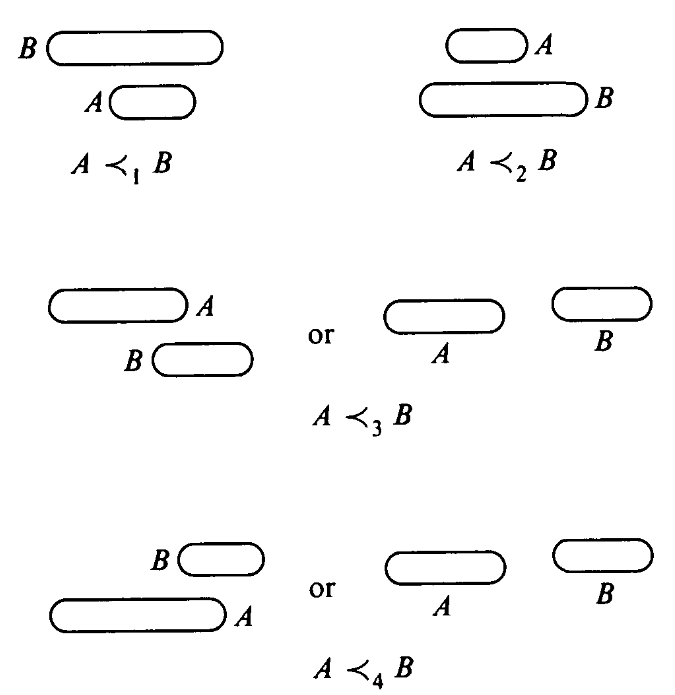
\includegraphics[scale=0.3]{14-1.png}
        \caption{An illustration of relations $<_1,<_2,<_3,<_4$.}
        \label{fig:14-1}
    \end{figure}
    We can check these relations are well defined and that if there exists two disjoint planner convex sets, then they must satisfy one of these four relations.

    We use Dilworth's Theorem on $(P_1=\mathcal{C},<_1)$, there is either a chain (which means pairwise disjoint sets, then we are done) of size $\geq n^\frac{1}{5}$ or an antichain $A_1$ of size $\geq n^\frac{4}{5}$.
    
    If there is no chain of size $\geq n^\frac{1}{5}$ in $(P_1=\mathcal{C},<_1)$, we use Dilworth's Theorem on $(A_1,<_2)$, there is either a chain (which means pairwise disjoint sets, then we are done) of size $\geq n^\frac{1}{5}$ or an antichain $A_2$ of size $\geq n^\frac{3}{5}$.

    If there is no chain of size $\geq n^\frac{1}{5}$ in $(A_1,<_2)$, we use Dilworth's Theorem on $(A_2,<_3)$, there is either a chain (which means pairwise disjoint sets, then we are done) of size $\geq n^\frac{1}{5}$ or an antichain $A_3$ of size $\geq n^\frac{2}{5}$.

    If there is no chain of size $\geq n^\frac{1}{5}$ in $(A_2,<_3)$, we use Dilworth's Theorem on $(A_3,<_4)$, there is either a chain (which means pairwise disjoint sets, then we are done) of size $\geq n^\frac{1}{5}$ or an antichain $A_4$ of size $\geq n^\frac{1}{5}$. $A_4$ is an antichain in every poset, so it is pairwise intersecting. In conclusion, we have proved there exists no less than $n^\frac{1}{5}$ many of them that are pairwise intersecting or pairwise disjoint.

    For the upper bound $n^{\log2/\log5}$, we construct $C_5^{(i+1)}$ by Iterating blowup every point of $C_5^{(i)}$ to $C_5$, where $C_5^{(1)}=C_5$. We can check $C_5^{(t)}$ has $n=5^t$ points and the size of its largest clique and independent set is $2^t=n^{\log2/\log5}.$ Now we need to check this is the intersection graph of some $n$ convex sets $\mathcal{C}$ in the plane $\mathbb{R}^2$.\footnote{The following is copied from \cite{LarmanDavidet1994}} We choose segments as convex sets, For any two points $p,q$ and any $\varepsilon>0$,there exists five segments $p_1q_1,p_2q_2,...,p_5q_5$ such that $p_iq_i$ intersects only the segments $p_{i-1}q_{i-1}$ and $p_{i+1}q_{i+1},$ and all $p_i$ (all $q_i$) are inside the circle around $p(q)$ with radius $\varepsilon$ (the indices are taken mod 5). See Figure\ref{fig:14-2}\footnote{This picture is copied from \cite{LarmanDavidet1994}}.
    \begin{figure}[H]
        \centering
        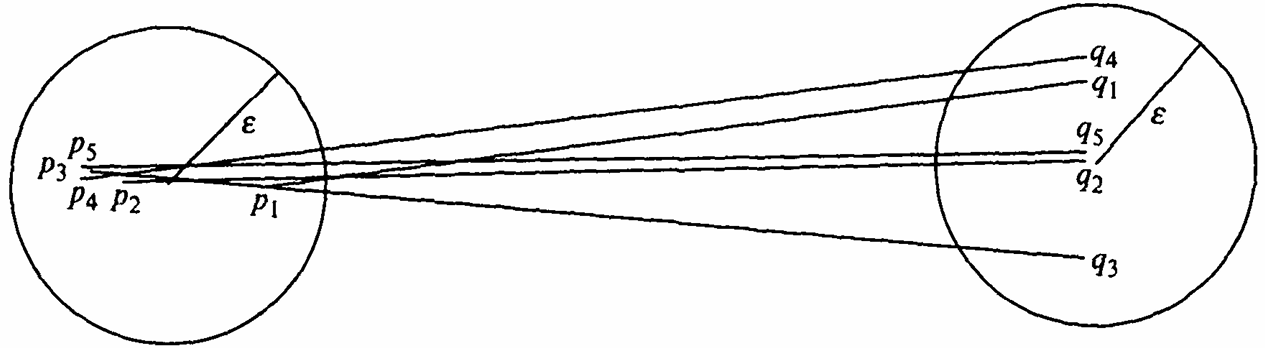
\includegraphics[scale=0.3]{14-2.png}
        \caption{A representation of the 5-cycle by segments}
        \label{fig:14-2}
    \end{figure}
     Let $C_5^{(1)}$ be such a family of five segments. Given $C_5^{(i)}$, choose $\varepsilon$ to be so small that no disk of radius $\varepsilon$ around an endpoint of a segment of $C_5^{(i)}$ meets any other segment of $C_5^{(i)}$. To obtain $C_5^{(i+1)}$, replace each segment of $C_5^{(i)}$ by a family of five segments satisfying the conditions of the construction. We can check this construction satisfis our need.
\end{proof}

\begin{remark}
    Cannot hope for any $\omega(\log n)$ bound for intersection graph of convex sets in $\mathbb{R}^3.$ Because by the result of Tietze, every graph can be realized as intersection graph of convex sets in $\mathbb{R}^3.$ 
\end{remark}

\begin{exercise}
    Prove that for any two disjoint convex set $A,B$ in $\mathbb{R}^2$, there exists $i\in [4]$, such that $A<_iB$
\end{exercise}

\begin{exercise}
    Prove that for all $i\in [4]$, $<_i$ is transitive.
\end{exercise}

\newpage

\section{Lecture 15:Ramsey via Dilworth \&  Erd\''os-Rado's sunflower lemma}
\subsection{Axis-aligned boxes}
\begin{definition}
   An axis-aligned box in $R^d$ is the sets  of the form $K=K_1\times\cdots\times K_d$, where $K_i\subset\mathbb{R} $ is a closed interval, for $i\in [d]$, where $[d]=\{1,2,...,d\}$.
\end{definition}
\begin{definition}
    $b(n,d)$ equals to the maximal number of $m$, s.t  $\forall$ $n$ boxes in $\mathbb{R}^d$, $\exists$ $m$ of them that are either pairwise intersecting or pairwise disjoint.
\end{definition}
In the intersection graph of the $n$ boxes, cliques stand for those pairwise intersecting boxes and independent sets stand of those pairwise disjiont boxes.

\begin{theorem}[Tomon\cite{tomon2022lower}]
    $\frac{\Omega(\sqrt{n})}{(\log n)^{\frac{d-2}{2}} 
\cdot  \log\log n}   \leq b(n,d)\leq O(\sqrt{n})\cdot (\frac{\log\log n}{\log n})^{\frac{d-2}{2}}$.
\end{theorem}

 For rectangles in the plane, the above theorem is $\frac{\Omega(\sqrt{n})}{\log\log n}  \leq b(n,2)\leq O(\sqrt{n})$. One open problem is that can 
 we close the gap between the upper bound and lower bound ?
\begin{theorem}[Larman-Matous$\breve{e}$k-Pach-T$\Ddot{o}$or$\Ddot{o}$csik]\label{thm15.4}
    $b(n,2)\geq \Omega(\sqrt{\frac{n}{\log n}})$.
\end{theorem}
Theorem \ref{thm15.4} is actually that for all $n$ axis-aligned rectangles in the plane $\mathbb{R}^2$, there exists $\Omega(\sqrt{\frac{n}{\log n}})$ many of them that are pairwise intersecting or disjoint.


\textbf{Idea of the proof }
  \begin{enumerate}
        \item Dilworth' theorem.

        \item Induction.

        \item Divide \& conquer.
    \end{enumerate}
 The "Divide \& conquer" idea is that we divide the whole into several pieces and conquer those pieces (usually by Induction).

 \begin{proof}[proof of theorem\ref{thm15.4}]
   Let $G$ be the intersecting graph .It suffices to prove that $\forall$ $k$ and $\forall$ $n= k\cdot 2^k$, $n$ is the number of rectangles, we have the following holds,
\begin{equation*}
    \omega(G)\cdot\alpha(G)\geq 2^k \approx \frac{n}{\log_2 n}.
\end{equation*}
This is because those pairwise intersecting rectangles and independent sets stand of those pairwise disjiont rectangles.

Let$R$ be the set of those rectangles. Now we start to induction on $k$. Basic situation $k=1$,  $n=2$, this is trivial situation.

Inductive step: By perturbing the rectangles if necessary we may assume all the lines containing some right vertical line segment of a rectangle are distinct, which give a order of rectangles. (A rectangle $R_1$ is less than $R_2$  in the ordering if the corresponding line of $R_1$ is in the left of the corresponding line of $R_2$)

Let $l$ is the  $((k-1)2^{k-1}+1)$-th  line  in those lines which contains some right vertical line segment of a rectangle and $R_0\subseteq R$ be the set of all rectangles intersecting the line $l$. 

Two rectangles in $R_0$ are intersecting if and onle if  their projections on $l$ are interesing are intersecting. So we can consider the interval graph $G_0$ for $R_0$.

If $|R_0| = 2^k$, by the conclusion in interval graphs, we have 
\begin{equation*}
     \omega(G)\cdot\alpha(G)\geq \omega(G_0)\cdot\alpha(G_0)   \geq 2^k.
\end{equation*}
So we assume $|R_0|<  2^k$. Let $R_1\subseteq R$ be the set of all rectangles to the left of the line $l$.(i.e  the first $(k-1)2^{k-1}$ in the above ordering.)

We now let $R_2=R\backslash (R_0\cup R_1)$, then $|R_2|\geq n-(k-1)2^{k-1}-2^k=(k-1)2^{k-1}$. Let $G_i$ is the intersecting graph of $R_i$, for $i=1,2$. By indction hypothesis, for $i=1,2$,
\begin{equation*}
    \omega(G_i)\cdot\alpha(G_i)   \geq 2^{k-1}.
\end{equation*}

Notice that the rectangles in $R_1$ is disjoint from rectangles in $R_2$, so we have $\alpha(G)\geq \alpha(G_1)+\alpha(G_2)$ and $\omega(G)\geq \max\{\omega(G_1),\omega(G_2)\}$. Then,
\begin{equation*}
    \omega(G)\cdot\alpha(G) \geq \max\{\omega(G_1),\omega(G_2)\}\cdot( \alpha(G_1)+\alpha(G_2))\geq \omega(G_1)\cdot\alpha(G_1)+\omega(G_2)\cdot\alpha(G_2)\geq 2^k
\end{equation*}
 \end{proof}
Next, we  introduce a related conjecture which is still open. View rectangles(boxes) as a set system(hypergraph) where each rectangle is a set in the set system(hyperedge in the hypergraph).
\begin{definition}
    Let $X$ be the ground set.  For a set system $\mathcal{F}\subseteq 2^X$, a set of points $T\subseteq X$ is a transversal of $\mathcal{F}$ if $\forall F \in \mathcal{F}$, $T\cap F\neq \emptyset$. The transversal number $\tau(\mathcal{F})$ is the size of smallest transversal of $\mathcal{F}$. Let $\nu (\mathcal{F})$ be its matching number, which is the size of largest pairwise disjoint sets in $\mathcal{F}$.
\end{definition}

\begin{proposition}
    For all set system $\mathcal{F}$, we have $\tau(\mathcal{F})\geq \nu (\mathcal{F})$
\end{proposition}
Let's see two examples.
\begin{example}
    Let $X=[7]$ and $\mathcal{F}$ is a collection of $3$-sets( in the following picture those sets are triangles with a red point). $\tau(\mathcal{F})=2$ and $\nu(\mathcal{F})=2$.
    \begin{figure}[H]
        \centering
        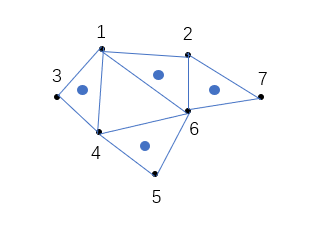
\includegraphics[scale=0.7]{15-1.png}
    \end{figure}
\end{example}

\begin{example}
    Let $X$ be all the point in $\mathcal{R}^2$ and $\mathcal{F}$ is the rectangles in the following picture. $\tau(\mathcal{F})=3$ and $\nu(\mathcal{F})=2$.
    \begin{figure}[H]
        \centering
        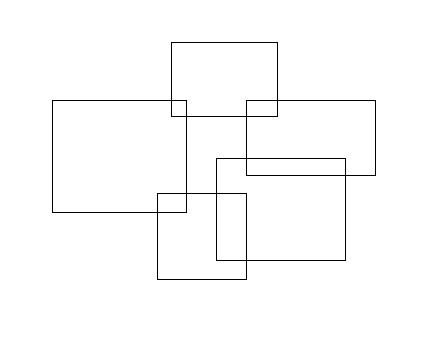
\includegraphics[scale=0.7]{15-2.png}
    \end{figure}
    
\end{example}

\begin{conjecture}[Gy\'arf\'es \& Lehel]\label{conj15.9}
    $\forall$ collection of axis-aligned rectangles $R$ in $\mathcal{R}^2$, we have
    \begin{equation*}
        \tau(R)=O(\nu(R)).
    \end{equation*}
\end{conjecture}
\begin{remark}
    Let $G$ be the intersection graph of $R$, then $\nu (R)=\alpha(G)$, $\tau(R)$ is the minimal number of disjoint cliques covering $V(G)$. It is easy to see $\omega(G)\geq \frac{n}{\tau(R)}$. So if the conjecture\ref{conj15.9} is true, then $\omega(G)\cdot\alpha(G) \geq \frac{n}{\tau(R)}\cdot \nu (R)= \Omega(n)$, which  also implies $b(n,2)\geq \sqrt{n}$
\end{remark}
Next theorem is the best bound of $\tau$ we know so for.
\begin{theorem}\cite{tomon2022lower}
Let $B$ be the collection of boxes in $\mathcal{R}^d$, $\nu=\nu(B)$, $\tau=\tau(B)$. We have
\begin{equation*}
    O(\nu)\cdot(\frac{\log \nu}{\log\log\nu})^{d-2}\leq \tau\leq O(\nu)\cdot (\log\nu)^{d-2}(\log\log\nu)^2
\end{equation*}
\end{theorem}

\subsection{Sunflower / $\Delta$-system}
\begin{definition}
    Let $r\in \mathcal{N}$, a sunflower($\Delta$-system) with kernel $K$ and $r$ petals is collection of sets $\{S_1,S_2,...,S_r\}$, s.t $\forall$ distinct $i,j\in [r]$, $S_i\cap S_j=K$. We call $S_i\backslash K$ the petals, $i\in [r]$.
\end{definition}

\begin{remark}
    Note that the kernal $K$ could be empty.
\end{remark}

\begin{example}
    This is a picture of sunflower with 5 petals and kernel $K$.
    \begin{figure}[H]
        \centering
        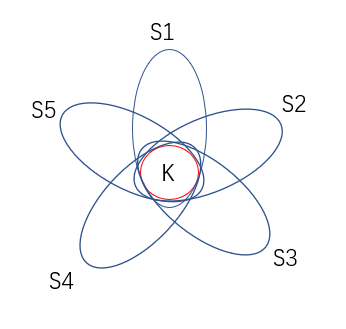
\includegraphics[scale=0.7]{15-3.png}
        \caption{A sunflower with 5 petals and kernel $K$}
    \end{figure}
\end{example}

\begin{remark}
    Sunflowers hanv many applications in Theoretical Computer Science.
\end{remark}
The following theorem tell us that if a collection of $k$-sets is large, we can find a large sunflower. One may need to mention is that the size of ground set does not play a role below. 

\begin{theorem}[\Erdos{} \& Rado\cite{Erds1961INTERSECTIONTF}]\label{thm15.16}
    $\forall$ $k\geq 1$, $\forall$ $\mathcal{F}$ a system of $k$-sets, if $|\mathcal{F}|>k!(r-1)^k$, we can find a sunflower with $r$ petals.
\end{theorem}

\begin{proof}[proof of theorem\ref{thm15.16}]
    Induction on $k$. Basic case $k=1$, $\mathcal{F}$ is a set of singletons.
    $|\mathcal{F}|>r-1$, so we have at least $r$ singletons. Each of singletons can be viewed as a petals. 

    Inductive step. Consider a maximum matching of $\mathcal{F}$, say $E_1,E_2,...,E_m$. We may assume $m\leq r-1$, or $r$ of them consists a sunflower with $r$ petals. The maximal proposition implies that $T:=\cup_{i\in [m]} E_i$ is a transversal of $\mathcal{F}$, i.e $\forall$ $F\in \mathcal{F}$, $F\cap T\neq \emptyset$. So, $|T|=m\cdot k\leq (r-1)k$. By Pigeonhole Theorem, there exist a point $x$ in $T$, such that the number of sets in $\mathcal{F}$, say those sets $\mathcal{F}_x$ ,containing is at least $\frac{|\mathcal{F}|}{|T|}> \frac{k!(r-1)^k}{(r-1)k}=(k-1)!(r-1)^{k-1}$ .

    Let $\mathcal{F}'=\{F\backslash \{x\}: F\in\mathcal{F}_x \}$ is a collection of (k-1)-sets with size larger than $(k-1)!(r-1)^{k-1}$, by induction hypothesis,  $\mathcal{F}'$ contains a sunflower with $r$ petals and kerner $K'$. Then we find a sunflower $\mathcal{F}_x$ with $r$ petals and kernal $K\cup {x}$. 

    
\end{proof}



\newpage
\section{Lecture 16: Harris-Kleitman correlation inequality}
\begin{definition}
    Define $f(k,r)$ as the minimum integer $m$ such that if any system of $k$-sets $\mathcal{F}$ has size at least $m$, then $\mathcal{F}$ contains a sunflower with $r$ petals.
\end{definition}
Then \Erdos{}- Rado theorem says $f(k,r) \leq k!(r-1)^k+1$. Here we can give a lower bound that $f(k,r) > (r-1)^k$ by considering the $k$-uniform complete $k$-partite hypergraph with each part of size $r-1$. Thus $\mathcal{F} = \{F: |F\cap V_i| =1, i\in [k]\}$, where each $V_i$ is the $i$-th part of $K_{r-1, \dots, r-1}^{(k)}$ of size $r-1$.

\begin{exercise}
    Show that such $\mathcal{F}$ has no sunflower with $r$ petals.
\end{exercise}

\begin{conjecture}[\Erdos{}- Rado sunflower conjecture, \cite{Erds1960IntersectionTF}]
    For each $r \geq 3$, there exists $C = C(r)$ such that $f(k,r) \leq C^k$.
\end{conjecture}

The recent breakthrough of this conjecture can be seen in \cite{Alweiss2019ImprovedBF} and \cite{Rao2019CodingFS} that $C = O(r\log(rk))$.

\subsection{Harris-Kleitman inequality}
\begin{definition}
    The family $\mathcal{F}$ of subsets of $[n]$ is $intersecting$ if members of $\mathcal{F}$ are pairwise intersecting, i.e., for every $F, F' \in \mathcal{F}$, we have $F \cap F' \neq \emptyset$.
\end{definition}

\begin{question}
    How large can an intersecting family be?
\end{question}

\begin{proposition}{}{}\label{prop16-1}
    Every intersecting family $\mathcal{F} \subseteq 2^{[n]}$ has at most $2^{n-1}$ members.
\end{proposition}
\begin{proof}
    By the definition of intersecting family, for each set $A \subseteq [n]$, only one of $A, \Bar{A} = [n]\backslash A$ could appear in $\mathcal{F}$. It's obviously that the number of such complementary pairs is $2^{n-1}$. Thus $\mathcal{F}$ misses at least $2^{n-1}$ members.
\end{proof}
\begin{remark}
    Proposition \ref{prop16-1} is tight. Here we give two tight examples: 
    
    Let $\mathcal{F}_1$ be the family of all sets that containing one fixed member.
    
    Suppose $n=2t+1$ is an odd number. Let $\mathcal{F}_2$ be the family of all sets of size at least $t+1$.
\end{remark}

\begin{definition}
    An intersecting family $\mathcal{F} \subseteq 2^{[n]}$ ia $maximal$ if any of its superfamily is not intersecting, i.e., for each subset $A \notin \mathcal{F}$, there exist $F \in \mathcal{F}$ such that $A \cap F = \emptyset$.
\end{definition}

\begin{exercise}
    Prove that all maximal intersecting family in $2^{[n]}$ are of size $2^{n-1}$.
\end{exercise}

\begin{question}
    What about the maximum size of $\mathcal{F}_1 \cup \mathcal{F}_2$ for intersecting families $\mathcal{F}_1$ and $\mathcal{F}_2$?
\end{question}

\begin{definition}
    A family of sets $\mathcal{D} \subseteq 2^{[n]}$ is a $down$-$set$ (simplicial complex) if it is closed under taking subsets. That is, if $T\in \mathcal{D}$ and $S\subseteq T$, then $S \in \mathcal{D}$.
    A family of sets $\mathcal{U} \subseteq 2^{[n]}$ is an $up$-$set$ if it is closed under taking supersets. That is, if $T\in \mathcal{U}$ and $S\supseteq T$, then $S \in \mathcal{U}$.
\end{definition}

\begin{theorem}[Harris-Kleitman inequality, \cite{KLEITMAN1966153}]{} \label{HK}
    Let $\mathcal{A}$ and $\mathcal{B}$ be down-sets in $2^{[n]}$. Then $$\frac{|\mathcal{A} \cap \mathcal{B}|}{2^n} \geq \frac{|\mathcal{A}|}{2^n} \cdot \frac{|\mathcal{B}|}{2^n}.$$
\end{theorem}
\begin{remark}
    Let $X$ be the random variable that sample the subset of $[n]$ uniformly at random. Then Harris-Kleitman inequality implies that $$\mathbb{P}r(X \in \mathcal{A} \cap \mathcal{B}) \geq \mathbb{P}r(X \in \mathcal{A}) \cdot \mathbb{P}r(X \in \mathcal{B}).$$

    If $\mathcal{A}$ and $\mathcal{B}$ are independent events, then the equal holds. Here Harris-Kleitman inequality is saying when both $\mathcal{A}$ and $\mathcal{B}$ are down-sets, event $\mathcal{A}$ and event $\mathcal{B}$ are positively correlated.
\end{remark}
This is intuitive because being both down-sets, they both favour small sets.

\begin{exercise}\label{ex16-2}
    \begin{itemize}
        \item Prove that if $\mathcal{A}$ and $\mathcal{B}$ are up-sets in $2^{[n]}$, then $$\frac{|\mathcal{A} \cap \mathcal{B}|}{2^n} \geq \frac{|\mathcal{A}|}{2^n} \cdot \frac{|\mathcal{B}|}{2^n}.$$

        \item Prove that if $\mathcal{A}$ is an up-set in $2^{[n]}$ and $\mathcal{B}$ is a down-set in $2^{[n]}$, then $$\frac{|\mathcal{A} \cap \mathcal{B}|}{2^n} \leq \frac{|\mathcal{A}|}{2^n} \cdot \frac{|\mathcal{B}|}{2^n}.$$
    \end{itemize}
\end{exercise}

\textbf{Notation}: Let $\mathcal{F}$ be a family of subsets of $[n]$. Fix any element $i \in [n]$, then we have the partition $\mathcal{F} = \mathcal{F}(i) \cup \mathcal{F}(\Bar{i})$, where $\mathcal{F}(i) = \{ F \in \mathcal{F}: i\in F \}$, $\mathcal{F}(\Bar{i}) = \{ F \in \mathcal{F}: i\notin F \}$.

For example, let $n=3$, $i=3$. We can seem $2^[n]$ as $\{0,1\}^n$. Now $\mathcal{F}(i)$ is the collection of all strings with $1$ on the $i$-th coordinate, and $\mathcal{F}(\Bar{i})$ is the collection of all strings with $0$ on the $i$-th coordinate. Thus the partition can be seen in figure \ref{fig:16-1}.
\begin{figure}[H]
        \centering
        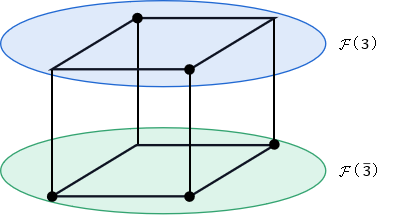
\includegraphics[scale=0.5]{16-1.png}
        \caption{Partition into two co-dimension-$1$ subcubes}
        \label{fig:16-1}
\end{figure}

\begin{proof}[Proof of Theorem \ref{HK}]
    Induction on $n$ to show $$2^n \cdot |\mathcal{A} \cap \mathcal{B}| \geq |\mathcal{A}| \cdot |\mathcal{B}|.$$

    The case $n=1$ can be easily checked. For $n > 1$, partition $\mathcal{A} = \mathcal{A}(\Bar{n}) \cup \mathcal{A}(n)$.  Define the link of $n$ in $\mathcal{A}$ be $$\mathcal{L}_{\mathcal{A}}(n) = \{F\backslash \{n\}: F \in \mathcal{A}(n) \}.$$
    Let $|\mathcal{L}_{\mathcal{A}}(n)|=|\mathcal{A}(n)|=a_1$, $|\mathcal{A}(\Bar{n})|=a_2$. Then $a_1+a_2=a=|\mathcal{A}|$. Do the same for $\mathcal{B}$ as above.

    Thus we have \begin{equation}\label{equ16-1}
        \begin{split}
            & 2^n \cdot |\mathcal{A} \cap \mathcal{B}| \\
            = & 2^n \cdot |\mathcal{A}(n) \cap \mathcal{B}(n)| + 2^n \cdot |\mathcal{A}(\Bar{n}) \cap \mathcal{B}(\Bar{n})|\\
            = & 2^n \cdot |\mathcal{L}_{\mathcal{A}}(n) \cap \mathcal{L}_{\mathcal{B}}(n)| + 2^n \cdot |\mathcal{A}(\Bar{n}) \cap \mathcal{B}(\Bar{n})|\\
            \overset{Inductive\ hypothesis}{\geq} & 2|\mathcal{L}_{\mathcal{A}}(n)|\cdot |\mathcal{L}_{\mathcal{B}}(n)| + 2|\mathcal{A}(\Bar{n})|\cdot |\mathcal{B}(\Bar{n})|\\
            = & 2a_1b_1+ 2a_2b_2
        \end{split}
    \end{equation}

    In order to achieve our goal, we give the following claim.

    \begin{claim}
        $\mathcal{L}_{\mathcal{A}}(n) \subseteq \mathcal{A}(\Bar{n})$, i.e. $a_1 \leq a_2$. So does $\mathcal{B}$.
    \end{claim}
    \begin{proof}
        For each $F \in \mathcal{L}_{\mathcal{A}}(n)$, we have $F \cup \{n\} \in \mathcal{A}$. So $F \in \mathcal{A}(\Bar{n})$ since $\mathcal{A}$ is a down-set in $2^{[n]}$.
    \end{proof}

    Now we have \begin{equation*}
        \begin{split}
            & 2^n \cdot |\mathcal{A} \cap \mathcal{B}| \geq |\mathcal{A}| \cdot |\mathcal{B}|\\
            \Leftrightarrow & 2a_1b_1+ 2a_2b_2 \geq ab=(a_1+a_2)(b_1+b_2) \\
            \Leftrightarrow & a_1b_1+ a_2b_2 \geq a_1b_2+ a_2b_1 \\
            \Leftrightarrow & (a_1-a_2)(b_1-b_2) \geq 0
        \end{split}
    \end{equation*}
    Thus complete the proof.
\end{proof}

\begin{remark}
    Harris-Kleitman inequality is optimal:
    
    Take disjoint sets of indices $A, B \subseteq [n]$. Let $\mathcal{A} = 2^{[n]\backslash A}$, $\mathcal{B} = 2^{[n]\backslash B}$. Both $\mathcal{A}$ and $\mathcal{B}$ are down-sets. Then $\mathcal{A} \cap \mathcal{B} = 2^{[n]\backslash (A\cup B))}$. Here the equal holds $$\frac{|\mathcal{A} \cap \mathcal{B}|}{2^n} = 2^{-(|A|+|B|)} = \frac{|\mathcal{A}|}{2^n} \cdot \frac{|\mathcal{B}|}{2^n}.$$
\end{remark}

\subsection{Applications of Harris-Kleitman inequality}
\begin{theorem}[Kleitman, 1966, \cite{KLEITMAN1966153}]\label{K1}
    For each sequence of intersecting families $\{\mathcal{F}_i \}_{i=1}^t$, $\mathcal{F}_i \subseteq 2^{[n]}, i\in [t]$, there is $$|\bigcup_{i \in [t]}\mathcal{F}_i| \leq 2^n - 2^{n-t}.$$
\end{theorem}
\begin{remark}
    Theorem \ref{K1} is optimal: For each $i\in [t]$, let $\mathcal{F}_i$ be the collection of all sets containing element $i$.
\end{remark}
\begin{proof}
    Here prove by induction on $t$. For $t=1$, it holds by Proposition \ref{prop16-1}.
    For $t >1$, we may assume each $\mathcal{F}_i$ is an up-set. Then $\mathcal{F}_i^c = 2^{[n]} \backslash \mathcal{F}_i$ is a down-set. 
    
    First note that $\bigcup_{i \in [t]}\mathcal{F}_i = 2^{[n]} \backslash (\bigcap_{i \in [t]}\mathcal{F}_i^c)$, so $$|\bigcup_{i \in [t]}\mathcal{F}_i| = 2^n - |\bigcap_{i \in [t]}\mathcal{F}_i^c|.$$
    Now we use Harris-Kleitman inequality and Proposition \ref{prop16-1} to give a lower bound of $|\bigcap_{i \in [t]}\mathcal{F}_i^c|$.

    \begin{equation}
        \begin{split}
            |\bigcap_{i \in [t]}\mathcal{F}_i^c| & = |(\bigcap_{i \in [t-1]}\mathcal{F}_i^c) \cap \mathcal{F}_t^c|\\
            & \overset{Theorem \ref{HK}}{\geq} |\bigcap_{i \in [t-1]}\mathcal{F}_i^c|\cdot |\mathcal{F}_t^c|/ 2^n\\
            & \overset{Induction\ hypothesis}{\geq} 2^{n-(t-1)}\cdot 2^{n-1}/ 2^n\\
            & = 2^{n-t}
        \end{split}
    \end{equation}

    Thus complete the proof.
\end{proof}

\begin{definition}
    For any family $\mathcal{F} \subseteq 2^{[n]}$, write $$\Bar{\mathcal{F}} := \{ [n]\backslash F: F \in \mathcal{F} \}.$$
\end{definition}
\begin{exercise}
    Prove that $\Bar{\mathcal{F}}$ is intersecting if and only if $F \cup F' \neq [n]$ for each $F, F' \in \mathcal{F}$.
\end{exercise}
\begin{theorem}[Kleitman]\label{K2}
    Given an intersecting family $\mathcal{F} \subseteq 2^{[n]}$. If $\Bar{\mathcal{F}}$ is also intersecting, i.e., $F \cup F' \neq [n]$ for each $F, F' \in \mathcal{F}$, then $|\mathcal{F}| \leq 2^{n-2}$.
\end{theorem}
\begin{remark}
    Theorem \ref{K2} is tight: Let $\mathcal{F}$ be the collection of all sets containing element $1$ but not containing element $2$.
\end{remark}
\begin{proof}
    Let $\mathcal{F}^+$ and $\mathcal{F}^-$ be the upward and downward closure of $\mathcal{F}$ respectively. That is, $$\mathcal{F}^- = \{A: A\subseteq F\in \mathcal{F}\};$$ $$\mathcal{F}^+ = \{B: B\supseteq F\in \mathcal{F}\}.$$
    It's obviously that $\mathcal{F}\subseteq \mathcal{F}^+\cap \mathcal{F}^-$.

    For each $F,F' \in \mathcal{F}$, there are $F \cap F' \neq \emptyset$ and $F \cup F' \neq [n]$. In addition, by the definition of $\mathcal{F}^+$ and $\mathcal{F}^-$, it's easy to check that $\mathcal{F}^+$ and $\Bar{\mathcal{F}^-}$ are all intersecting. So $|\mathcal{F}^+| \leq 2^{n-1}$, $|\Bar{\mathcal{F}^-}| = |\mathcal{F}^-| \leq 2^{n-1}$
    
    Finally, by Harris-Kleitman inequality (Exercise \ref{ex16-2}), we have $$|\mathcal{F}| \leq |\mathcal{F}^+\cap \mathcal{F}^-| \leq \frac{1}{2^n}|\mathcal{F}^+|\cdot|\mathcal{F}^-| \leq 2^{n-2}.$$

    Thus complete the proof.
\end{proof}

\newpage
\section{Lecture 17}
\subsection{Katona's proof of \Erdos{}-Ko-Rado Theorem}
\begin{definition}
For positive integer $n \ge k > 0$, a system of $k$-sets is $k$-unifrom family on ground set $[n]$, i.e.$\mathcal{F}\subseteq \binom{[n]}{k}$. $\binom{[n]}{k}$ is all k-subsets of $[n]$.
\end{definition}

\begin{definition}
    $\mathcal{F}$ is an intersecting family, if $\forall F,F'\in \mathcal{F}$ satisfy $F\cap F' \ne \emptyset$
\end{definition}

We know that if $\mathcal{F}$ is a intersecting family without k-uniform condition, we have $|\mathcal{F}|\le 2^{n-1}$. According to the definitions, there is the following question, naturally. 

\begin{question}
How large can a k-uniform intersecting family be? 
\end{question}
It is easy for us to gain the following results.
\begin{itemize}
    \item $\mathbf{n<2k}$: Every two k-set are intersecting, so $\underset{\mathcal{F}}{max}|\mathcal{F}|=\binom{n}{k}$. 
    \item $\mathbf{n=2k}$: For each k-set $A\subset [n]$, $A$ and $\bar A$ we can choose at most one of their to form k-uniform intersecting family, so $\underset{\mathcal{F}}{max}|\mathcal{F}|=\frac{1}{2}\binom{n}{k}=\binom{n-1}{k-1}$.
    \item $\mathbf{n>2k}$: If all the k-sets in $k$-uniform family $\mathcal{F}$ have a common element. Obviously, $\mathcal{F}$ is an intersecting family. Let's counting the size of $\mathcal{F}$, we have $\underset{\mathcal{F}}{max}|\mathcal{F}|\ge \binom{n-1}{k-1}$.
\end{itemize}
For the upper bound of $k$-uniform intersecting family, it was given by \Erdos{}, Ko and Rado\cite{erdos1961intersection} in 1961. And we will give Katona's proof\cite{katona1964intersection} of following theorem. 

\begin{theorem}[\Erdos{}-Ko-Rado Theorem\cite{erdos1961intersection}, 1961] \label{EKRthm} 
    For $\forall n \ge 2k$, if $\forall \mathcal{F}\subseteq \binom{[n]}{k}$ is intersecting family. Then we have $$\underset{\mathcal{F}}{max}|\mathcal{F}|\ge\binom{n-1}{k-1}.$$
\end{theorem}
\begin{proof}
Let $C_n$ be all cyclic permutation of [n], so we have $|C_n|=(n-1)!$. Double count the pair $(\sigma, F)$ where $\sigma \in C_n$ and $F\in \mathcal{F}$ such that $F$ forms an interval is an arc in $\sigma$. Let $P$ be the number of the pairs $(\sigma, F)$.
\begin{claim}
    $|\mathcal{F}|k!(n-k)!=P\le (n-1)!k$.
\end{claim}
\begin{proof}
    For the first equality, from the point of view of $F\in \mathcal{F}$, we have that the number of the choices for $F$ is $|\mathcal{F}|$; the number of the way permutation $F$ is $k!$; the number of the way to permute $[n]\setminus F$ is $(n-k)!$. Multiply the above three numbers and we will gain the first equality.

    For the second inequality, from the point of view of $\sigma\in C_n$, we suffices to show that $\forall \sigma \in C_n$, Let $A_{\sigma}$ be the set of k-arcs in $\sigma$, then we have $|\mathcal{F}\cap A_{\sigma}|\le k$.
    
    Let's fix a set $F\in \mathcal{F}\cap A_{\sigma}$ and $F=\{x_1,...,x_k\}$. Let $E_i$ be the arc which ends at $x_i$ in $\sigma$ and $S_i$ be the arc which starts at $x_i$ in $\sigma$. Acccording to the condition, $\mathcal{F}$ is intersecting, then all sets in $A_{\sigma}\cap\mathcal{F}$ have to intersecting $F$. Therefore, they have to be one of the subsets of $\{E_1,...,E_k,S_1,..,S_k\}$. It is observed that for each pair  $\{E_i, S_{i+1}\}$, $\mathcal{F}$ can have at most one from these $(k-1)$ disjoint pair and $F=E_k=S_1$. Therefore, $P\le (n-1)!k$.
\end{proof}

Due to the above claim, we have
$$|\mathcal{F}|\le \frac{(n-1)!k}{k!(n-k)!}=\binom{n-1}{k-1}.$$
\end{proof}

\begin{remark}
When $n=2k$, extremal forms are $\frac{1}{2}\binom{n}{k}$ complementary pairs or stars. When $n>2k$, stars are the only extremal one.
\end{remark}

\begin{exercise}
    Prove that $n>k$, stars are the only $k$-uniform intersecting family of size $\binom{n-1}{k-1}$.
\end{exercise}
However, we also can rephrase Kotona's proof in a probabilistic way. The details are as follows.

\begin{proof}[Proof theorem \ref{EKRthm} in probabilistic way]
Sample $\sigma\in C_n$, let's consider arcs $A_{\sigma}$ in $\sigma$.
On one hand, $\forall \sigma \in C_n$, we have 
\begin{align}\label{eq1}
   |\mathcal{F}\cap A_{\sigma}|\le k .
\end{align}

On the other hand, Let's compute the expectation of $|\mathcal{F}\cap A_{\sigma}|$. As $\sigma\in C_n$ is uniform chosen and all $k$-sets in $\binom{[n]}{k}$ appears as an arc in $\sigma$ with the same probability, so we have
\begin{align}\label{eq2}
\mathbb{E}(|\mathcal{F}\cap A_{\sigma}|)=\underset{A\in A_{\sigma}}{\sum}Pr(A\in \mathcal{F})\overset{linearity~of~expectation}{=}n\frac{|\mathcal{F}|}{\binom{n}{k}}.
\end{align}
Take \eqref{eq1} and \eqref{eq2} together, we get $|\mathcal{F}|\le\binom{n-1}{k-1}.$
\end{proof}

we can get a recipe for upper bound a family $\mathcal{A}$ of discrete objects from the proof of theorem \ref{EKRthm}.
Given target group $\mathcal{A}$ (i.e. $\mathcal{A}$ in EKR theorem), let's find a contral group $\mathcal{B}$ (i.e. $\mathcal{A_\sigma}$) satisfying the following two conditions.
\begin{itemize}
    \item $\forall b \in \mathcal{B}$ distributes uniformly over something (i.e. $A_\sigma \supset A \sim \binom{[n]}{k}$), then we can confirm $Pr(b\in \mathcal{A})$ by measure of $A$ in probabilistic space (i.e. normalised counting measure $\mu (F)=\frac{|\mathcal{A}|}{\binom{n}{k}}$), such that $\mathbb{E}(|\mathcal{A}\cap\mathcal{B}|)=\underset{b\in \mathcal{B}}{\sum}Pr(b\in\mathcal{A})=\mu(A)|\mathcal{B}|$.
    \item $\forall \mathcal{B}$, we have $|\mathcal{A}\cap\mathcal{B}|$ can be bounded by a small number, i.e. $\mu(A)\le \frac{s}{|\mathcal{B}|}$.
\end{itemize}

Besides, we can phrasing EKR theorem \ref{EKRthm} in terms of Kneser graphs. 
\begin{definition}[Kneser Graph]
    Let $KG(n,k)=(V,E)$ be a graph with $V=\binom{[n]}{k}$ and $\forall S,T\in V$, $S\sim T$ if and only if $S\cap T=\emptyset$, i.e. kneser graph $KG(n,k)$ is the disjointness graph of $k$-sets in $[n]$.
\end{definition}
According to the definition, intersecting family $\mathcal{F}\in \binom{[n]}{k}$ and independent sets in $KG(n,k)$ are one-to-one. By EKR theorem\ref{EKRthm}, we have that $\forall n\ge 2k$, we have $\alpha(KG(n,k))\le \binom{n-1}{k-1}$.
\subsection{Counting the number of intersecting family}
\begin{definition}
    $\mathcal{F}\subseteq \binom{[n]}{k}$ is maximal intersecting if it is pairwise intersecting and $\forall \mathcal{F}'\supsetneqq \mathcal{F}$ is not intersecting.
\end{definition}
Obviously, as subfamily of an intersecting family are also intersecting, the number of $k$-uniform intersecting form at least $2^{\binom{n-1}{k-1}}$ (consider the all subfamilies of a star).

\begin{theorem}[J\'ozsef Balogh, Shagnik Das et al.\cite{balogh2015intersecting} 2014]
    $\forall n\ge 2k+1$, Let $A_k$ be the number of $k$-uniform intersecting family, then $A_k=2^{(1+o(1)\binom{n-1}{k-1}}$.
\end{theorem}

\begin{remark}
    when $n\ge 2k+1$, it is the optimal bound.
\end{remark}

\begin{exercise}
    Prove that there are exponentially at least $3^{\binom{n-1}{k-1}}$ many intersecting family when $n=2k$.
\end{exercise}

\begin{theorem}[J\'ozsef Balogh, Shagnik Das et al.\cite{balogh2015intersecting} 2014]\label{maxIntersecting} 

Let $M_k$ be the number of maximal intersecting $k$-uniform family on $n$, then 
$$M_k\le \underset{i=0}{\overset{\binom{2k}{k}}{\sum}}{\binom{\binom{n}{k}}{i}}\le \binom{n}{k^{\binom{2k}{k}}}$$
\end{theorem}

\begin{remark}
    Let's think of the bound of $k$-uniform, when $n$ grows. For the number of total intersecting families is exponential. And for the number of maximal intersecting families is polynomial. 
\end{remark}

\begin{definition}
    $\forall \mathcal{F} \subseteq \binom{[n]}{k}$, let $\mathcal{I}(\mathcal{F}):=\{G\in\binom{[n]}{k}:~G\cap F \ne \emptyset \forall F\in \mathcal{F}\}$ be the family of all k-set that intersect all sets in $\mathcal{F}$.
\end{definition}

According to the definition, we can gain the following observation. 

\begin{observation}
    $\mathcal{F}$ is intersecting, if and only if $\mathcal{F}\subseteq \mathcal{I}(\mathcal{F})$.
\end{observation}

\begin{exercise}\label{exer}
    $\mathcal{F}$ is maximal intersecting, if and only if $\mathcal{F}=\mathcal{I}(\mathcal{F})$.
\end{exercise}

\begin{observation}
    If $\forall \mathcal{F^{-}} \subsetneqq \mathcal{F}$, then we have $\mathcal{I}(\mathcal{F}^-)\supseteq \mathcal{I}(\mathcal{F})$ 
\end{observation}

\begin{lemma}
    Given a maximal intersecting family $\mathcal{F}\subseteq \binom{[n]}{k}$, then there exist a generating set $\mathcal{G}\subseteq \mathcal{F}$ such that $\mathcal{G}(\mathcal{G})=\mathcal{F}$.
\end{lemma}
\begin{proof}
    Initially, by exercise \ref{exer}, we have $\mathcal{F} =\mathcal{I}(\mathcal{F})$.

    delete sets one by one from $\mathcal{F}_0=\mathcal{F}$. Therefore, $\mathcal{F}_0\supseteq \mathcal{F}_0\supseteq\mathcal{F}_1\supseteq\mathcal{F}_2\supseteq...$. And according to the observation, we have $\mathcal{F}=\mathcal{I}(\mathcal{F}_0)\subseteq\mathcal{I}(\mathcal{F}_1)\subseteq\mathcal{I}(\mathcal{F}_2)\subseteq ...$. 

    Thus, there exists a generating set $\mathcal{G}$ of $\mathcal{F}$.
\end{proof}

The idea of theorem\ref{maxIntersecting} proof is as follows.
$\forall \mathcal{F}$ with maximal intersecting are able to map generating set $\mathcal{G}$ of $\mathcal{F}$ injectively. so we shall prove the following claim.
\begin{claim}
    $\forall \mathcal{F}$ is maximal intersecting family, there is exist a generating set $\mathcal{G}\subseteq \mathcal{F}$ of size at most $\binom{2k}{k}$.
\end{claim}

\newpage
\section{Lecture 18}



\newpage
\section{Lecture 19}



\newpage
\section{Lecture 20}

\subsection{Three proofs of Sauer-Shelah lemma}
\begin{definition}[VC dimension]
    Let $\mathcal{F} \subseteq 2^X$ be a set system on the ground set $X$. For $S \subseteq X$, the \emph{trace} of $\mathcal{F}$ on $S$ is $\mathcal{F}|_{S} := \{ F \cap S: F \in \mathcal{F} \}$. A set $S$ is \emph{shattered} by $\mathcal{F}$ if $\mathcal{F}|_{S} = 2^S$. In other words, for any $S' \subseteq S$, there exists $F \in \mathcal{F}$ s.t. $F\cap S = S'$. The \emph{VC dimension} of $\mathcal{F}$ is the size of the largest set $S \subseteq X$ shattered by $\mathcal{F}$.
\end{definition}

\begin{example}
Let $X$ be $\mathbb{R}^1$, and $\mathcal{F}$ be all closed intervals in $\mathbb{R}$.
\end{example}
\begin{claim}
    The VC dimension of $\mathcal{F}$ is 2. 
\end{claim}
\begin{proof}
    For the lower bound, we need to find a shattered 2-set. Indeed, take any 2 points in $\mathbb{R}$ such as $\{5,14\}$, it is easy to find four closed intervals which intersect $\{5,14\}$ with $\{\varnothing\},\{5\},\{14\},\{5,14\}$ respectively. For the upper bound, we need to show that for every 3-set $S$, it can not be shattered by $\mathcal{F}$, that is, there exists some $S'\subseteq S$ such that there is no $F \in \mathcal{F}$ satisfies $F\cap S=S'$. For example, let $S=\{5,14,2024\}$, we have $S'=\{5,2024\}$.
\end{proof}
But closed convex sets in higher dimension, already in $\mathbb{R}^2$, have infinite VC dimension.

\begin{example}
Let $X$ be $\mathbb{R}^2$, and $\mathcal{F}$ be all convex sets in $\mathbb{R}^2$.
\end{example}
\begin{claim}
    The VC dimension of $\mathcal{F}$ is infinite. That is, for every $n\in \mathbb{N}$, we can find an $n$-point set shattered by $\mathcal{F}$.
\end{claim}
Indeed, consider $n$ points lie on a cycle, for any subset $S'$ of this $n$-point set $S$, there exists a convex set intersecting $S$ with $S'$, see the following picture. 

\begin{figure}[H]
        \centering
        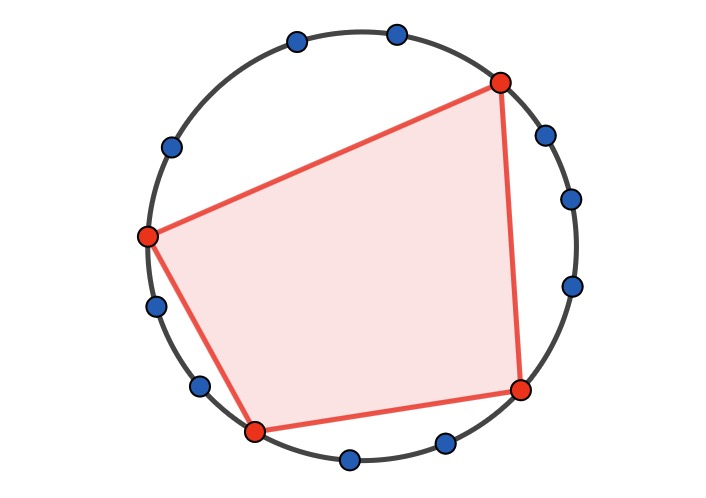
\includegraphics[scale=0.2]{20-1.jpg}
        \label{fig:20-1}
\end{figure}

\begin{example}
Consider half spaces in $\mathbb{R}^2$, that is, $X=\mathbb{R}^2$, $\mathcal{F}=$ all half spaces. Then the VC domension of $\mathcal{F}$ equals to 3.  
\end{example}
Indeed, it is at least 3 as illustrated in Figure \ref{fig:20-2}(a). It is less than 4: if the 4 points are in convex position, then the two sets of diagonal pairs cannot be separated; while if one point is in the convex hull of the others, then that point cannot be separated from the rest, see Figure \ref{fig:20-2}(b).
\begin{figure}[H]
        \centering
        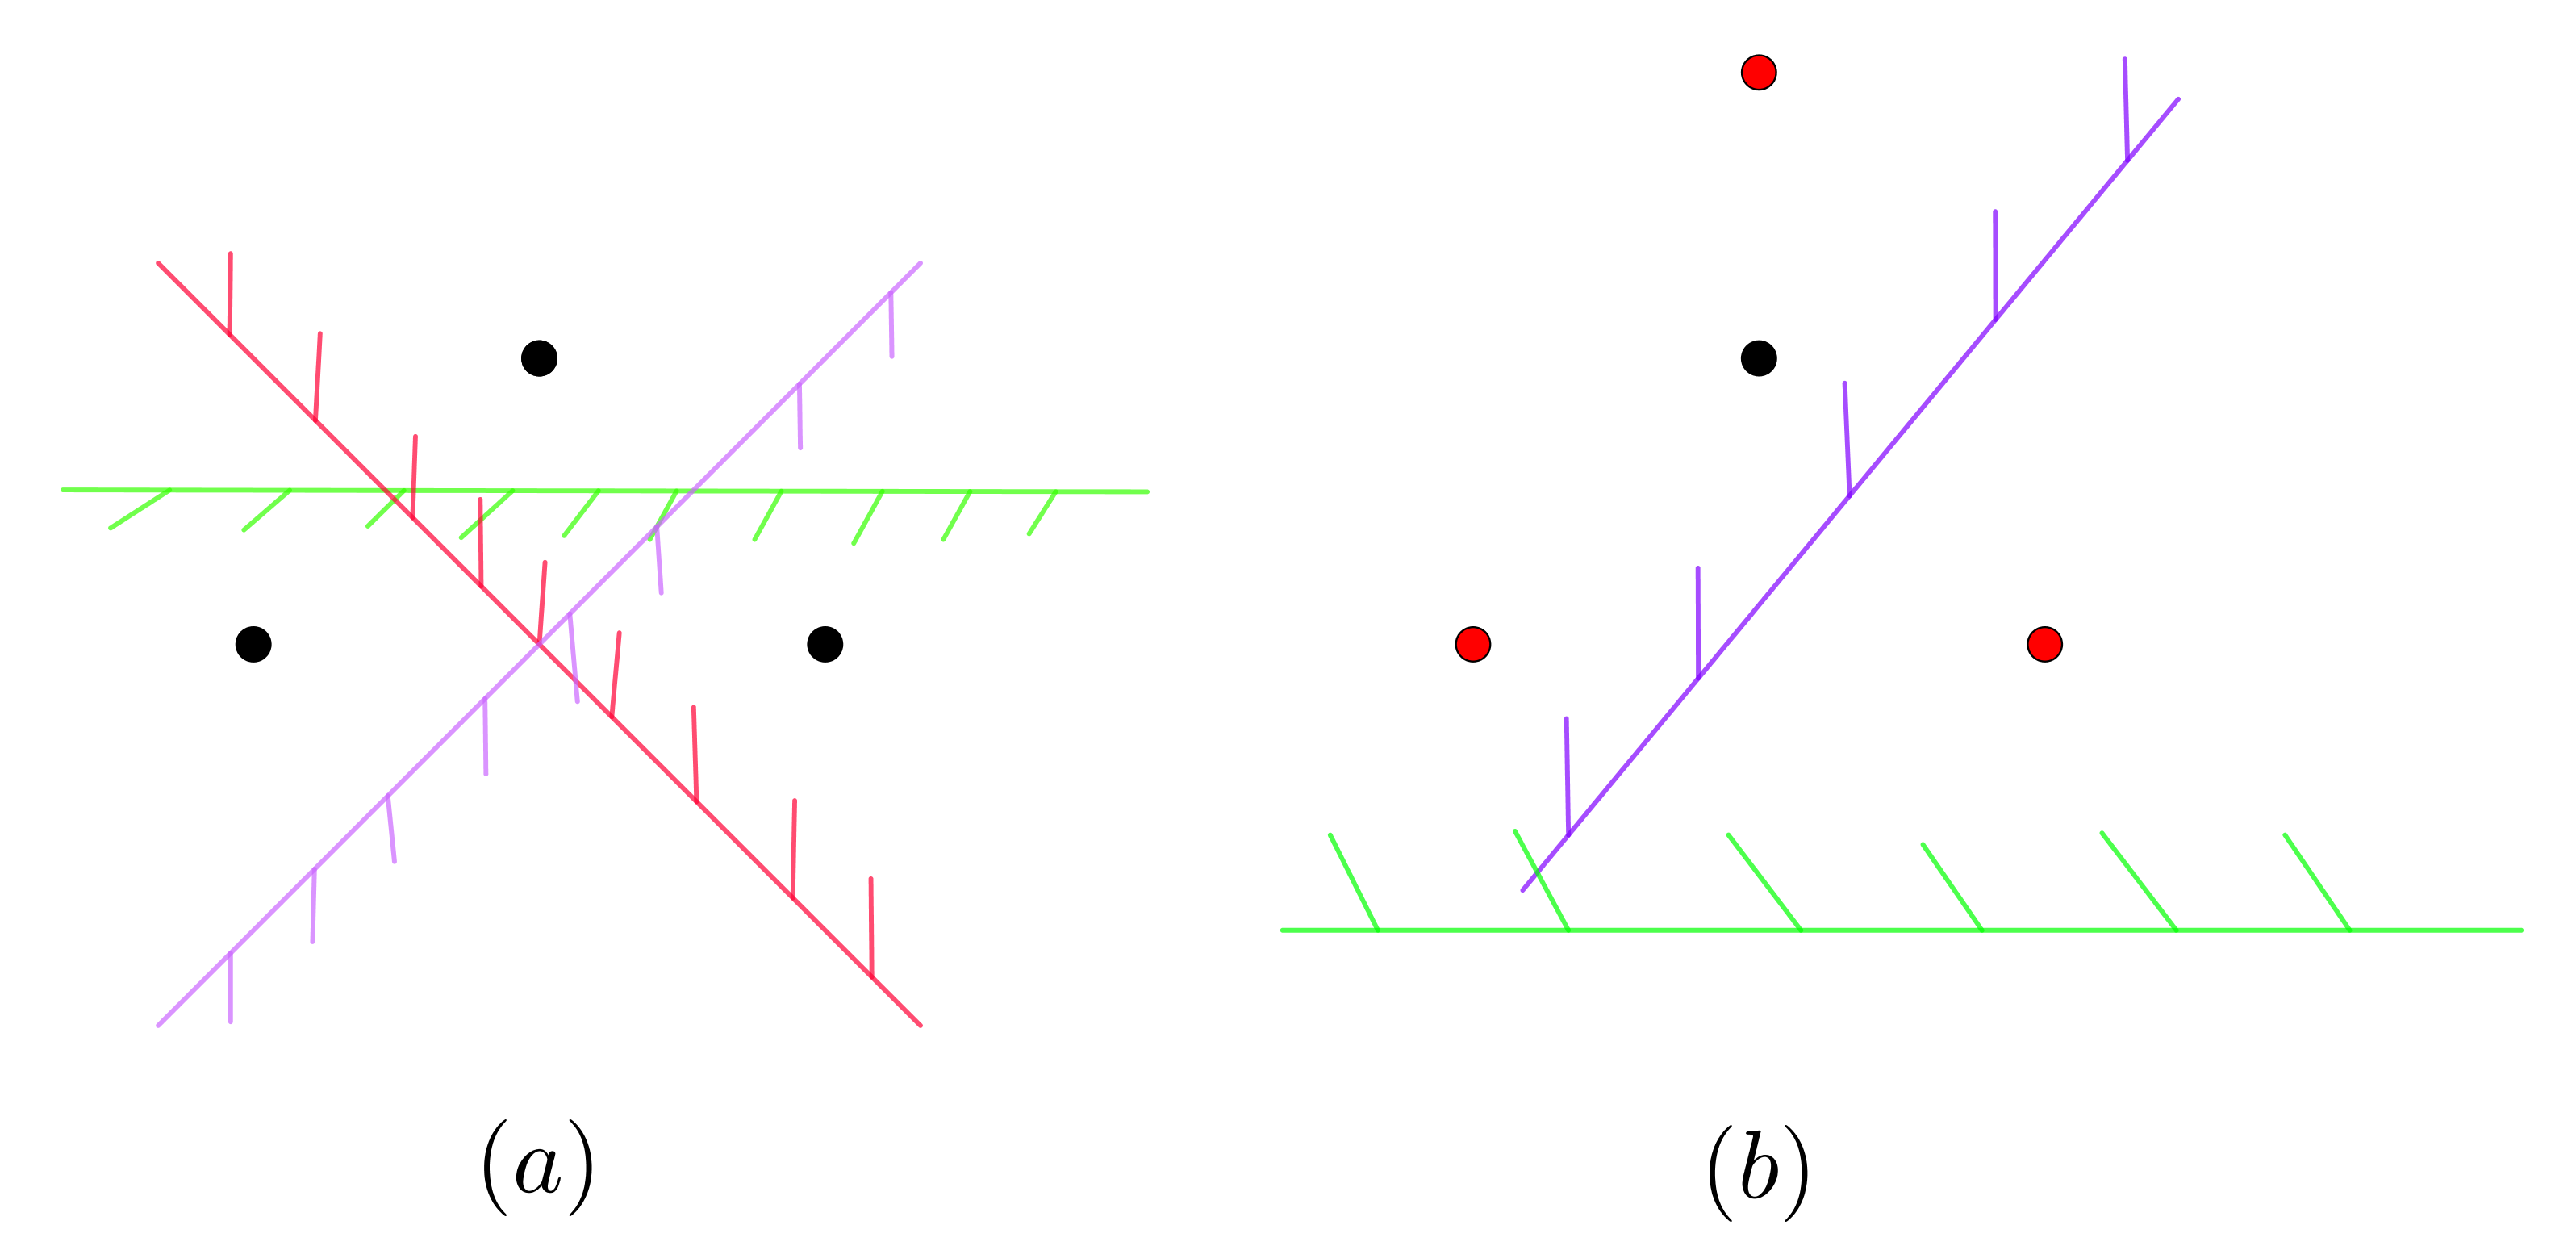
\includegraphics[scale=0.3]{20-2.jpg}
        \caption{$X=\mathbb{R}^2$, $\mathcal{F}=$ all half spaces}
        \label{fig:20-2}
\end{figure}


 \begin{exercise}
    Let $X=\mathbb{R}^2$, $\mathcal{F}=$ all axis-aligned rectangles. Prove that the VC domension of $\mathcal{F}$ equals to 4.
    \begin{figure}[H]
        \centering
        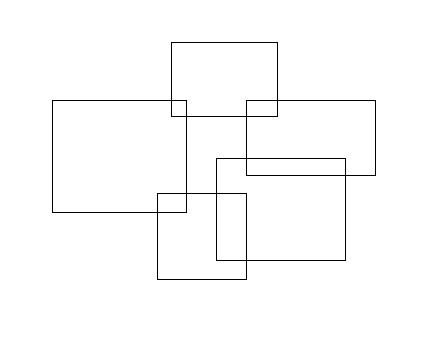
\includegraphics[scale=0.5]{15-2.png}
    \end{figure}
\end{exercise}

\begin{example}
    Given ground set $V = [n]$, let $\mathcal{F} = \binom{[n]}{n/2}$. We claim that any $\frac{n}{2}$-set in $[n]$ is shattered by $\mathcal{F}$. Then the VC-dimension of this set system is $\frac{n}{2}$.
\end{example}


\begin{lemma} [Sauer-Shelah~\cite{sauer1972density,shelah1972combinatorial}]\label{F}
    Let $\mathcal{F}\subseteq 2^{[n]}$ with VC dimension $d$, then $|\mathcal{F}|\leq \binom{n}{0}+\binom{n}{1}+\cdots+\binom{n}{d}$.
\end{lemma}

\begin{remark}
The bound is optimal.
\end{remark}

\begin{remark}
The Sauer-Shelah lemma in fact is slightly stronger: it bounds size of traces of $\mathcal{F}$ on any set. That is, for any $\mathcal{F}\subseteq 2^{[n]}$ with VC dimension $d$ and any $S\subseteq X$ of size $m$, then we have $|\mathcal{F}|_{S}|\leq \binom{m}{0}+\binom{m}{1}+\cdots+\binom{m}{d}$. We get this version from Sauer-Shelah lemma for free as the VC dimension of $\mathcal{F}|_{S}$ is no more than that of $\mathcal{F}$.
\end{remark}


\begin{proof}[Proof of Lemma~\ref{F}]
    By induction on $d$ and $n$, the base case for $d$ is easy. We fix $d$ first, the base case $n=d$ is trivial. We restrict $\mathcal{F}$ to $[n-1]$, let $\mathcal{F}_{1}=\mathcal{F}|_{[n-1]}=\{ F\backslash \{ n \} :F\in \mathcal{F} \}$. Note that $\mathcal{F}_{1}$ might not be $\mathcal{F}$. Let $\mathcal{F}_{2}=\{ F\in \mathcal{F}: n\notin F, F\cup\{ n \} \in \mathcal{F} \}$. Then $|\mathcal{F}|=|\mathcal{F}_{1}|+|\mathcal{F}_{2}|$. We claim that $\VC(\mathcal{F}_{2})\leq d-1$. In fact, if $A\subseteq [n-1]$ shattered by $\mathcal{F}_{2}$, then $A\cup \{ n \}$ shattered by $\mathcal{F}$. By induction on $n$, we have
    \begin{equation*}
    \left\{
    \begin{aligned}
         \ |\mathcal{F}_{1}|\leq \binom{n-1}{0}+\binom{n-1}{1}+\cdots+\binom{n-1}{d}, &  \\
         \ |\mathcal{F}_{2}|\leq \binom{n-1}{0}+\binom{n-1}{1}+\cdots+\binom{n-1}{d-1}. & 
    \end{aligned}
    \right.
    \end{equation*}
    So we have
    $$|\mathcal{F}|=|\mathcal{F}_{1}|+|\mathcal{F}_{2}|\leq \binom{n}{0}+\binom{n}{1}+\cdots+\binom{n}{d}.$$
\end{proof}

\subsection{Dimension argument \& families with restricted intersections}

Dimension argument is often useful when the extremal problem has many distinct extremal structures. Our goal is to find an upper bound of the size of $\mathcal{F}$. The idea is the following. Map objects in $\mathcal{F}$ injectively into a vector space such that the images are linearly independent, then the size of $\mathcal{F}$is at most the dimension of the vector space. We have seen it already in odd/even town problem.

\begin{definition}
    A \emph{projective plane} consists of a set of lines and a set of points and there is a relation between line and point: incidence.
    \begin{itemize}
    \item For every 2 points, there is exactly one line incident with both of them.
    \item For every two lines, there is exactly one point incident with both of them.
    \item There exists 4 points in 'general position', that is, every line is incident to at most two of these points.
\end{itemize}
\end{definition}

\begin{example}
Fano plane: 7 points and 7 lines.
 \begin{figure}[H]
        \centering
        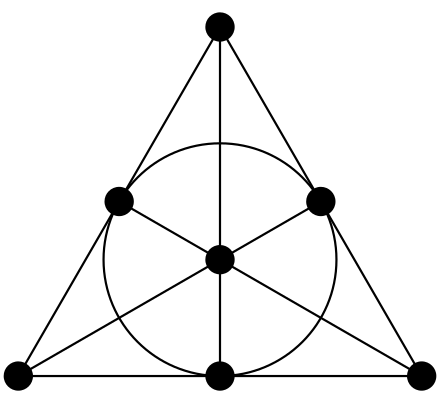
\includegraphics[scale=0.2]{20-4.png}
    \end{figure}
\end{example}

\begin{theorem}[De Bruijn-\Erdos{}~\cite{bruijn1951colour}]
    Let $P$ be a set of $n$ points in a projective plane, not all on a line, then the number of lines determined by $P$ is at least $n$.
\end{theorem}

 If the equality holds, then either $P$ is a projective plane or a graph like the following.

     \begin{figure}[H]
        \centering
        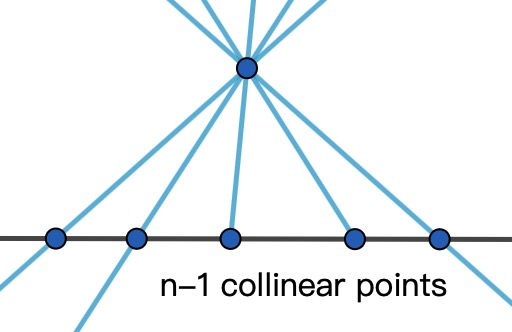
\includegraphics[scale=0.3]{20-3.jpg}
    \end{figure}

\newpage
\section{Lecture 21}

\begin{theorem}[De Bruijn-\Erdos{}~\cite{bruijn1951colour}]
    Let $P$ be a set of $n$ points in a projective plane, not all on a line, then the number of lines determined by $P$ is at least $n$.
\end{theorem}

\begin{remark}[Duality]
    The statement is also true when we swap lines and points.
\end{remark}

We prove this theorem by proving a combinatoric statement about family sets with restricted intersection.

\begin{theorem}\label{De bruijn-erdos}
    Let $\mathcal{F}\subseteq 2^{[n]}$. If for any $F,F' \in \mathcal{F}$ with $F\neq F'$, $|F\cap F'|=1$, then $|\mathcal{F}|\leq n$.
\end{theorem}

This implies the dual statement of de Bruijn-\Erdos{}. We may assume each point in $[n]$ is in at least $2$ sets in $\mathcal{F}$. Now $\mathcal{F}$ is the set of lines $L$ and ground set $[n]$ is the points determined by $\mathcal{F}=L$.

\begin{proof}[Proof of Theorem~\ref{de bruijn-erdos}]
    Consider the incidence matrix of $\mathcal{F}$, denoted as $M$. The colunms are $[n]$ and the rows are $\{ F_{1},\ldots,F_{m} \}=\mathcal{F}$. The $(i,j)$-entry is $1$ if $j\in F_{j}$, otherwise the $(i,j)$-entry is $0$. So each set in $\mathcal{F}$ corresponds to a vector in $\{ 0,1 \}^{n}$. Note that if $\{ \boldsymbol{f}_{i}\coloneqq\mathbf{1}_{F_{i}} \}_{i=1}^{m}$ are linearly independent, then $|\mathcal{F}|\leq \dim M =n$. So we can consider the form $\sum_{i=1}^{m} \alpha_{i}\boldsymbol{f}_{i}\coloneqq \boldsymbol{x}$.

    $$\langle \boldsymbol{x},\boldsymbol{x} \rangle = \Big\langle \sum_{i=1}^{m} \alpha_{i}\boldsymbol{f}_{i},\sum_{i=1}^{m} \alpha_{i}\boldsymbol{f}_{i} \Big\rangle = \sum_{i,j}\alpha_{i}\alpha_{j}\langle \boldsymbol{f}_{i},\boldsymbol{f}_{j} \rangle,$$
    where
    $$\langle \boldsymbol{f}_{i},\boldsymbol{f}_{j} \rangle = \left\{
    	\begin{aligned}
    	&|F_{i}| \quad &i=j\\
    	&1 \quad &i\neq j\\
    	\end{aligned}
    	\right
    	..
    $$
    Then
    $$\langle \boldsymbol{x},\boldsymbol{x} \rangle = \sum_{i=1}^{m}\alpha_{i}^{2}|F_{i}|+\sum_{i\neq j}\alpha_{i}\alpha_{j}=\sum_{i=1}^{m}\alpha_{i}^{2}(|F_{i}|-1)+(\sum_{i=1}^{m}\alpha_{i})^{2}.$$
    
    Assume that each $|F_{i}|\geq 2$, then $\langle \boldsymbol{x},\boldsymbol{x} \rangle=0$ if and only if $\alpha_{i}=0$ for every $i\in [m]$, which means $\{ \boldsymbol{f}_{i} \}_{i=1}^{m}$ are linearly independent.

    Without loss of generality, we can assume that $F_{1}=\{ 1 \}$. Then $|F_{1}\cap F_{i}|=1$ indicates that $1\in F_{i}$ for all $i=1,\ldots,m$. Since $|F_{i}\cap F_{j}|=1$, then $\{ F_{i}\backslash\{ 1 \} \}_{i=1}^{m}$ are pairwise disjoint, which means $|\mathcal{F}|\leq n$.
\end{proof}

\begin{remark}
    The bound of Theorem~\ref{de bruijn-erdos} is tight: we can choose $\{ 1 \},\{ 1,2 \},\{ 1,3 \},\ldots,\{ 1,n \}$ or $\{ 2,3,\ldots,n \},\{ 1,2 \},\{ 1,3 \},\ldots,\{ 1,n \}$.
\end{remark}

\subsection{Sets with at most two distinct distances}

Let $P$ be a set of points in $\mathbf{R}^{n}$ with pairwise distance one, then $|P|\leq n+1$ and we can take regular simplex to match the bound. The question in this part is: what is the maximum size of $|P|$ if we allow two distinct distances?

In $\mathbf{R}^{n}$, we can take $P=\{ e_{i}+e_{j} \}_{i,j\in \binom{[n]}{2}}$, then $|P|=\binom{n}{2}$. This is a lower bound, which is close to the best upper bound $\binom{n+2}{2}$ proved by Blokhuis~\cite{blokhuis1981new}. In this part, we will prove a slightly weaker bound.

\begin{theorem}
    Let $X\subseteq \mathbf{R}^{n}$ with at most two distinct distances between pairs of its points, then $|X|\leq \frac{1}{2}(n+4)(n+1)$.
\end{theorem}

\begin{proof}
    Let $X=\{ \boldsymbol{v}_{1},\ldots,\boldsymbol{v}_{t} \}$ and $d,D$ be the two distinct distances. Let $\boldsymbol{x}\in \mathbf{R}^{n}$, Associate to each point $\boldsymbol{v}_{i}\in X$ the following $n$-variate deg-$4$ polynomial $P_{i}$:
    $$P_{i}(\boldsymbol{x})=(\Vert \boldsymbol{x}-\boldsymbol{v}_{i} \Vert^{2}-d^{2})(\Vert \boldsymbol{x}-\boldsymbol{v}_{i} \Vert^{2}-D^{2}),$$
    where $\Vert \cdot \Vert$ is $l_{2}$-norm.

    \begin{claim}\label{pi linearly independent}
        $\{ P_{i} \}_{i\in [t]}$ are linearly independent.
    \end{claim}
    \begin{proof}[Proof of Claim~\ref{pi linearly independent}]
        Note that
        $$P_{i}(\boldsymbol{v}_{j})=\left\{
    	\begin{aligned}
    	&d^{2}D^{2} \quad &i=j\\
    	&0 \quad &i\neq j\\
    	\end{aligned}
    	\right
    	.
        $$

        If $\sum_{i\in [t]}\alpha_{i}P_{i}=0$, then for any $j\in [t]$, we have
        $$0=\sum_{i\in [t]}\alpha_{i}P_{i}(\boldsymbol{v}_{j})=\alpha_{j}d^{2}D^{2},$$
        which indicates $\alpha_{j}=0$ for all $j\in [t]$.
    \end{proof}

    Since each $P_{i}$ is polynomial with degree $4$, we get $|X|=O(n^{4})$. This bound is far from what we want, so we need to find a more economic set of vectors spanning $P_{i}$'s.

    Note that
    $$\Vert \boldsymbol{x}-\boldsymbol{v}_{i} \Vert^{2}=\sum_{j\in [n]} x_{j}^{2}-2\sum_{j\in[n]}x_{j}v_{ij}+\sum_{j\in [n]}v_{ij}^{2}.$$

    This implies $P_{i}$ is a linear combination of the following polynomials:
    
    \begin{itemize}
        \item $(\sum_{j\in [n]} x_{j}^{2})^{2}$,
        \item $x_{k}\sum_{j\in [n]}x_{j}^{2}$, for $k\in [n]$,
        \item $x_{j}x_{k}$, for $1\leq j\leq k\leq n$,
        \item $x_{j}$, for $j\in [n]$,
        \item $1$.
    \end{itemize}

    So the dimension of the space containing all $\{ P_{i} \}_{i\in [n]}$ is at most $\frac{1}{2}(n+4)(n+1)$.
\end{proof}

\subsection{Forbidding a single intersection size}

Blabla...

\begin{theorem}[Frank-Wilson~\cite{frankl1981intersection}]\label{frank wilson}
    Let $p$ be an odd prime and $\mathcal{F}\subseteq 2^{[n]}$. If
    
    \begin{itemize}
        \item for any $F\in \mathcal{F}$, $|F|\equiv 0\ (mod\ p)$,
        \item for any $F,F'\in \mathcal{F}$ with $F\neq F'$, $|F\cap F'|\not\equiv 0\ (mod\ p)$.
    \end{itemize}
    
    Then $|\mathcal{F}|\leq \binom{n}{0}+\binom{n}{1}+\cdots+\binom{n}{p-1}$.
\end{theorem}

\begin{remark}
    Blabla...
\end{remark}

\begin{proof}[Proof of Theorem~\ref{frank wilson}]
    Blabla...
\end{proof}


\newpage
\bibliographystyle{plain}
\bibliography{ref.bib}
\label{key}

\end{document}